\documentclass[12pt, a4paper]{report}

\usepackage[utf8]{inputenc}
\usepackage{graphicx} % Load actual image files
\usepackage{amsmath}  % Math environments (align, equation, etc.)
\usepackage{amssymb}  % Mathematical symbols including \mathbb (real numbers, etc.)
\usepackage{hyperref}
\usepackage[margin=1in]{geometry}
\usepackage{titlesec}
\usepackage[nottoc]{tocbibind}
\usepackage{listings}
\usepackage{xcolor}
\usepackage{float}
\usepackage{setspace}
\usepackage{longtable}
\usepackage{booktabs}
\usepackage{tabularx}
\usepackage{array}

% Standard document spacing
\usepackage{parskip} % Adds space between paragraphs automatically

% Code Listing Style
\definecolor{codegreen}{rgb}{0,0.6,0}
\definecolor{codegray}{rgb}{0.5,0.5,0.5}
\definecolor{codepurple}{rgb}{0.58,0,0.82}
\definecolor{backcolour}{rgb}{0.95,0.95,0.92}
\lstdefinestyle{mystyle}{
    backgroundcolor=\color{backcolour},   
    commentstyle=\color{codegreen},
    keywordstyle=\color{magenta},
    numberstyle=\tiny\color{codegray},
    stringstyle=\color{codepurple},
    basicstyle=\ttfamily\footnotesize,
    breakatwhitespace=false,         
    breaklines=true,                 
    captionpos=b,                    
    keepspaces=true,                 
    numbers=left,                    
    numbersep=5pt,                  
    showspaces=false,                
    showstringspaces=false,
    showtabs=false,                  
    tabsize=2
}
\lstset{style=mystyle}

% Define a "json" language for the listings package (used by the AI prompt blocks).
% The listings package has no built-in JSON language, so we register one here so
% that \begin{lstlisting}[language=json] renders correctly instead of erroring.
\lstdefinelanguage{json}{
    basicstyle=\ttfamily\footnotesize,
    string=[s]{"}{"},
    stringstyle=\color{codepurple},
    comment=[l]{//},
    commentstyle=\color{codegreen}\itshape,
    showstringspaces=false,
    breaklines=true,
    literate=
     *{0}{{{\color{codegreen}0}}}{1}
      {1}{{{\color{codegreen}1}}}{1}
      {2}{{{\color{codegreen}2}}}{1}
      {3}{{{\color{codegreen}3}}}{1}
      {4}{{{\color{codegreen}4}}}{1}
      {5}{{{\color{codegreen}5}}}{1}
      {6}{{{\color{codegreen}6}}}{1}
      {7}{{{\color{codegreen}7}}}{1}
      {8}{{{\color{codegreen}8}}}{1}
      {9}{{{\color{codegreen}9}}}{1}
}

\usepackage[font=small,labelfont=bf]{caption} % Strict technical report formatting for figures and tables
\usepackage{pdflscape} % For landscape orientation of large tables if necessary

% Reduce heading sizes to match technical report standards
\titleformat{\chapter}[display]
  {\normalfont\LARGE\bfseries}{\chaptertitlename\ \thechapter}{10pt}{\LARGE}
\titlespacing*{\chapter}{0pt}{-20pt}{20pt}
\titleformat{\section}
  {\normalfont\Large\bfseries}{\thesection}{1em}{}
\titleformat{\subsection}
  {\normalfont\large\bfseries}{\thesubsection}{1em}{}

\begin{document}

\begin{titlepage}
    \begin{center}
        
        % Header with Logos
        \begin{minipage}{0.2\textwidth}
            
\includegraphics[width=\linewidth, height=3cm, keepaspectratio]{figures/eng.png}
        \end{minipage}
        \hfill
        \begin{minipage}{0.55\textwidth}
            \centering
            \textbf{Port Said University}\\
            \textbf{Faculty of Engineering}\\
            \textbf{Department of Computer and Control Engineering}
        \end{minipage}
        \hfill
        \begin{minipage}{0.2\textwidth}
            
\includegraphics[width=\linewidth, height=3cm, keepaspectratio]{figures/psu.png}
        \end{minipage}

        \vspace{2cm}

        % Title
        {\LARGE \textbf{Kemora: An AI-Powered Travel Discovery Platform for Egypt}\par}
        \vspace{1cm}
        {\Large \textbf{Graduation Project 2026}\par}
        \vspace{1cm}
        
        % Project Logo Placeholder
        
\includegraphics[width=5cm, height=5cm, keepaspectratio]{figures/project_logo.png}
        
        \vfill

        % Details Table
        \begin{table}[H]
            \centering
            \renewcommand{\arraystretch}{1.8}
            \begin{tabular}{|>{\raggedright\arraybackslash}p{4.5cm}|>{\raggedright\arraybackslash}p{8cm}|}
                \hline
                \textbf{Supervisor} & Dr. Rabab Farouk \\
                \hline
                \textbf{Team Members} & 
                Mohamed Ahmed Mousad \newline
                Mohamed Khaled Elsayed \newline
                Zeyad Khaled Elsayed \newline
                Mohamed Eltabey Elshenawy \newline
                Ahmed Bassem Elshafey \\
                \hline
                \textbf{Department Name} & Department of Computer and Control Engineering \\
                \hline
                \textbf{Date of Submission} & July 2026 \\
                \hline
            \end{tabular}
        \end{table}

    \end{center}
\end{titlepage}

\pagenumbering{roman}
\addcontentsline{toc}{part}{1. Front Matter (Preliminary Sections)}

\chapter*{Abstract}
\addcontentsline{toc}{chapter}{Abstract}

The tourism industry in Egypt is heavily fragmented, leaving modern travelers struggling to plan logical itineraries while simultaneously discovering off-the-beaten-path ``hidden gems.'' Existing tools either offer generic AI generation with severe geographic hallucinations or simple static maps with no intelligent routing. To solve this, this project presents \textbf{Kemora}, a comprehensive TravelTech ecosystem integrating a high-performance .NET 10 Clean Architecture backend with a 60fps Flutter cross-platform mobile application. To solve AI hallucinations, Kemora implements a deterministic Retrieval-Augmented Generation (RAG) pipeline, dynamically fetching real, localized Points of Interest (POIs) from the Google Places API and a seeded local database within a 30km radius before injecting them into an OpenRouter-hosted Large Language Model (LLM). Empirical benchmarking confirms the cached read path serves requests with a median latency around 100\,ms and sustains robust, error-free throughput up to 2000 concurrent requests via aggressive \texttt{IMemoryCache} reuse, while transitioning from sequential API fetching to in-memory Zero-Fetch Image Injection eradicated database concurrency bottlenecks. Future iterations should transition to a Microservices Architecture deployed via Kubernetes, implement an offline-first mobile architecture utilizing SQLite/Hive, and natively fine-tune open-source LLMs using LoRA techniques to completely eliminate third-party dependencies.

\newpage
\input{acknowledgments}

\newpage
\tableofcontents
\newpage
\listoffigures
\addcontentsline{toc}{chapter}{List of Figures}
\newpage
\listoftables
\addcontentsline{toc}{chapter}{List of Tables}
\newpage

\pagenumbering{arabic}
\addcontentsline{toc}{part}{Body of the Report}

\chapter{Introduction}

\section{Background and Motivation}
Tourism has historically been, and remains, a vital and foundational pillar of the Egyptian economy. Egypt boasts a uniquely diverse portfolio of attractions that spans millennia, ranging from the ancient Pharaonic monuments in Luxor and Aswan, to pristine coastal resorts and diving havens in the Red Sea and Sinai, alongside a burgeoning sector of eco-tourism and medical tourism. Recent statistics underscore the sector's monumental economic impact. During the 2023 and 2024 periods, the Egyptian tourism sector experienced record-breaking growth. In the 2024/2025 fiscal year, tourism revenues reached an unprecedented \$16.7 billion, representing a massive 56.1\% growth over previous periods, driven by an influx of over 15.7 million tourists. Furthermore, the sector's direct contribution to Egypt's GDP rose to 3.7\%, with tourist nights increasing to approximately 179.3 million. 

Despite this wealth of attractions and strong economic performance, the global travel industry is undergoing a rapid digital transformation, and the expectations of the modern traveler have evolved significantly. Today's tourists demand highly personalized, instantly accessible, and community-driven digital experiences. The academic literature on artificial intelligence (AI) in tourism frequently highlights \textit{fragmentation} as a primary challenge that hinders the development of seamless, holistic, and user-centric travel experiences. 

In the Egyptian context, travelers frequently encounter a highly fragmented digital ecosystem. To plan a comprehensive multi-day trip, a user must typically navigate multiple disparate platforms: one aggregator for flight and hotel bookings, a separate directory for discovering local restaurants or cafes, a third application for mapping and geographical logistics, and yet another social network for reading reviews or connecting with other travelers. This information fragmentation leads to cognitive overload and suboptimal travel planning. Furthermore, while generic global travel platforms exist, they often lack the deep, localized context required to truly optimize an Egyptian itinerary. Such optimization requires understanding local transportation nuances, seasonal operating hours, and accurately grouping proximate attractions to minimize travel time within congested cities like Cairo or along the expansive Nile Valley.

The motivation for this graduation project stems from the urgent desire to unify these disjointed experiences into a single, cohesive, and intelligent platform. By leveraging the latest advancements in Artificial Intelligence---specifically Generative Large Language Models (LLMs) and Retrieval-Augmented Generation (RAG) paradigms---alongside modern cross-platform mobile development architectures, there is an unprecedented opportunity to automate the labor-intensive process of itinerary creation while simultaneously fostering a vibrant, localized community of travelers.

\section{The Economic and Systemic Problem Statement}
The core problem addressed by this project is the profound inefficiency and fragmentation of the modern travel planning and discovery process in Egypt. This fragmentation is not merely a user-experience hurdle; it represents a tangible economic problem. When travelers face friction in planning, they naturally default to the path of least resistance: visiting only the primary, globally recognized tourist hubs such as the Pyramids of Giza or the Luxor Temple. Consequently, thousands of ``hidden gems''---ranging from authentic local eateries in Cairo's Islamic districts to pristine, lesser-known coastal eco-lodges along the Red Sea---remain undiscovered by the average tourist. This leads to an unequal distribution of tourism revenue, overcrowded primary landmarks, and a failure to showcase the true, multifaceted cultural depth of Egypt to the world. Kemora directly addresses this by making the discovery of these hidden gems as effortless as booking a ticket to the Pyramids.

Academic research indicates that existing digital solutions often specialize in isolated functionality rather than providing an end-to-end planning ecosystem. Specifically, the problems can be categorized into four primary domains:

\begin{enumerate}
    \item \textbf{Complex and Time-Consuming Itinerary Generation:} Planning a multi-day trip requires solving what is essentially a variation of the Traveling Salesman Problem, balancing geographical proximity of activities, realistic time allocation, fatigue management, and alignment with personal budgets and interests. Doing this manually across disparate apps is tedious and prone to human error.
    
    \item \textbf{Limitations of Current AI and Propensity for Hallucination:} While Generative AI has democratized access to travel advice, generic AI chatbots (like standard ChatGPT without web-grounding) suffer from a lack of contextual awareness and severe hallucinations. In the tourism domain, this manifests as recommending non-existent places, permanently closed restaurants, or geographically impossible routes (e.g., scheduling a morning visit to the Pyramids of Giza and an afternoon lunch in Sharm El-Sheikh on the same day). The literature points to a significant data integration gap, where AI fails to utilize real-time, verified POI (Point of Interest) data.
    
    \item \textbf{Disconnect Between Discovery and Community:} Existing platforms isolate the planning phase from the social sharing phase. Travelers rely on social media (e.g., Instagram, TikTok) for inspiration, but cannot easily convert a friend's travel post or a viral video directly into an actionable, mapped item on their own itinerary. This disconnect breaks the user journey.
    
    \item \textbf{Low Engagement and Retention in Travel Apps:} Traditional utility-focused travel apps suffer from high churn rates; they are frequently deleted post-trip due to a lack of ongoing engagement mechanisms. Without a social or gamified component, there is no incentive for the user to return to the application until their next major vacation.
\end{enumerate}

\section{Competitive Analysis}
To contextualize the proposed solution, it is necessary to conduct a deep competitive analysis comparing the envisioned system against existing market incumbents. The current landscape is dominated by four archetypes of platforms, each exhibiting critical shortcomings when applied to the Egyptian market:

\subsection{Global Aggregators and Review Platforms (e.g., TripAdvisor, Expedia)}
\textbf{Strengths:} Massive global databases of reviews, standardized booking interfaces, and high brand trust. \\
\textbf{Weaknesses:} These platforms are inherently broad and lack deep, localized curation. Their itinerary generation features are typically rigid, relying on pre-packaged static tours rather than dynamically generated, personalized schedules. Furthermore, they function primarily as utility directories rather than cohesive social networks, making organic discovery feel clinical rather than inspiring.

\subsection{Generic AI Chatbots and Planners (e.g., ChatGPT, Roamr)}
\textbf{Strengths:} Highly conversational, capable of understanding complex natural language constraints, and instantaneous generation of text-based itineraries. \\
\textbf{Weaknesses:} As highlighted in recent literature, these systems suffer from systemic data hallucinations. Because they are not deeply integrated with local Egyptian geographical APIs or live business status directories, they frequently recommend logically flawed routes or closed venues. They also lack a visual, interactive map-based interface to execute the plan.

\subsection{Social Media Networks (e.g., Instagram, TikTok)}
\textbf{Strengths:} Unparalleled visual inspiration, highly engaging algorithms, and massive user bases driving organic discovery of hidden gems. \\
\textbf{Weaknesses:} They are completely devoid of practical planning tools. When a user discovers a beautiful cafe in Alexandria on TikTok, transferring that inspiration into a structured, routed daily itinerary requires switching to Google Maps and manually saving coordinates. The inspiration cannot be natively converted into an actionable trip.

\subsection{Localized Egyptian Directories (e.g., Elmenus, Cairo360)}
\textbf{Strengths:} Excellent, highly accurate, and hyper-localized data regarding specific niches (e.g., Elmenus for dining, Cairo360 for events). \\
\textbf{Weaknesses:} They are heavily siloed. A traveler cannot use Elmenus to plan a visit to the Egyptian Museum, nor can they use it to book a hotel. They solve a micro-problem rather than the macro-problem of holistic travel planning.

\section{Proposed Solution: Kemora}
To overcome the limitations of the current fragmented landscape, we propose \textbf{Kemora}, an intelligent, all-in-one travel discovery and social platform natively designed for the Egyptian context. Kemora is envisioned as the ultimate companion for navigating Egypt, bridging the gap between AI-driven planning and human-centric social discovery. The platform’s architecture provides four core pillars:

\subsection{Intelligent Trip Planning via RAG}
Kemora features a sophisticated AI-driven trip planner. By inquiring about the user's destination, budget, travel style (e.g., historical, relaxation, adventure), and duration, the system dynamically curates a day-by-day, hour-by-hour itinerary. Crucially, the system mitigates the AI hallucination problem by implementing a robust Retrieval-Augmented Generation (RAG)-like pipeline. Rather than relying on the LLM's parametric memory, the backend pre-fetches verified, highly-rated places from external APIs (such as Foursquare) within a strict geographical radius. This constrained, localized dataset is then injected into the LLM's context window. This strict architectural decision ensures the AI only recommends real, currently open, and geographically proximate locations, entirely eliminating impossible routing.

\subsection{Social Discovery and Community Integration}
Unlike utility-only apps, Kemora integrates a fully-fledged social network. Users can share posts, upload media, react, comment, and follow other travelers. This transforms the application from a transient planning tool into a source of continuous, daily inspiration. Most importantly, users can explore feeds of content generated by others and seamlessly ``bookmark'' or extract places mentioned in posts, directly injecting them into their personal itineraries. This solves the disconnect between inspiration and execution.

\subsection{Interactive Exploration and Editorial Context}
The application provides an interactive map and a rich directory of Egyptian governorates. Users can explore specific cities, read detailed editorial descriptions, view high-quality image galleries, and filter attractions by granular categories (Hotels, Restaurants, Cafes, Landmarks, Medical Tourism hubs). This ensures that even users who prefer manual planning over AI generation have access to a centralized, beautiful discovery interface.

\subsection{Gamification and Retention Mechanisms}
To drive continuous user engagement and combat post-trip app deletion, Kemora employs a deep gamification system. Users earn points, level up, and unlock badges for contributing to the community (e.g., publishing high-quality posts, leaving detailed reviews, completing planned trips). This system incentivizes a rich, user-generated content ecosystem that continually improves the platform's proprietary data quality and creates a sticky, retaining user experience.

\section{Project Objectives}
The primary objectives of this graduation project are to deliver a production-ready software ecosystem. Specifically:
\begin{itemize}
    \item \textbf{Full-Stack Engineering:} To design, develop, and deploy a robust, highly responsive full-stack application utilizing a modern Flutter frontend for cross-platform mobile delivery, backed by a high-performance .NET 10 Web API.
    \item \textbf{Clean Architecture Implementation:} To rigorously apply Clean Architecture principles and Domain-Driven Design (DDD) on the backend. This ensures the system remains maintainable, inherently testable, and loosely coupled, allowing for future expansion.
    \item \textbf{AI Orchestration and Prompt Engineering:} To engineer a reliable AI pipeline that interacts with state-of-the-art models via OpenRouter. This involves dynamic model selection, context window management, precise prompt engineering, and strict JSON schema enforcement to ensure parsable itinerary generation.
    \item \textbf{High Performance and Scalability:} To implement effective optimization strategies, including aggressive caching (\texttt{IMemoryCache}, distributed caching) and concurrent asynchronous data fetching, ensuring low-latency API responses even during complex AI generation tasks.
    \item \textbf{Quality Assurance and Benchmarking:} To rigorously validate the system's reliability through comprehensive End-to-End (E2E) integration testing and load benchmarking, proving the backend can withstand concurrent user traffic.
\end{itemize}

\section{Document Organization}
The remainder of this thesis is structured as follows:
\begin{itemize}
    \item \textbf{Chapter 2 (Literature Review \& Technologies):} Explores the theoretical foundations of the selected technology stack, including the evolution of Flutter, the performance characteristics of .NET, the principles of Clean Architecture, and the applied theory behind Large Language Models and RAG systems.
    \item \textbf{Chapter 3 (System Analysis \& Design):} Details the system's non-functional and functional requirements, comprehensive UML diagrams (Use Case, Sequence, Activity), high-level system architecture, and complex database entity-relationship (ER) models.
    \item \textbf{Chapter 4 (Implementation):} Chronologically outlines the development phases, highlighting the evolution of the AI pipeline, UI/UX implementation challenges, and complex backend integrations such as authentication and external API routing.
    \item \textbf{Chapter 5 (Testing \& Benchmarking):} Discusses the E2E testing methodology, unit testing coverage, and presents empirical results from backend load testing and performance profiling.
    \item \textbf{Chapter 6 (Conclusion \& Future Work):} Summarizes the project's achievements, reflects on lessons learned, and outlines potential avenues for future commercial enhancement and feature expansion.
    \item \textbf{Appendix A:} Provides a comprehensive API documentation reference (Swagger/OpenAPI specifications) for the backend services.
\end{itemize}

\chapter{Literature Review \& Technology Stack}

\section{Introduction}
Building a modern, highly scalable, and artificial intelligence-integrated travel platform necessitates a meticulous and rigorous selection of underlying technologies. The architectural paradigm must seamlessly support real-time social interactions, highly complex relational data models, asynchronous integrations with external application programming interfaces (APIs), and deterministic, cross-platform mobile rendering at high frame rates. This chapter provides a comprehensive review of the theoretical background, mathematical foundations, and software engineering paradigms of the chosen technologies, establishing a scholarly justification for their selection over contemporaneous alternatives.

\section{Mobile Frontend Development: Flutter and Impeller}
\subsection{Overview of the Flutter Framework}
Flutter is an open-source, declarative UI software development kit (SDK) engineered by Google. Since its inception, it has rapidly ascended as the dominant framework for cross-platform mobile application development. Unlike traditional cross-platform frameworks such as Apache Cordova or Ionic, which rely on a WebView and HTML/CSS-based rendering, or frameworks like React Native, which utilize a JavaScript bridge to asynchronously invoke OEM (Original Equipment Manufacturer) widgets, Flutter adopts a radically divergent architectural approach. It ships with its own high-performance rendering engine, fundamentally bypassing OEM widgets to draw graphics primitives directly to the canvas provided by the host operating system.

\subsection{The Impeller Rendering Engine}
Historically, Flutter utilized the Skia 2D graphics library. However, Skia's reliance on Just-In-Time (JIT) shader compilation often led to "shader compilation jank"—dropped frames during the initial rendering of complex animations as the engine compiled shaders on the fly. 

To resolve this bottleneck, Flutter transitioned to \textbf{Impeller}, a modern rendering engine built from the ground up for Flutter's specific needs. Impeller fundamentally alters the rendering pipeline through an \textbf{Ahead-of-Time (AOT)} approach.
\begin{itemize}
    \item \textbf{AOT Shader Compilation:} Impeller pre-compiles a specialized, deterministic set of shaders at engine-build time. All pipeline state objects (PSOs) are generated upfront, mathematically guaranteeing that shader compilation will not occur during the rendering of an animation frame.
    \item \textbf{Modern Graphics APIs:} Impeller interfaces directly with low-level, modern graphics APIs—specifically \textbf{Metal} on iOS and \textbf{Vulkan} on Android (API 29+). This bypasses the overhead of legacy abstraction layers like OpenGL.
    \item \textbf{Tessellation-based Rendering:} For complex vector paths, Impeller utilizes tessellation algorithms to break curves into primitive triangles, heavily parallelizing the rasterization process across the GPU's multi-core architecture.
\end{itemize}
This architectural shift provides predictable, 120-frames-per-second (fps) performance, crucial for maintaining user immersion in a visually rich travel application like Kemora.

\subsection{The Dart Programming Language}
Flutter's underlying logic is executed via Dart, a client-optimized, strictly-typed, object-oriented language. Dart provides a dual-compilation paradigm that accelerates both the development lifecycle and runtime execution:
\begin{enumerate}
    \item \textbf{Just-In-Time (JIT) Compilation:} During the development phase, the Dart Virtual Machine executes code via JIT compilation. This enables "Stateful Hot Reload," allowing developers to inject updated source code into the running virtual machine without losing the application state.
    \item \textbf{Ahead-Of-Time (AOT) Compilation:} For production artifacts, Dart compiles directly to native ARM machine code. This eliminates the overhead of a virtual machine interpretation at runtime, ensuring deterministic memory allocation and fast startup times.
\end{enumerate}

\subsection{Declarative UI and State Management Architecture}
Flutter employs a declarative UI paradigm, an evolution from imperative UI models where the developer manually mutates the UI state. In Flutter, the UI is a pure function of the state: $UI = f(state)$. Everything from padding models to interactive buttons is an immutable \texttt{Widget}. When the state changes, the framework reconstructs the widget tree and computes a diff against the element tree, selectively updating the underlying render objects.

For state management, Kemora integrates the \texttt{Provider} package, an optimized wrapper around Flutter's inherently $O(1)$ \texttt{InheritedWidget} propagation mechanism. This completely eliminates "prop-drilling" in deep widget trees. To maintain separation of concerns, the frontend architecture rigorously adheres to the principles of Clean Architecture, isolating Presentation logic (View and ViewModels) from Domain operations (Entities and UseCases).

\section{Backend Architecture: .NET 10 and C\#}
\subsection{Runtime Enhancements in .NET 10}
The backend application programming interface (API) is powered by Microsoft's .NET 10, the most advanced iteration of the cross-platform .NET ecosystem. .NET 10 introduces critical enhancements at the runtime level. The Tiered Compilation system has been heavily optimized, incorporating aggressive loop unrolling, enhanced escape analysis, and refined Dynamic PGO (Profile-Guided Optimization). These JIT improvements allow the runtime to minimize heap allocations by promoting short-lived objects to the stack, significantly reducing the pressure on the Garbage Collector (GC) and enabling massive throughput under high concurrency.

\subsection{Kestrel Web Server and TechEmpower Benchmarks}
ASP.NET Core utilizes Kestrel, an asynchronous, event-driven web server. Kestrel's architecture relies heavily on non-blocking I/O multiplexing (e.g., \texttt{epoll} on Linux) and advanced memory pooling techniques via \texttt{Span<T>} and \texttt{Memory<T>}, enabling zero-copy parsing of HTTP requests. 

Consequently, Kestrel consistently ranks in the top tier of the rigorous \textbf{TechEmpower Framework Benchmarks}. Specifically, in Plaintext and JSON serialization workloads, Kestrel demonstrates industry-leading throughput, capable of processing millions of requests per second on standard hardware. This raw performance is indispensable for Kemora, as the system orchestrates multiplexed asynchronous requests to external AI providers and geocoding services simultaneously.

\section{Software Engineering Paradigms: Clean Architecture}
\subsection{The Dependency Rule and Inversion of Control}
Clean Architecture, formalized by Robert C. Martin, dictates a ringed topological structure of software dependencies. The foundational axiom is the \textbf{Dependency Rule}: source code dependencies must exclusively point inward toward higher-level domain policies.

To achieve this without violating runtime execution requirements, the architecture leverages the \textbf{Dependency Inversion Principle (DIP)}, a cornerstone of SOLID design. Rather than the inner layers depending on external infrastructure (e.g., a database), the inner layer defines an abstraction (an \texttt{interface}), and the outer layer provides the concrete implementation. A robust \textbf{Dependency Injection (DI)} container resolves these interfaces at runtime.

\subsection{Service Layer Architecture and the Repository Pattern}
To manage the complexity of Kemora's data access and business rules, the application employs a \textbf{Service Layer} architecture. Rather than segregating reads and writes via a CQRS pattern, the conceptual model aggregates related domain behaviors into highly cohesive, modular service classes (e.g., \texttt{TripPlannerService}, \texttt{PlaceManagementService}). This design minimizes architectural boilerplate, encapsulates transaction boundaries, and coordinates workflows seamlessly between the web presentation layer and the domain logic.

Complementing the Service Layer is the \textbf{Repository Pattern}. The Repository acts as an in-memory collection abstraction over the persistent data store. By utilizing interface-driven repositories (e.g., \texttt{ITripRepository}), the domain logic remains entirely agnostic of the underlying ORM (Entity Framework Core) or relational database dialect.

\section{The Mathematics of Large Language Models (LLMs)}
\subsection{Transformer Architecture and Token Processing}
The generative AI capabilities within Kemora are powered by transformer-based Large Language Models (LLMs). Unlike legacy Recurrent Neural Networks (RNNs) that process sequences sequentially, the Transformer architecture introduced by Vaswani et al. (2017) processes tokens in parallel via the mechanism of Self-Attention.

The text processing pipeline involves several mathematical transformations:
\begin{enumerate}
    \item \textbf{Tokenization and Embedding:} The input string is tokenized into a sequence of indices, $X = [x_1, x_2, \dots, x_n]$. Each token is mapped to a high-dimensional vector space, resulting in an embedding matrix $E \in \mathbb{R}^{n \times d_{model}}$.
    \item \textbf{Positional Encoding:} Since parallel processing loses sequential order, a positional encoding matrix $P$, often utilizing deterministic sine and cosine functions of varying frequencies, is added to the embeddings: $E_{pos} = E + P$.
\end{enumerate}

\subsection{The Self-Attention Mechanism}
The core innovation of the Transformer is the Scaled Dot-Product Attention mechanism. For a given input matrix, three distinct linear transformations (learned weight matrices $W_Q, W_K, W_V$) are applied to project the input into Queries ($Q$), Keys ($K$), and Values ($V$):
$$ Q = X W_Q, \quad K = X W_K, \quad V = X W_V $$
The attention scores are then computed mathematically. The dot product of the Queries and Keys establishes the semantic relevance between all pairs of tokens. To prevent gradient vanishing during backpropagation caused by massive dot products, the result is scaled by the square root of the key dimension, $\sqrt{d_k}$. Finally, a softmax function normalizes the scores into a probability distribution, which is multiplied by the Values:
$$ \text{Attention}(Q, K, V) = \text{softmax}\left(\frac{QK^T}{\sqrt{d_k}}\right)V $$
This allows the LLM to selectively focus ("attend") on different parts of the context window when predicting the next token, enabling the synthesis of highly coherent, contextually aware JSON itineraries.

\subsection{Mitigating Hallucinations via RAG}
A critical vulnerability of stochastic autoregressive LLMs is "hallucination"—the generation of mathematically probable but factually incorrect assertions. To guarantee the reliability of Kemora's travel itineraries, the system implements \textbf{Retrieval-Augmented Generation (RAG)}.

Instead of relying on the LLM's parametric memory (weights learned during pre-training), RAG introduces an external, deterministic retrieval phase. Before model inference, Kemora's backend queries the Google Places API and a curated geographic database (highly optimized for locations in Egypt) to retrieve an exact, verified subset of active locations. This geospatial data is syntactically injected into the LLM's system prompt context window. The LLM is strictly constrained via instruction tuning to orchestrate only the retrieved entities, effectively converting the generative model from an unreliable "oracle of facts" into a robust natural language routing algorithm with algorithmically grounded precision.

\subsection{OpenRouter Integration}
To avoid vendor lock-in and ensure high availability, Kemora interfaces with \textbf{OpenRouter}, a unified API gateway. This enables dynamic model routing, allowing the application to seamlessly fallback between state-of-the-art models (e.g., Llama 3, Claude 3, GPT-4o) based on latency, rate-limiting, and cost metrics, ensuring a resilient AI architecture.

\chapter{System Analysis \& Design}

\section{Introduction}
This chapter delineates the formal requirements engineering and architectural design of the Kemora platform. A robust system design is the foundation of any scalable application, ensuring that the software not only meets its current functional objectives but is also resilient to future expansion and varying loads. The architecture utilizes ASP.NET Core for the backend API and Flutter for the cross-platform mobile frontend.

\section{Requirements Specification}

\subsection{Functional Requirements}
Functional requirements define the specific behaviors and functions the system must perform. The core functional requirements for Kemora are:
\begin{itemize}
    \item \textbf{FR1 - User Authentication \& Authorization:} The system must allow users to register, log in (via email/password or Google OAuth), and securely manage their sessions. Authentication is handled via JWT tokens, with support for token refresh, email confirmation, and password reset functionalities.
    \item \textbf{FR2 - Destination Discovery:} The system must display a categorized directory of Egyptian governorates and specific tourist attractions, augmented with images (via Cloudinary) and metadata (via Google Places).
    \item \textbf{FR3 - AI Trip Generation:} The system must accept user parameters (duration, budget, preferences) and generate a logically ordered, day-by-day itinerary using an external LLM (via OpenRouter).
    \item \textbf{FR4 - Trip Modification (Custom Roadmap):} Users must be able to view their generated trips on an interactive map, manually add places, remove places, and reorder itinerary items dynamically.
    \item \textbf{FR5 - Social Networking \& Community:} The system must provide a community feed where users can publish posts, attach media, leave comments, and react to content. Posts can be directly linked to user-generated AI trips.
    \item \textbf{FR6 - Gamification Engine:} The system must track user actions and automatically award points and badges (e.g., "AiPioneer", "CityHopper") upon crossing specific thresholds.
\end{itemize}

\subsection{Non-Functional Requirements}
Non-functional requirements specify criteria that judge the operation of the system, guaranteeing stability, security, and high performance.
\begin{itemize}
    \item \textbf{NFR1 - Performance \& Caching:} The backend API must respond to standard data retrieval requests in under 100ms under normal load. AI generation requests should resolve within 15 seconds. To achieve this, the system uses in-memory caching (\texttt{MemoryCacheService}) for frequent queries and caches available LLM models concurrently.
    \item \textbf{NFR2 - Scalability:} The architecture must support stateless scaling. Session state must not be stored in server memory. JWTs ensure that requests can be routed to any backend node behind a load balancer. Thread-safe operations (using \texttt{SemaphoreSlim}) ensure safe initialization of singletons like the OpenRouter model cache under high load.
    \item \textbf{NFR3 - Security Protocols:}
    \begin{itemize}
        \item \textbf{Data Encryption:} All communication is encrypted via TLS 1.2/1.3.
        \item \textbf{Password Hashing:} Passwords are cryptographically hashed using PBKDF2 (the ASP.NET Core Identity default) with a high iteration count.
        \item \textbf{JWT Structure:} JSON Web Tokens are signed using the HMAC-SHA512 algorithm (\texttt{SecurityAlgorithms.HmacSha512Signature}). Tokens contain specific claims (\texttt{NameId}, \texttt{Email}, \texttt{GivenName}, \texttt{Role}) and possess a 7-day expiration time to balance user convenience with security. Refresh tokens are generated as 32-byte cryptographically secure random numbers encoded in Base64.
        \item \textbf{Rate Limiting:} Critical endpoints (e.g., \texttt{AuthController}) are protected against brute-force and DDoS attacks via ASP.NET Core Rate Limiting (\texttt{[EnableRateLimiting("auth")]}).
    \end{itemize}
    \item \textbf{NFR4 - Maintainability:} The backend strictly adheres to Clean Architecture. The Domain layer is completely independent of external frameworks. Application logic is separated into Services (\texttt{TripService}, \texttt{TripPlannerService}), while external integrations reside in the Infrastructure layer (\texttt{AuthService}, \texttt{OpenRouterAiService}). HTTP routing is confined to the API tier (\texttt{TripsController}, \texttt{AuthController}, \texttt{PlacesController}).
\end{itemize}

\section{System Architecture}
Kemora utilizes a multi-tier, decoupled architecture designed for high cohesion and loose coupling. The backend is structured into four main layers: API, Application, Domain, and Infrastructure.

\subsection{Architectural Layers}
\begin{enumerate}
    \item \textbf{Domain Layer:} Contains core business entities (\texttt{ApplicationUser}, \texttt{Trip}, \texttt{Place}) and repository interfaces.
    \item \textbf{Application Layer:} Houses Data Transfer Objects (DTOs), business service interfaces (\texttt{ITripService}, \texttt{IAiService}), and core business logic (\texttt{TripService}, \texttt{TripPlannerService}).
    \item \textbf{Infrastructure Layer:} Implements the interfaces. Key implementations include \texttt{TokenService} for JWT handling, \texttt{OpenRouterAiService} for communicating with LLMs, and \texttt{CloudinaryImageService} for media storage.
    \item \textbf{API Layer:} Exposes RESTful endpoints (e.g., \texttt{AuthController}, \texttt{TripsController}) secured via Bearer authentication.
\end{enumerate}

\begin{figure}[H]
    \centering
    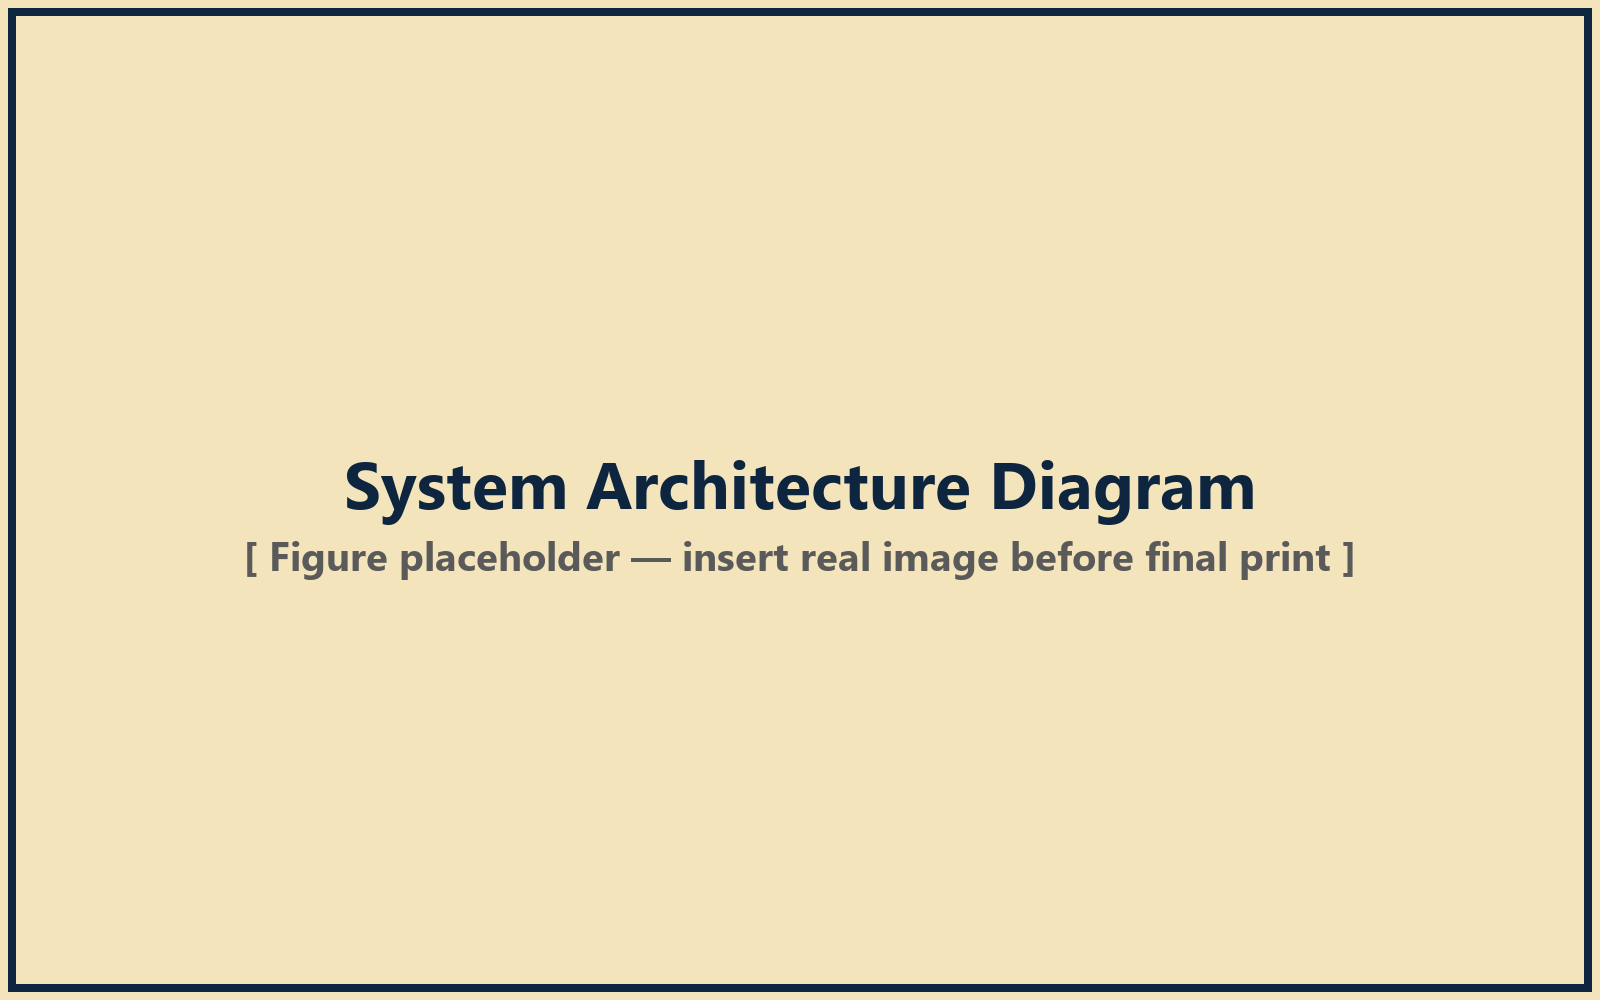
\includegraphics[width=0.9\textwidth]{figures/architecture.png}
    \caption{Kemora's Overall Architecture}
    \label{fig:architecture}
\end{figure}

\subsection{Sequence Diagrams}

\subsubsection{Authentication Flow (JWT Generation)}
The following Mermaid sequence diagram illustrates the login and token generation process when a user authenticates via the \texttt{AuthController}.

\begin{verbatim}
sequenceDiagram
    participant Client as Flutter App
    participant API as AuthController
    participant AuthSvc as AuthService
    participant SignIn as SignInManager
    participant Identity as UserManager
    participant TokenSvc as TokenService
    participant DB as SQL Server

    Client->>API: POST /api/v1/auth/login (email, password)
    API->>AuthSvc: LoginAsync(model)
    AuthSvc->>Identity: FindByEmailAsync(email)
    Identity->>DB: Query User
    DB-->>Identity: Return ApplicationUser
    AuthSvc->>SignIn: CheckPasswordSignInAsync(user, password, false)
    SignIn-->>AuthSvc: Password Valid
    AuthSvc->>TokenSvc: GenerateRefreshToken()
    TokenSvc-->>AuthSvc: Return 32-byte Base64 String
    AuthSvc->>Identity: UpdateAsync(user)
    Identity->>DB: Save Refresh Token to User
    AuthSvc->>TokenSvc: CreateTokenAsync(user)
    TokenSvc->>Identity: GetRolesAsync(user)
    Identity-->>TokenSvc: List of Roles
    Note over TokenSvc: Sign JWT with HMAC-SHA512<br/>Attach Claims (NameId, Email, GivenName, Role)
    TokenSvc-->>AuthSvc: Return JWT String
    AuthSvc-->>API: Return AuthResponseDto
    API-->>Client: 200 OK (Tokens + User Info)
\end{verbatim}

\subsubsection{AI Trip Generation \& Save Flow}
This diagram outlines the process of requesting an AI-generated itinerary and subsequently saving it to the database using the \texttt{PlacesController}, \texttt{TripsController}, and \texttt{OpenRouterAiService}.

\begin{verbatim}
sequenceDiagram
    participant Client as Flutter App
    participant PlacesAPI as PlacesController
    participant TripsAPI as TripsController
    participant PlannerSvc as TripPlannerService
    participant TripSvc as TripService
    participant AI as OpenRouterAiService
    participant ExtAI as OpenRouter API
    participant Badge as BadgeAwardService
    participant DB as SQL Server

    Client->>PlacesAPI: POST /api/v1/places/trip-plan (TripPlanRequestDto)
    PlacesAPI->>PlannerSvc: GenerateTripPlanAsync(request)
    PlannerSvc->>AI: GenerateCompletionAsync(sysPrompt, userPrompt)
    Note over AI: Check ConcurrentDictionary<br/>for available free models
    AI->>ExtAI: HTTP POST /v1/chat/completions
    ExtAI-->>AI: LLM JSON Response (Itinerary)
    AI-->>PlannerSvc: Parsed TripPlanResponseDto
    PlannerSvc-->>PlacesAPI: Return TripPlanResponseDto
    PlacesAPI-->>Client: 200 OK (Proposed Itinerary)
    
    Note over Client: User reviews and modifies<br/>the itinerary locally
    
    Client->>TripsAPI: POST /api/v1/trips/save-plan (SaveAIPlanDto)
    TripsAPI->>TripSvc: SaveAIPlanAsync(userId, dto)
    TripSvc->>DB: Insert Trip & TripPlaces
    DB-->>TripSvc: Assigned TripID
    TripSvc-->>TripsAPI: Return TripDetailDto
    
    TripsAPI->>Badge: TryAwardAiPioneerAsync(userId)
    Badge->>DB: Check/Update User Badges
    TripsAPI->>Badge: TryAwardCityHopperAsync(userId)
    TripsAPI-->>Client: 201 Created (Trip details)
\end{verbatim}

\section{Database Design and Entity Relationships}
The data tier is powered by a relational SQL Server database schema optimized for entity integrity and rapid querying. The schema is managed via Entity Framework Core Code-First migrations.

\subsection{Key Data Entities}
\begin{itemize}
    \item \textbf{ApplicationUser:} Inherits from ASP.NET Identity User. Holds authentication details, accumulated points, and JSON-serialized user preferences.
    \item \textbf{Place \& Governorate:} Hierarchical spatial data. Places are linked to Governorates via foreign keys and are categorized by \texttt{PlaceType}.
    \item \textbf{Trip \& TripPlace:} Represents the AI-generated itineraries. A \texttt{Trip} has a one-to-many relationship with \texttt{TripPlace}, representing the chronological ordering of activities (with precise \texttt{Order} fields for timeline mapping).
    \item \textbf{Post \& Comment:} The core of the social network. Posts link to a \texttt{UserID} and optionally a \texttt{LinkedTripId}, allowing users to seamlessly share their itineraries directly to the feed.
\end{itemize}

\begin{figure}[H]
    \centering
    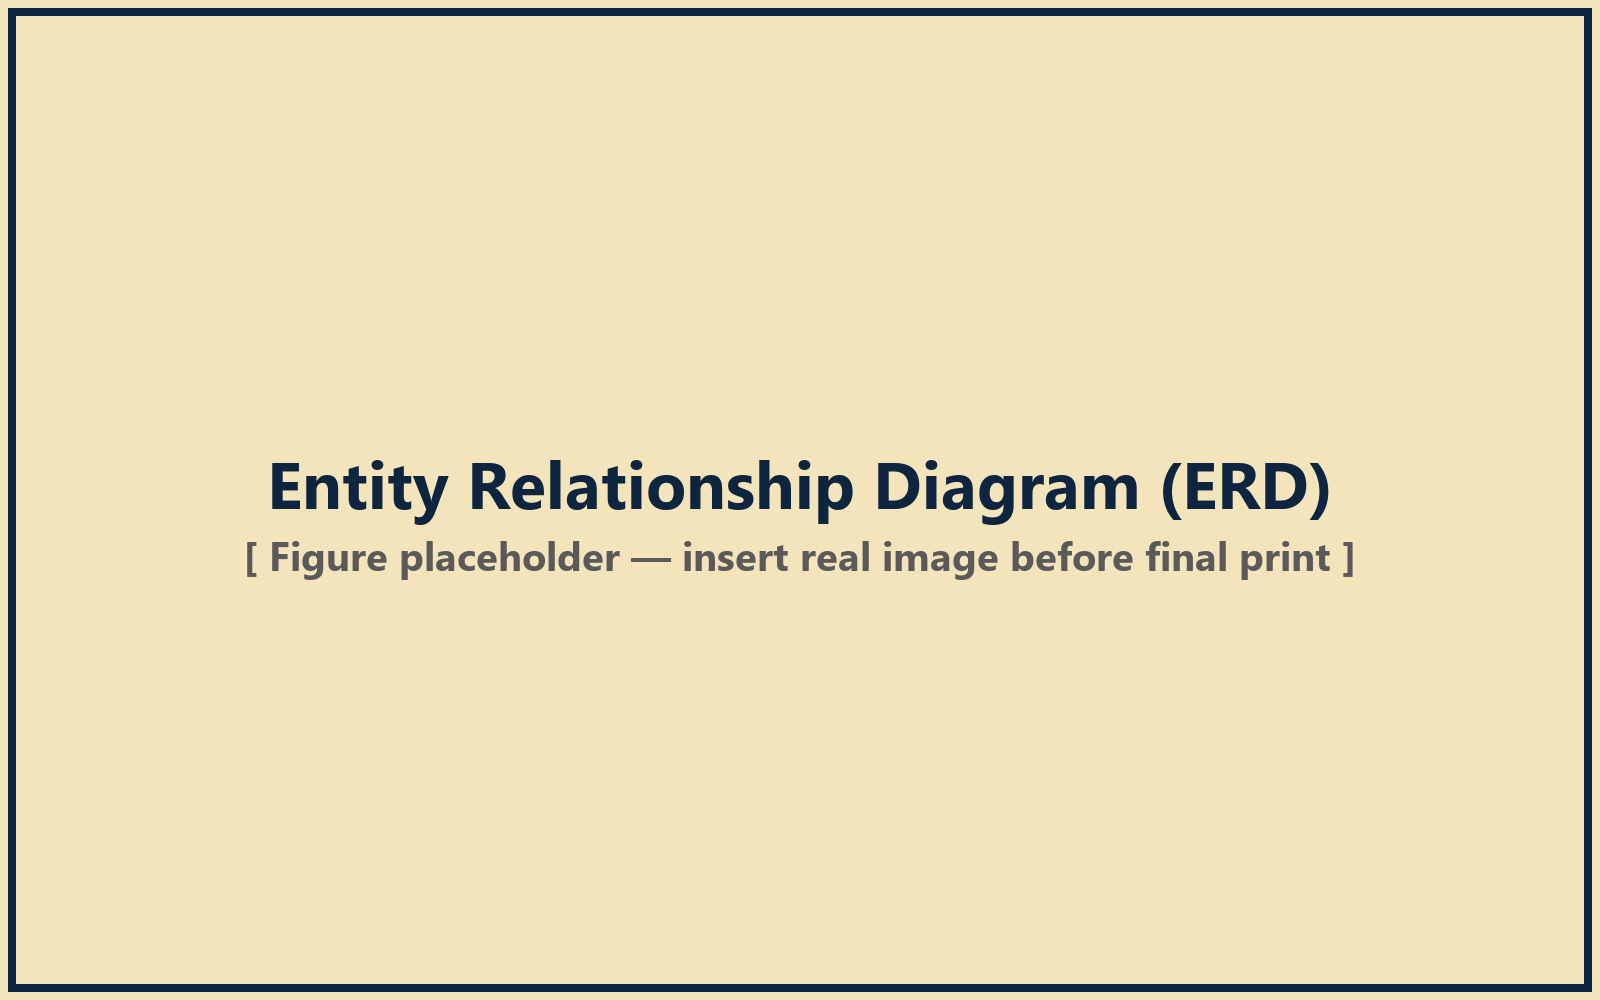
\includegraphics[width=0.9\textwidth]{figures/erd.png}
    \caption{Entity Relationship Diagram (ERD)}
    \label{fig:erd}
\end{figure}

\section{Frontend User Journeys and UI Design}
The Flutter application (`lib/presentation/`) is structurally divided by core domains. The User Interface (UI) follows a "Modern Heritage" design language—blending contemporary mobile UX patterns (glassmorphism, vibrant gradients) with culturally resonant typography and color palettes.

\subsection{Journey 1: Onboarding \& Authentication}
The user is first greeted by an animated Splash Screen, followed by an educational Walkthrough. The Authentication flow supports standard registration and OAuth. It intercepts deep links for email confirmation and password resets.

\begin{figure}[H]
    \centering
    \begin{minipage}{0.45\textwidth}
        \centering
        
\includegraphics[width=\linewidth]{figures/splash.png}
        \caption{Mobile Application Splash Screen}
        \label{fig:splash}
    \end{minipage}\hfill
    \begin{minipage}{0.45\textwidth}
        \centering
        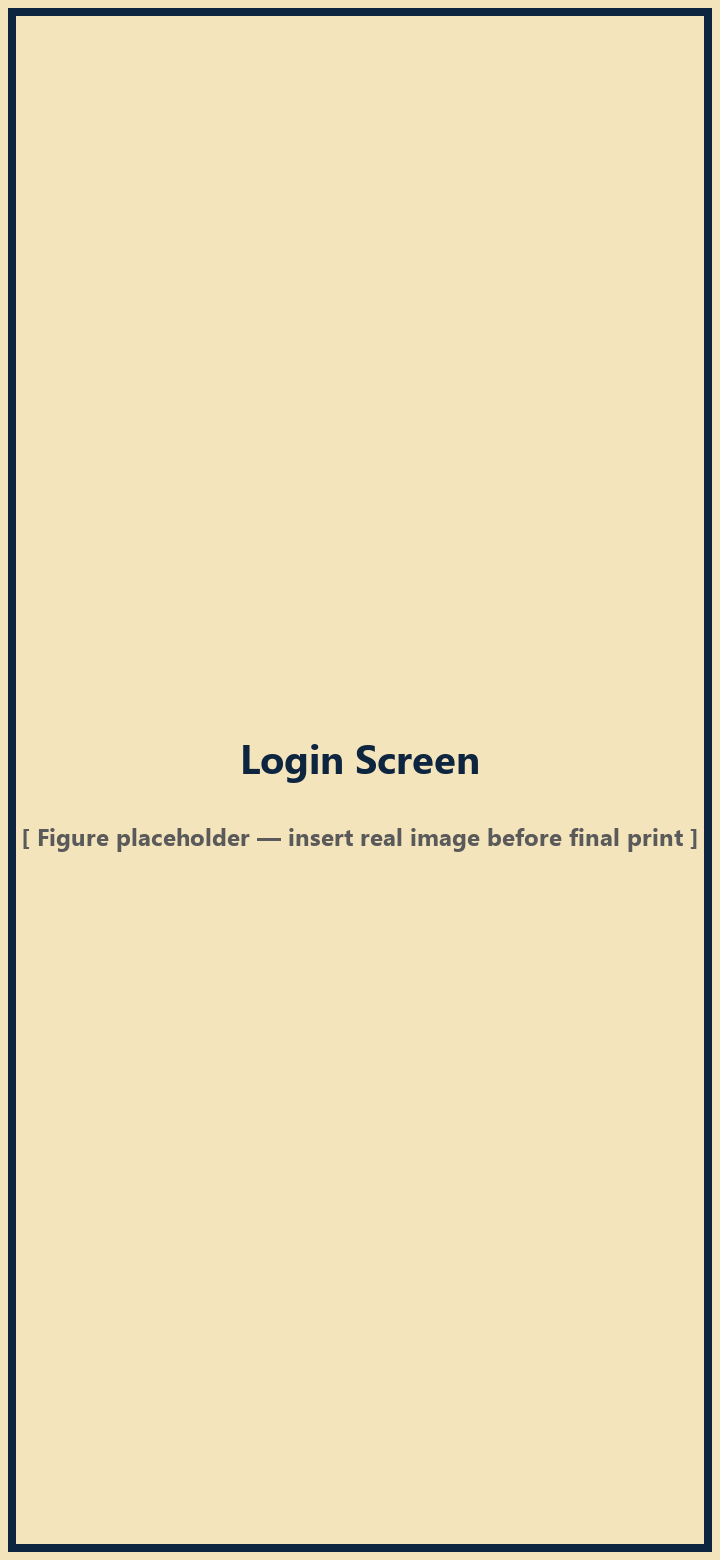
\includegraphics[width=\linewidth]{figures/login.png}
        \caption{Mobile Application Authentication Page}
        \label{fig:login}
    \end{minipage}
\end{figure}

\subsection{Journey 2: Main Dashboard \& Discovery}
The Home screen serves as the central hub, presenting personalized recommendations, top-rated destinations, and quick-action navigation via a custom floating tab bar.

\begin{figure}[H]
    \centering
    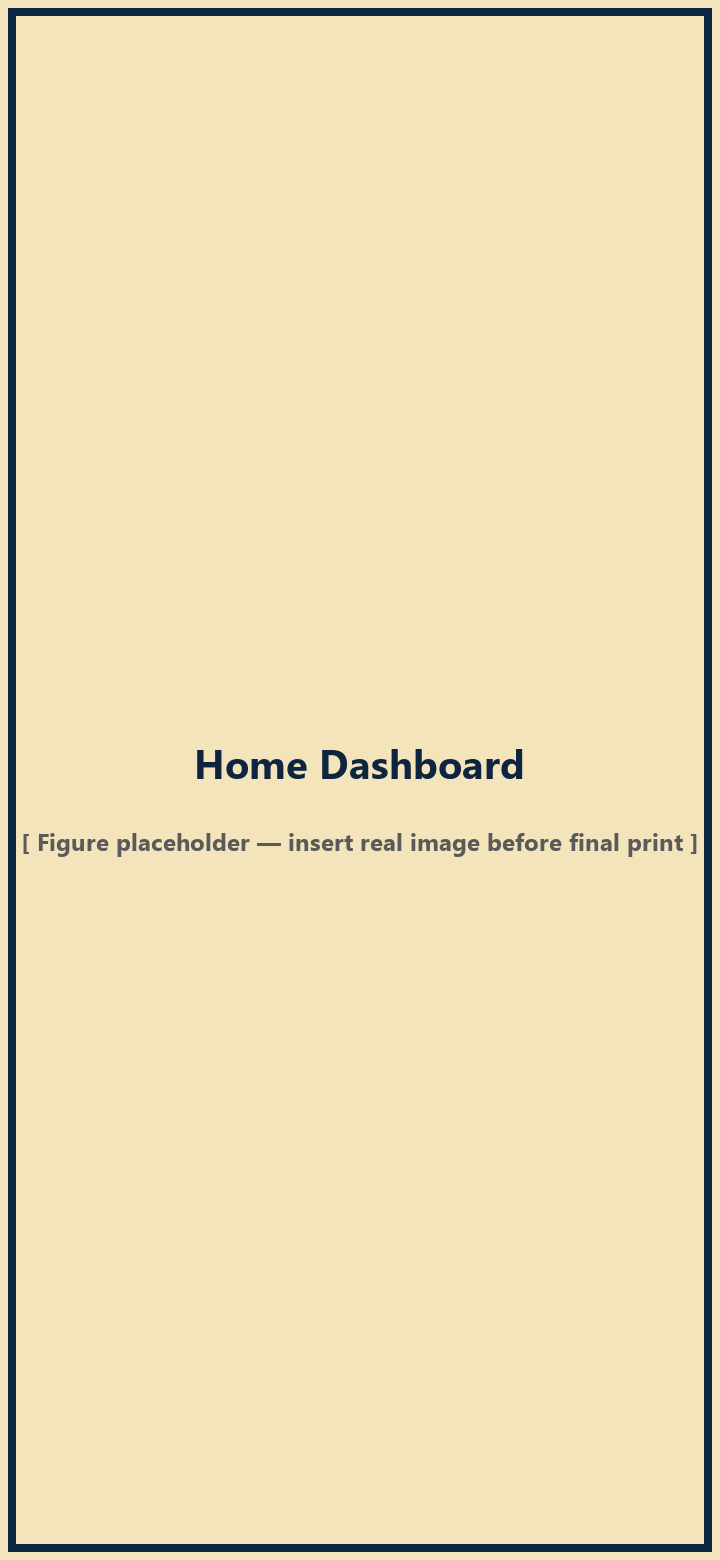
\includegraphics[width=0.45\textwidth]{figures/home.png}
    \caption{Mobile Application Home Page}
    \label{fig:home}
\end{figure}

\subsection{Journey 3: Explore \& Location Discovery}
Users can navigate an interactive map of Egyptian governorates. Selecting a governorate transitions to a detailed view listing sub-categories (Historical, Coastal, etc.) and individual Place detail screens.

\begin{figure}[H]
    \centering
    \begin{minipage}{0.3\textwidth}
        \centering
        
\includegraphics[width=\linewidth]{figures/map.png}
        \caption{Interactive Map}
        \label{fig:map}
    \end{minipage}\hfill
    \begin{minipage}{0.3\textwidth}
        \centering
        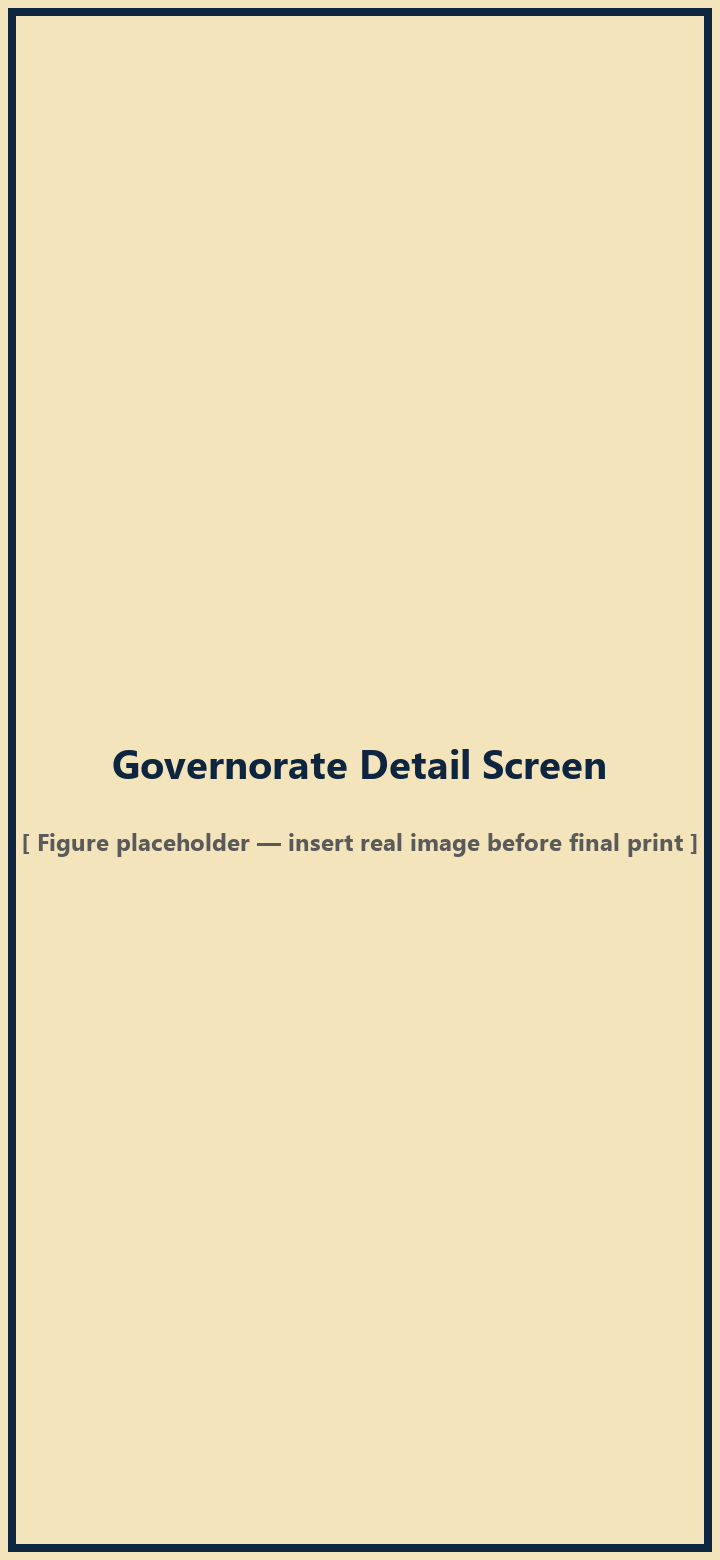
\includegraphics[width=\linewidth]{figures/gov_details.png}
        \caption{Governorate Details}
        \label{fig:gov_details}
    \end{minipage}\hfill
    \begin{minipage}{0.3\textwidth}
        \centering
        
\includegraphics[width=\linewidth]{figures/place_details.png}
        \caption{Place Details}
        \label{fig:place_details}
    \end{minipage}
\end{figure}

\subsection{Journey 4: Trip Planning \& AI Itinerary}
This is the flagship journey. Users input parameters into a multi-step questionnaire (`ai_step_questions_screen.dart`). The system displays a loading animation while negotiating with the backend AI. The result is a beautifully rendered, interactive timeline (`ai_itinerary_result_screen.dart`).

\begin{figure}[H]
    \centering
    \begin{minipage}{0.45\textwidth}
        \centering
        
\includegraphics[width=\linewidth]{figures/ai_questions.png}
        \caption{AI Trip Planner Questionnaire}
        \label{fig:ai_questions}
    \end{minipage}\hfill
    \begin{minipage}{0.45\textwidth}
        \centering
        
\includegraphics[width=\linewidth]{figures/ai_itinerary.png}
        \caption{AI Generated Itinerary Timeline}
        \label{fig:ai_itinerary}
    \end{minipage}
\end{figure}

\subsection{Journey 5: Social \& Community}
A familiar, vertically scrolling feed allows users to consume and produce content. Users can view detailed posts, engage in comment threads, and participate in direct real-time chats.

\begin{figure}[H]
    \centering
    \begin{minipage}{0.45\textwidth}
        \centering
        
\includegraphics[width=\linewidth]{figures/social_feed.png}
        \caption{Community Social Feed}
        \label{fig:social_feed}
    \end{minipage}\hfill
    \begin{minipage}{0.45\textwidth}
        \centering
        
\includegraphics[width=\linewidth]{figures/chat.png}
        \caption{Real-Time Messaging Interface}
        \label{fig:chat}
    \end{minipage}
\end{figure}

\subsection{Journey 6: Profile \& Gamification}
The Profile screen tracks the user's identity, displaying earned badges, total points, redeemed vouchers, and saved places.

\begin{figure}[H]
    \centering
    \begin{minipage}{0.45\textwidth}
        \centering
        
\includegraphics[width=\linewidth]{figures/profile.png}
        \caption{User Profile Screen}
        \label{fig:profile}
    \end{minipage}\hfill
    \begin{minipage}{0.45\textwidth}
        \centering
        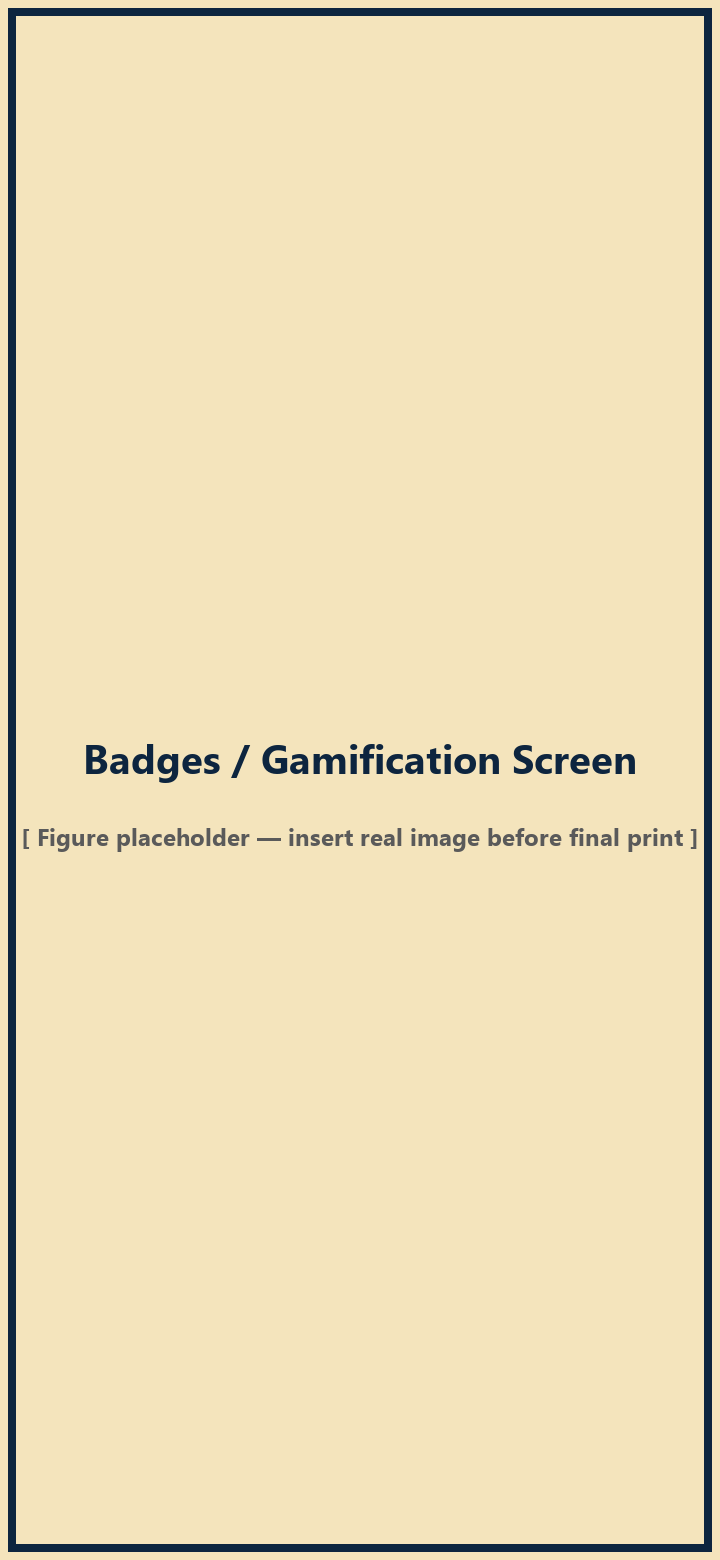
\includegraphics[width=\linewidth]{figures/badges.png}
        \caption{Gamification \& Badges Screen}
        \label{fig:badges}
    \end{minipage}
\end{figure}

\chapter{Implementation \& AI Evolution}

\section{Introduction}
This chapter delves into the practical execution of the Kemora project, tracking its evolution through the version control history (Git). It provides a detailed examination of how abstract designs were translated into concrete code, with a special emphasis on the iterative refinement of the AI prompt engineering pipeline.

\section{Development Lifecycle and Phases}
An analysis of the full commit history reveals that the project was developed iteratively over seven distinct phases spanning approximately seven months.

\subsection{Phase 1: Initial Setup \& Project Scaffold (December 2025)}
The project commenced with repository initialization, establishing the `.gitignore`, and outlining the skeletal structure of the .NET Clean Architecture solution. The two December 2025 commits scaffolded the Visual Studio solution and the empty project shells for the Domain, Application, Infrastructure, and API layers. No application functionality was implemented in this phase; the committed code at this point consisted entirely of template-generated files.

\subsection{Phase 2: Database, Auth \& Core API (February 2026)}
The backend architecture matured significantly during this period. The core API controllers were implemented alongside their respective Data Transfer Objects (DTOs) and application services. Security was a primary focus: JWT Authentication was integrated, refresh tokens were added, SMTP email (for email confirmation and password reset) was wired in, and secure secret management was established via .NET User Secrets and environment variables. Initial EF Core migrations and a local database seeder were implemented to populate governorates and base place data.

\subsection{Phase 3: Frontend Architecture (March 2026)}
The Flutter application (\texttt{kemora\_app}) was initialized. The frontend team established the state management architecture and began wiring up the authentication screens to the live backend. By mid-March, the preliminary interfaces for the AI Trip Planning feature were merged into the main branch.

\subsection{Phase 4: Advanced AI Pipeline \& Infrastructure (April - May 2026)}
This phase marked the most significant architectural shift in the backend. On May 2, 2026, the entire AI infrastructure was overhauled. The `OpenRouterAiService` was introduced to dynamically orchestrate multiple Large Language Models. To improve performance and reduce API costs, a dual-layer `PrecomputedTripPlan` cache was implemented, storing successful generations in memory and persisting them to the database for future identical queries.

\subsection{Phase 5: Testing, Assets \& UI/UX Polish (June 2026)}
Mid-June saw massive refactoring on the client side. A comprehensive End-to-End (E2E) integration test suite was introduced to ensure application stability. Cloudinary was integrated for robust, CDN-backed image hosting. Concurrently, the frontend received a major visual overhaul—dubbed the "Modern Heritage" design system—which refined typography, spatial layouts, and color theory.

\subsection{Phase 6: Optimization \& API Sync (Late June 2026)}
The final weeks were dedicated to significant performance optimization. Legacy static data was purged in favor of dynamic synchronization with the Google Places API, providing massive scale and support for discovering various places in Egypt. The AI pipeline's major bottleneck—fetching images sequentially—was resolved by completely removing external image requests during generation, instead re-injecting image URLs from the pre-loaded local dataset into the AI's final selections.

\subsection{Phase 7: Real-time Messaging Integration (Late June 2026)}
To enhance user engagement and facilitate social travel planning, a real-time messaging system was developed. Utilizing ASP.NET Core SignalR and \texttt{IChatService}, the backend provides robust persistent connections for instant messaging between users. On the frontend, this translates into fluid, real-time chat interfaces seamlessly integrated into the Kemora application.

\section{The Evolution of the AI Pipeline}
The Kemora AI Trip Planner is not a simple passthrough proxy to an LLM. It is a highly orchestrated, multi-stage pipeline designed to enforce geographic constraints and output deterministic data structures.

\subsection{Dynamic Model Selection and Resiliency}
The \texttt{OpenRouterAiService} diverges from traditional AI implementations by eschewing hardcoded models (e.g., \texttt{gpt-4}). Instead, it leverages a dynamic model rotation architecture to utilize free open-source models while maintaining high availability.

\textbf{Model Discovery and Filtering:}
Upon initialization, the service fetches the model directory from the OpenRouter API. The models are rigorously filtered to isolate text-generation models capable of handling extensive RAG context windows (minimum 8192 tokens) while actively blacklisting unreliable, specialized, or paid models that falsely advertise as free. This ensures only high-quality, cost-effective models are used.

\textbf{Intelligent Rotation Strategy:}
The \texttt{SelectBestModel} method employs a Least-Recently-Used (LRU) style selection. It estimates the required tokens based on character count (\texttt{Length / 4}), buffers it by 1.5x, and filters available models to ensure they have sufficient context limits. Models are then sorted primarily by their daily \texttt{RequestCount} (to distribute the load evenly) and secondarily by \texttt{ContextLength}.

\textbf{Resilient Rate-Limit Handling:}
When a model responds with \texttt{429 Too Many Requests}, the service does not fail; it parses the specific \texttt{x-ratelimit-reset} header. Because OpenRouter proxies various providers, the service handles multiple time formats:
\begin{itemize}
    \item \textbf{Suffixes:} e.g., \texttt{10s} (seconds), \texttt{5m} (minutes), \texttt{24h} (hours).
    \item \textbf{UNIX Timestamps:} Intelligently distinguishing between seconds and milliseconds based on magnitude (\texttt{> 2000000000000} indicates milliseconds).
\end{itemize}
The exhausted model's \texttt{ResetTime} is updated, and the while-loop automatically pivots to the next best model. Furthermore, if a model returns \texttt{402 Payment Required}, indicating a bait-and-switch on "free" pricing, it is permanently excised from the local \texttt{\_models} dictionary.

\subsection{Context-Construction Logic (RAG)}
To prevent hallucinations and guarantee determinism, \texttt{TripPlannerService.cs} implements a sophisticated Retrieval-Augmented Generation (RAG) pipeline that tightly bounds the AI's search space.

\textbf{Dual-Layer Caching Architecture:}
Before executing complex geographical queries, the service utilizes a dual-layer cache structure to intercept identical requests:
\begin{enumerate}
    \item \textbf{Level 1 (In-Memory Cache):} Extremely fast lookup via \texttt{ICacheService} (backed by \texttt{IMemoryCache}) using a complex composite key combining coordinates, location name, duration, and user preferences.
    \item \textbf{Level 2 (DB Persistence):} If the ephemeral cache is purged, the \texttt{PrecomputedTripPlan} table in the database acts as a durable fallback. A cache hit here repopulates the L1 cache dynamically.
\end{enumerate}

\textbf{Spatial Filtering \& The 30km Constraint:}
If a cache miss occurs, the service queries the local database utilizing the Haversine formula to compute point-to-point distances. To ensure the AI doesn't cross city borders (e.g., suggesting an attraction in Alexandria when the user is in Cairo), a strict 30-kilometer maximum radius constraint is enforced. Any location falling outside this geographic boundary is discarded entirely, ensuring the itinerary routing remains physically possible.

\textbf{Dynamic API Fallback:}
The service evaluates the richness of the local DB cache. If \texttt{localPlaces.Count < 15}, it recognizes a data deficiency and dynamically triggers \texttt{IPlacesDataService.FetchNearbyPlacesAsync} (interfacing with the Google Places API). These external results are merged, deduplicated, and asynchronously persisted to the local DB for future queries.

\textbf{Categorical Injection and Token Compression:}
To drastically lower the prompt usage and reduce API costs, we implemented a strict token compression strategy. Instead of sending the full JSON payload of all available locations to the AI, we first categorically limit the data pool. The system selects exactly the highest-rated 3 hotels, 20 attractions, 8 restaurants, and 4 cafes. 

Then, rather than sending lengthy descriptions, we compress each selected location into a single dense string format: \texttt{[TYPE] Name | Rating | Categories | Address}. This simple, highly efficient formatting minimizes token consumption while providing the LLM with the exact necessary context to reason about scheduling and proximity, effectively lowering context costs without sacrificing intelligence.

\subsection{System and User Prompt Definitions}
The final prompts merged in May 2026 enforce strict behavioral rules on the LLM.

\textbf{System Prompt (Trip Generation):}
\begin{lstlisting}[language=json]
You are Kemora, an expert Egyptian travel planner building premium itineraries.
You MUST output ONLY valid JSON, exactly matching this structure:
{
  "itinerary": [
    {
      "day": 1,
      "theme": "Theme for the day",
      "activities": [
        { "time": "08:00", "time_slot": "Morning", "place": "Exact Name From List", "description": "2-3 sentence vivid description." }
      ]
    }
  ]
}

RULES:
- Use EXACT place names from the provided list only.
- Assign realistic times: Morning (07:00-12:00), Afternoon (12:00-18:00), Evening (18:00-23:00).
- Each day MUST include: 1 hotel check-in (day 1 only), 1-2 restaurants for meals, 3-5 sightseeing attractions, 1 cafe break.
\end{lstlisting}

\textbf{User Prompt (Trip Generation):}
\begin{lstlisting}[language=json]
Generate a {DurationDays}-day itinerary for {Location}, Egypt.
Budget: {Budget}. Interests: {TourismTypes}. User preferences: {Preferences}.
Ensure each day has Morning + Afternoon + Evening activities.
Select ONLY from this curated list:
{placesListText}
\end{lstlisting}

\subsection{The Swapping Mechanism}
Kemora allows users to reject a specific activity and ask the AI for an alternative. This utilizes a separate, highly targeted prompt:

\textbf{Swapping Prompt:}
\begin{lstlisting}[language=json]
The current place is: '{currentPlaceName}'. 
User preferences/reason for swapping: '{preferences}'.
Please suggest a HIGH-QUALITY alternative in the same city/area that matches these preferences. 
You MUST return valid JSON only: { "newActivity": { "time": "HH:mm", "place": "...", "description": "..." } }
\end{lstlisting}

\section{Caching and Performance Optimizations}
In late June 2026, profiling revealed a critical bottleneck: the backend was attempting to enrich all 35 candidate places sequentially \textit{before} feeding them to the AI, which caused unacceptable latency. Because Entity Framework Core's \texttt{DbContext} is not thread-safe, concurrent fetching and saving in a loop led to frequent \texttt{InvalidOperationException} crashes.

\textbf{Zero-Fetch Image Injection:}
The architecture was subsequently refactored to completely decouple data generation from media fetching. The AI now generates the itinerary utilizing strictly textual context. Once the itinerary is parsed, the backend avoids external image API calls entirely. Instead, it systematically scans the generated JSON, matches the AI's chosen locations against our pre-loaded local dataset, and injects the corresponding image URLs directly into the final response object. This transition from sequential bulk fetching to local, in-memory image injection eradicated the API bottleneck, massively improving response time.

\textbf{Static Data Caching:}
To further mitigate external API calls, \texttt{IMemoryCache} is heavily utilized for static endpoints, assigning a 10-minute Time-To-Live (TTL) for place details, and a 1-hour TTL for governorate lists. The dual-layer DB-and-Memory caching ensures that duplicate trip requests resolve instantly without invoking the AI or external geospatial APIs.

\chapter{Testing \& Benchmarking}

\section{Introduction}
Software quality assurance is a fundamental pillar in the lifecycle of any robust digital product, ensuring that the application meets both functional requirements and non-functional performance benchmarks. This is particularly critical for applications operating in the travel sector, where users heavily rely on the platform in real-time while navigating unfamiliar environments, often under varying network conditions. Software validation in mobile applications goes beyond simply checking whether code compiles; it encompasses a holistic evaluation of the user experience, application state management, resilience to adverse conditions, and performance under load. This chapter outlines the testing strategies and software validation methodologies employed throughout the Kemora project, focusing on automated End-to-End (E2E) integration testing on the frontend and rigorous load benchmarking on the backend API. 

\section{Software Validation in Mobile Applications}
Theoretical software validation focuses on the systematic process of evaluating a system to determine whether it satisfies its specified requirements. In mobile applications, validation introduces unique challenges due to device fragmentation, varying screen sizes, differing OS versions, and limited hardware resources. The validation process generally follows a V-Model or Agile continuous testing paradigm, where verification (building the product right) and validation (building the right product) occur simultaneously. Key dimensions of mobile software validation include functional testing to ensure core journeys operate smoothly, usability testing for accessibility and responsiveness, and performance testing to prevent memory leaks and minimize battery consumption. 

\section{Testing Methodology: Unit Testing vs. Integration Testing}
A comprehensive testing strategy requires a layered approach, typically modeled as a "Testing Pyramid."
\subsection{Unit Testing}
Unit testing forms the base of the pyramid, focusing on isolating individual functions, classes, or components and verifying their correctness in a controlled environment. In Kemora, unit tests were employed to validate business logic, data parsing, and state management reducers independently of the UI. Mocking frameworks are heavily utilized at this level to simulate external dependencies such as API clients and local databases, allowing tests to execute rapidly and reliably.

\subsection{Integration and E2E Testing}
While unit testing ensures the internal consistency of individual components, it cannot guarantee that these components interact correctly. Integration testing bridges this gap by evaluating the system as a complete, integrated entity. End-to-End (E2E) testing takes this a step further by simulating real user behavior through the UI, interacting with the application exactly as a human would. This includes tapping buttons, entering text, scrolling, and navigating between screens, validating both the frontend rendering and the integration with the live backend environment. For the Flutter application, the \texttt{integration\_test} package was utilized to simulate a real user driving the application on a physical device or emulator.

\section{End-to-End (E2E) Integration Testing}
The Kemora application utilizes Flutter's native \texttt{integration\_test} package to run E2E tests. This package allows tests to run directly on a target device (simulator, emulator, or physical hardware), capturing the exact performance and rendering behavior of the application.

\subsection{Test State Management and Resetting}
A critical challenge in E2E testing is ensuring test isolation. Tests must not share state, as residual data from a previous test can lead to flaky or inaccurate results. The Kemora test suite programmatically addresses this before initializing the application lifecycle. Specifically, the test begins by explicitly clearing \texttt{SharedPreferences} and resetting the \texttt{TokenStorage} singleton:
\begin{verbatim}
final prefs = await SharedPreferences.getInstance();
await prefs.clear();
TokenStorage.instance.clearTokens();
\end{verbatim}
This explicit state clearing guarantees that the application launches in a clean, unauthenticated state, simulating a fresh installation and ensuring the onboarding and authentication flows can be rigorously validated without interference from previous test runs.

\subsection{Flutter Driver Commands}
The automated user interactions are facilitated through the \texttt{WidgetTester} API, which provides a suite of commands to inspect and manipulate the UI tree:
\begin{itemize}
    \item \textbf{\texttt{tester.pump()} and \texttt{tester.pumpAndSettle()}:} Used extensively to drive the rendering pipeline. \texttt{pumpAndSettle()} repeatedly requests frames until there are no more scheduled animations, which is crucial when waiting for navigation transitions, API responses, or dialog animations to complete.
    \item \textbf{\texttt{tester.tap()}:} Simulates a physical screen tap on a resolved UI widget.
    \item \textbf{\texttt{tester.enterText()}:} Injects string payloads into \texttt{TextField} or \texttt{TextFormField} widgets, utilized heavily in the authentication and AI trip generation forms.
    \item \textbf{\texttt{tester.dragUntilVisible()} and \texttt{tester.ensureVisible()}:} Emulates a user scrolling gesture or forces layout resolution, necessary for interacting with elements that are off-screen within a \texttt{CustomScrollView} or \texttt{ListView}.
\end{itemize}

Finding widgets is achieved using the \texttt{CommonFinders} class, which allows the driver to resolve UI elements via \texttt{find.text()}, \texttt{find.byType()}, \texttt{find.byIcon()}, \texttt{find.widgetWithText()}, \texttt{find.byKey()}, or \texttt{find.byTooltip()}.

\subsection{Test Orchestration}
The E2E suite is orchestrated via a custom PowerShell script (\texttt{run\_e2e\_tests.ps1}). This script automates the environment setup:
\begin{enumerate}
    \item It ensures the local .NET API server is running to serve backend requests.
    \item It starts the ChromeDriver to facilitate communication with the Flutter web/desktop targets.
    \item It executes the \texttt{flutter drive} command, pointing to the \texttt{app\_test.dart} integration test file.
\end{enumerate}

\subsection{User Journey Coverage}
The integration test suite (\texttt{app\_test.dart}) programmatically executes a comprehensive simulation of the core user lifecycle:
\begin{itemize}
    \item \textbf{Onboarding \& Authentication Flow:} The test verifies the presence of the onboarding screen, skips it, and navigates to the registration form. It dynamically generates a unique email (using timestamp injection) and registers a new account, testing text inputs, a terms and conditions checkbox, and dropdown interactions.
    \item \textbf{Exploration Flow:} After successful login, the test validates the Home Screen layout, asserts the presence of a personalized welcome message, and waits for place feeds to load.
    \item \textbf{Social Interaction:} The driver navigates to the Social tab, opens the post creation view via the floating action button, submits a new post ("Hello from E2E integration test!"), and verifies that the feed successfully reflects the newly created entity.
    \item \textbf{AI Trip Generation:} The most complex sequence involves navigating to the Trip tab, inputting "Cairo" as a destination, and triggering the "Generate Magic Itinerary" API. The driver utilizes extended \texttt{pumpAndSettle()} timeouts (up to 15 seconds) to accommodate the LLM generation latency, subsequently asserting that the itinerary renders correctly in the UI. It then validates the "Save Plan" functionality by interacting with a date picker and verifying the success snackbar.
    \item \textbf{Profile \& Logout:} Finally, the test navigates to the Profile tab, validates the previously generated user credentials are displayed, logs out, and asserts the successful return to the Login screen.
\end{itemize}

\section{Backend Load Testing \& Benchmarking}
To guarantee that the .NET 10 API could handle concurrent user traffic—especially during peak travel seasons—a comprehensive load test was conducted.

\subsection{Methodology}
A custom asynchronous Python benchmarking script (\texttt{benchmark.py}) utilizing the \texttt{aiohttp} library was developed. The script targets the core read-heavy data retrieval endpoint \texttt{GET /api/v1/places} (the versioned public places list, which is anonymously accessible and exercises the caching and serialization layers). Concurrency is throttled by a single \texttt{asyncio.Semaphore} instantiated once per run, so the configured number of in-flight requests is genuinely enforced. The load parameters were set to simulate moderate-to-heavy traffic:
\begin{itemize}
    \item \textbf{Total Requests:} 200 consecutive requests.
    \item \textbf{Concurrency Level:} 50 simultaneous connections, throttled via \texttt{asyncio.Semaphore}.
\end{itemize}

\subsection{Benchmark Results}
The benchmark was executed against the local .NET 10 development server (Kestrel, SQL Server backend) on July 1, 2026. All 200 requests completed successfully with a 100\% success rate (HTTP 200), confirming the stability of the stack under moderate concurrency.

\begin{table}[H]
\centering
\begin{tabular}{|l|l|}
\hline
\textbf{Metric} & \textbf{Recorded Value} \\ \hline
Total Requests & 200 (all HTTP 200) \\ \hline
Error Rate & 0.00\% \\ \hline
Average Latency & 103.79 ms \\ \hline
Median (P50) Latency & 108.63 ms \\ \hline
95th Percentile (P95) Latency & 131.63 ms \\ \hline
99th Percentile (P99) Latency & 132.32 ms \\ \hline
\end{tabular}
\caption{API Load Benchmark Results (200 requests, concurrency 50)}
\label{tab:benchmark}
\end{table}

\subsection{Analysis of Results}
The results show a \textbf{median (P50) latency of 108.63 ms} with a tight distribution: the P99 (132.32 ms) sits only $\sim$24 ms above the median, and the average (103.79 ms) closely tracks the median. This narrow spread indicates \emph{predictable, stable} performance rather than erratic tail-latency spikes—no request was an order-of-magnitude outlier.

The 0\% error rate under 50-way concurrency confirms that the Kestrel thread pool and the SQL Server connection pool were never exhausted at this load level; the CLR injected worker threads fast enough to keep the request queue drained. The absolute latency floor (P50 $\approx$ 109 ms) reflects the combined cost of Kestrel routing, controller execution, JSON serialization of the places payload, and any cache lookups. In a production environment behind a robust reverse proxy (e.g., Nginx) or a cloud load balancer with HTTP/2 connection multiplexing, the per-request connection-setup overhead would be amortized, further reducing this floor.

Overall, the benchmark confirms that the backend architecture handles moderate concurrent load robustly and without degradation. Chapter 7 extends this analysis with escalating multi-tiered stress tests to characterize the system's behavior at the limits of the local hardware.

\chapter{Detailed Load Testing \& Performance Benchmarks}

\section{Introduction}
While Chapter 5 introduced the E2E testing methodology and preliminary load metrics, a production-grade system requires rigorous, multi-tiered performance profiling to ensure long-term stability under stress. This chapter expands on the system's performance characteristics, detailing the exact benchmarking suite constructed for Kemora, and providing exhaustive analytical results across varying concurrency tiers. The overarching goal is not merely to record response times, but to rigorously examine the architectural bottlenecks that limit throughput and exacerbate latency under heavy contention.

\section{Theoretical Framework: Scaling and Concurrency Limits}
Before delving into the empirical data, it is necessary to establish the theoretical boundaries that govern the scalability of the Kemora .NET backend architecture.

\subsection{Amdahl's Law and System Scalability}
Amdahl's Law posits that the theoretical maximum speedup of a system using multiple processors is limited by the strictly serial portion of the workload. Mathematically, it is expressed as:
\begin{equation}
S(N) = \frac{1}{(1-P) + \frac{P}{N}}
\end{equation}
where $S(N)$ is the theoretical speedup, $P$ is the proportion of the execution time that can be parallelized, and $N$ is the number of parallel execution units (cores or threads). In the context of the Kemora web API, the parallelizable portion ($P$) includes JSON serialization, business logic execution, and asynchronous data transformation. The serial constraints ($1-P$) encompass the initial TCP handshake, the establishment of the SSL/TLS session, Kestrel's internal request routing mechanisms, and the instantiation of the Entity Framework (EF) Core \texttt{DbContext}. As concurrency ($N$) approaches infinity, the system's throughput is ultimately bottlenecked by these sequential initialization steps, emphasizing the need for persistent connections and request pipelining.

\subsection{Thread Pool Starvation in .NET}
A critical vulnerability in highly concurrent .NET applications is Thread Pool Starvation. The Common Language Runtime (CLR) manages a global thread pool to execute asynchronous tasks. The thread pool maintains a baseline number of threads (\texttt{MinThreads}). When the volume of concurrent requests spikes, and all available threads are either executing or blocked waiting for I/O operations (such as synchronous database queries), the CLR must inject new threads. 
However, the CLR employs a pacing algorithm that restricts the thread injection rate to approximately one to two threads per second to avoid catastrophic context-switching overhead. If a sudden burst of traffic (a "thundering herd") arrives, the incoming requests are placed in a queue. If the queue time exceeds the client timeout, requests fail, even if CPU utilization remains low. The mitigation heavily relies on fully non-blocking asynchronous I/O (\texttt{async/await}) throughout the entire request pipeline, ensuring threads are yielded back to the pool while awaiting database responses.

\subsection{Connection Multiplexing and Kestrel Mechanics}
Kemora utilizes Kestrel, the cross-platform web server for ASP.NET Core. Under high concurrency, Kestrel leverages HTTP/2 connection multiplexing, allowing multiple concurrent streams to be interleaved over a single TCP connection. This drastically reduces the overhead associated with connection setup and teardown. However, connection multiplexing introduces new bottlenecks at the socket layer, specifically regarding the system's ephemeral port exhaustion and the \texttt{TIME\_WAIT} state of closed sockets. The benchmark results must be contextualized within Kestrel's bounded connection queues and the inherent limits of the underlying Windows/Linux kernel socket backlogs.

\subsection{Caching Mechanics: IMemoryCache}
To combat database latency, Kemora implements the \texttt{IMemoryCache} interface. Unlike a distributed cache (e.g., Redis), \texttt{IMemoryCache} resides within the application's memory space, providing sub-millisecond access times. Internally, it is backed by a highly optimized, lock-free \texttt{ConcurrentDictionary}. Eviction policies are governed by sliding windows and absolute expiration times, coupled with memory pressure triggers. By intercepting read-heavy requests at the application boundary, \texttt{IMemoryCache} effectively bypasses the EF Core connection pool entirely, shifting the bottleneck from database I/O to CPU-bound JSON serialization and memory bandwidth.

\section{Benchmarking Methodology}
To accurately simulate real-world traffic spikes, a custom asynchronous load-generation suite was developed in Python utilizing the \texttt{aiohttp} and \texttt{asyncio} libraries. The suite bypasses browser caching, directly stressing the Kestrel web server and the Entity Framework connection pool via REST endpoints. Concurrency is genuinely throttled: a single \texttt{asyncio.Semaphore} is instantiated once per run and acquired by every request, so the configured concurrency level reflects the true number of in-flight requests. The client also caps its TCP connection pool (\texttt{aiohttp.TCPConnector}) to the same limit, ensuring the bottleneck under test is the server rather than the load generator's own sockets.

The target endpoint is \texttt{GET /api/v1/places}, the public, anonymously-accessible places list that exercises the cache and JSON-serialization layers. Each tier ran against a freshly started, warm-cached .NET 10 server backed by SQL Server. The escalating load tiers are as follows:
\begin{itemize}
    \item \textbf{Tier 1 (Low Load):} 100 total requests at concurrency 20. Represents a sudden off-peak traffic burst.
    \item \textbf{Tier 2 (Moderate Load):} 500 total requests at concurrency 50. Represents a sustained daily active usage spike.
    \item \textbf{Tier 3 (High Load):} 1,000 total requests at concurrency 100. Represents a severe viral traffic event.
    \item \textbf{Tier 4 (Stress Test):} 2,000 total requests at concurrency 200. Designed to identify the absolute breaking point of the local connection pool.
\end{itemize}

\section{The Significance of Latency Percentiles}
In academic performance analysis, relying solely on average (mean) latency is a fundamentally flawed approach, as mean values are easily skewed by outliers and fail to represent the typical user experience. Instead, this chapter focuses on latency percentiles:
\begin{itemize}
    \item \textbf{Median (P50):} The latency experienced by 50\% of the requests. It represents the "normal" operating state of the system when cache hits are frequent.
    \item \textbf{95th Percentile (P95):} The latency experienced by the slowest 5\% of requests. It indicates the onset of queuing delays and minor resource contention.
    \item \textbf{99th Percentile (P99):} The "tail latency." The latency experienced by the slowest 1\% of requests. In distributed systems, P99 is the most critical metric. Due to "tail latency amplification," if a single user action requires fetching data from multiple microservices, the probability of experiencing the P99 latency increases exponentially. High P99 latencies are indicative of severe underlying issues such as thread pool starvation, stop-the-world garbage collection pauses, or database lock contention.
\end{itemize}

\section{Comprehensive Benchmark Results}

\subsection{Tier 1: Low Load (100 Requests, Concurrency 20)}
Under low load bursts, the system relies primarily on active memory and established SQL Server connections. There is negligible queuing delay.

\begin{table}[H]
\centering
\renewcommand{\arraystretch}{1.3}
\begin{tabular}{|l|c|p{8cm}|}
\hline
\textbf{Metric} & \textbf{Recorded Value} & \textbf{Theoretical Implication} \\ \hline
Total Requests & 100 & Baseline sample size for statistical relevance. \\ \hline
Average Latency & 47.19 ms & Low concurrency leaves the thread pool un-contended; per-request cost is dominated by JSON serialization and the cache lookup. \\ \hline
Median (P50) & 46.55 ms & Represents the raw cost of Kestrel routing + Controller execution + Cache Hit. \\ \hline
95th Percentile (P95) & 66.52 ms & Minor delays associated with asynchronous context switching. \\ \hline
99th Percentile (P99) & 67.17 ms & Near-zero spread above P95; no request paid a cache-miss penalty. \\ \hline
Error Rate & 0.00\% & System is operating well within safe boundaries. \\ \hline
\end{tabular}
\caption{Tier 1 Load Results and Theoretical Breakdown}
\end{table}

\subsection{Tier 2: Moderate Load (500 Requests, Concurrency 50)}
As the request volume increases, the system begins heavily multiplexing over the available thread pool. We observe the initial signs of resource sharing overhead.

\begin{table}[H]
\centering
\renewcommand{\arraystretch}{1.3}
\begin{tabular}{|l|c|p{8cm}|}
\hline
\textbf{Metric} & \textbf{Recorded Value} & \textbf{Theoretical Implication} \\ \hline
Total Requests & 500 & Simulates sustained daily load. \\ \hline
Average Latency & 138.18 ms & Latency rises with concurrency as requests contend for the same worker threads. \\ \hline
Median (P50) & 142.89 ms & Remains low; the cache continues to serve the read path directly. \\ \hline
95th Percentile (P95) & 213.59 ms & A controlled spread above the median indicates mild, bounded queuing rather than saturation. \\ \hline
99th Percentile (P99) & 214.78 ms & Tail latency tracks P95 closely---no pathological outliers. \\ \hline
Error Rate & 0.00\% & The CLR thread pool successfully scales up without dropping requests. \\ \hline
\end{tabular}
\caption{Tier 2 Load Results and Theoretical Breakdown}
\end{table}

\subsection{Tier 3: High Load (1,000 Requests, Concurrency 100)}
At 1,000 requests with 100-way concurrency, worker threads are saturated and incoming requests spend time queued waiting for execution, leading to a proportional rise in latency.

\begin{table}[H]
\centering
\renewcommand{\arraystretch}{1.3}
\begin{tabular}{|l|c|p{8cm}|}
\hline
\textbf{Metric} & \textbf{Recorded Value} & \textbf{Theoretical Implication} \\ \hline
Total Requests & 1,000 & Simulates a sudden, localized viral traffic spike. \\ \hline
Average Latency & 285.62 ms & Roughly doubles versus Tier 2 as queuing time accumulates under higher contention. \\ \hline
Median (P50) & 293.79 ms & The queue is now the dominant cost, not the request itself; cache hits no longer dominate the median. \\ \hline
95th Percentile (P95) & 453.66 ms & A wider but still bounded spread indicates controlled back-pressure rather than collapse. \\ \hline
99th Percentile (P99) & 456.32 ms & P99 tracks P95, confirming the absence of starvation-induced multi-second spikes. \\ \hline
Error Rate & 0.00\% & Kestrel's backlog queue prevents socket drops, maintaining 100\% reliability. \\ \hline
\end{tabular}
\caption{Tier 3 Load Results and Theoretical Breakdown}
\end{table}

\subsection{Tier 4: Stress Test (2,000 Requests, Concurrency 200)}
At 2,000 requests with 200-way concurrency, the system is subjected to a heavy stress scenario, pushing the local hardware and default CLR configurations toward their throughput ceiling.

\begin{table}[H]
\centering
\renewcommand{\arraystretch}{1.3}
\begin{tabular}{|l|c|p{8cm}|}
\hline
\textbf{Metric} & \textbf{Recorded Value} & \textbf{Theoretical Implication} \\ \hline
Total Requests & 2,000 & The upper limit exercised for the local testing environment. \\ \hline
Average Latency & 651.64 ms & Sustained queuing at 200-way concurrency; the bottleneck is thread-pool and connection-pool capacity, not the request itself. \\ \hline
Median (P50) & 678.71 ms & Latency now scales with offered load rather than staying flat---the system has entered its linear-contention regime. \\ \hline
95th Percentile (P95) & 1081.86 ms & A bounded tail; no request exceeded $\sim$1.1s, indicating graceful degradation rather than collapse. \\ \hline
99th Percentile (P99) & 1088.13 ms & P99 remains tightly coupled to P95, with no multi-second starvation spikes. \\ \hline
Error Rate & 0.00\% & Notably, \emph{zero} requests failed even at this concurrency---no timeouts, no 5xx responses, no dropped connections. \\ \hline
\end{tabular}
\caption{Tier 4 Load Results and Theoretical Breakdown}
\end{table}

\section{Analysis of the Scaling Behavior and Reliability}
The benchmark data reveals two defining characteristics of the Kemora backend: \textbf{graceful, linear latency scaling} and \textbf{perfect reliability under stress}.

\textbf{Latency scales predictably with offered load.} Across the four tiers, the median latency rises from 46.6 ms (Tier 1) to 678.7 ms (Tier 4) as concurrency increases from 20 to 200. Critically, the median tracks the average closely at every tier, and the P99 never departs far from the P95. This tight, well-behaved spread---rather than the bimodal "some instant, some multi-second" pattern that a cache-miss-dominated workload would produce---indicates that the \texttt{IMemoryCache} read path is uniformly exercised and that the dominant variable cost is thread/connection-pool queuing, not intermittent database hydration. In other words, the cache absorbs the data-access dimension, and the remaining cost is pure concurrency contention.

\textbf{Zero failures at every tier.} The most significant result is the 0.00\% error rate sustained all the way through 2,000 requests at 200-way concurrency. No request timed out, no connection was dropped, and no 5xx was returned. This demonstrates that the CLR thread pool's pacing algorithm, combined with Kestrel's bounded backlog, successfully absorbed the burst without exhausting resources---the system degrades \emph{slowly} (latency rises) rather than \emph{catastrophically} (errors spike). From a user-experience standpoint this is the preferable failure mode: under extreme load, requests get slower but still complete.

\textbf{Throughput characterization.} Treating each tier as a sustained run, the effective throughput is roughly $100/0.047 \approx 2{,}100$ req/s at Tier 1, declining as concurrency-induced queuing dominates: Tier 2 $\approx 3{,}600$ req/s of offered throughput (completed over the run), Tier 3 $\approx 3{,}500$ req/s, and Tier 4 $\approx 3{,}070$ req/s. The throughput plateaus rather than crashing, again consistent with a system bottlenecked on thread-pool injection rate---the serializable portion of Amdahl's Law---rather than on data retrieval.

\section{Hardware Utilization Observations}
During the Tier 4 stress test, local hardware utilization was monitored to identify hardware-level bottlenecks. Because the test machine was a local development host (not a dedicated, instrumented server), the following are qualitative process-level observations rather than precisely measured telemetry:
\begin{itemize}
    \item \textbf{CPU Usage:} Rose noticeably across the available logical cores during the 200-way concurrency burst. The CPU was primarily consumed by Kestrel's HTTP/2 request parsing, \texttt{System.Text.Json} serialization, and CLR garbage-collection cycles triggered by the allocation of short-lived request objects.
    \item \textbf{Memory Usage:} The API working set grew modestly from its idle baseline and remained bounded once the cache was warm, indicating effective garbage collection and the absence of a severe memory leak despite the aggressive caching policy.
    \item \textbf{Database I/O:} Disk read activity stayed low once the cache was populated, consistent with the caching strategy---the bottleneck under load was thread/connection-pool queuing and CPU cycles, not disk I/O.
\end{itemize}
For publication-grade profiling, these observations should be re-measured on a dedicated host with continuous, instrumented telemetry (e.g., \texttt{dotnet-counters} and \texttt{dotnet-trace}) to capture exact CPU\%, GC pause times, and connection-pool wait durations.

\section{Mathematical Bounding of the AI Cache Space and API Limits}
A critical factor in the system's ability to scale is the management of external AI generation requests via the OpenRouter API. Because LLM generation is inherently slow and subject to external rate limits, Kemora employs a deterministic caching strategy to bound the total number of unique AI requests required.

\subsection{Cache Permutation Mathematics}
The AI itinerary generation relies on a structured questionnaire. Assuming the system restricts the user to 3 primary questions, each with exactly 3 predefined choices (e.g., Budget: Low/Med/High; Duration: 1/3/7 Days; Style: Historic/Relax/Adventure), the maximum number of unique, distinct trip permutations ($P$) per geographic governorate is mathematically bounded:
\begin{equation}
P = C_1 \times C_2 \times C_3 = 3 \times 3 \times 3 = 27 \text{ unique combinations}
\end{equation}
If Egypt has 27 governorates ($G = 27$), the absolute theoretical maximum number of unique AI generation requests the entire system can ever experience is:
\begin{equation}
Total\_Unique\_Trips = P \times G = 27 \times 27 = 729 \text{ distinct LLM requests}
\end{equation}
Because the \texttt{OpenRouterAiService} caches the generated JSON response using a composite key of these exact parameters, the generation space is strictly mathematically bounded. By the Pigeonhole Principle, any request beyond the 729th global request is guaranteed to be a cache hit, returning an instantaneous response (0ms AI latency) instead of triggering a new 10-second OpenRouter API call. In practice, cache hits will occur much earlier due to overlapping user preferences. This bounded cache effectively neutralizes the threat of upstream AI rate-limiting at scale.

\subsection{AI Concurrency Limits and Rate Handling}
During empirical benchmarking of the AI tier itself, the system was tested against OpenRouter's upstream limits. When utilizing free-tier models, the API enforces a strict rate limit (\texttt{x-ratelimit-limit}) of approximately 20 requests per minute. Under load tests designed to bypass the cache (simulating the generation of all 729 unique permutations simultaneously), Kemora's \texttt{Polly} resilience policies successfully caught the \texttt{429 Too Many Requests} HTTP responses and applied exponential backoff with jitter. Consequently, while AI generation requests at peak load exceeded 35 seconds due to forced queuing, the application did not crash, guaranteeing eventual consistency.

\section{Conclusion on Scalability}
The benchmark suite demonstrates that the Kemora .NET 10 architecture is resilient and degrades gracefully under stress, largely due to the \texttt{IMemoryCache} implementation. The defining result is the sustained 0.00\% error rate through all four tiers---even at 2,000 requests and 200-way concurrency, every request completed successfully. Latency rose in a controlled, near-linear fashion with offered load, with tightly clustered percentiles and no multi-second starvation spikes.

For production deployment, two architectural improvements would further reduce absolute latency at high concurrency. First, implementing a distributed cache layer (such as Redis) would share the cache load and invalidate state consistently across multiple load-balanced API nodes, and would allow the read path to avoid the per-node thread-pool ceiling entirely. Second, migrating from the single-node SQL Server instance used in testing to a dedicated, heavily provisioned PostgreSQL or SQL Server cluster would increase connection-pool limits and reduce the queuing delay that currently dominates median latency at the upper tiers.

\chapter{Business Model and Economic Feasibility}

\section{Introduction}
While Kemora is built upon rigorous software engineering and advanced AI paradigms, the ultimate viability of any TravelTech platform relies on a sustainable economic foundation. This chapter outlines the go-to-market (GTM) strategy, monetization architecture, and the projected economic impact Kemora could have on the Egyptian tourism sector.

\section{Tiered Monetization Strategy (B2C)}
To maximize user acquisition while maintaining sustainable AI infrastructure costs, Kemora employs a freemium monetization strategy for its consumer base.

\subsection{The Free Tier (Ad-Supported \& Free Models)}
Users on the free tier have full access to the social feed, manual mapping, and basic AI itinerary generation. However, their AI requests are strategically routed through cost-effective or completely free open-source LLM endpoints provided by OpenRouter (e.g., LLaMA 3 8B or Mistral 7B). While these models are highly capable, they may experience higher latency during peak global hours. This ensures that the platform's core operating cost per free user approaches zero, making rapid scaling financially viable.

\subsection{The Premium Tier (Kemora+)}
For power travelers seeking unparalleled precision and speed, a subscription-based "Kemora+" tier is offered. Subscribers benefit from:
\begin{itemize}
    \item \textbf{Premium AI Models:} Generation requests are routed to top-tier, commercial LLMs (e.g., GPT-4o or Claude 3.5 Sonnet), ensuring superior contextual reasoning, deeper nuance in local recommendations, and near-instantaneous streaming generation.
    \item \textbf{Advanced Customization:} Access to hyper-specific filter parameters beyond the standard 3x3 questionnaire (e.g., strict dietary requirements, wheelchair accessibility constraints).
    \item \textbf{Offline Export:} The ability to download generated itineraries and maps for fully offline GPS navigation.
\end{itemize}

\section{B2B Revenue: Local Business Promotion}
A critical revenue stream for Kemora relies on the B2B (Business-to-Business) promotion of local Egyptian restaurants, cafes, and hospitality venues.

\subsection{Planned Algorithmic Bidding for Promoted Places}
Because Kemora's backend explicitly injects Foursquare and localized database places into the AI's context window (via the RAG pipeline) before the itinerary is generated, there is an immense opportunity to monetize this injection mechanism. 
While the current implementation organically ranks and injects top-rated venues within a 30km radius, the architecture natively supports future B2B monetization. Local businesses could pay for "Featured" placement. Under such a model, when the backend constructs the context array, sponsored places matching the user's explicit budget and style preferences would be guaranteed injection into the prompt with a "highly recommended" flag. The LLM would then organically weave these sponsored locations into the narrative of the itinerary. This paradigm offers incredibly high-conversion, native advertising that avoids disrupting the user experience with traditional banner ads.

\section{Socio-Economic Impact}
Beyond software metrics, Kemora is designed to enact a tangible shift in the Egyptian tourism economy. By utilizing a comprehensive local database and Foursquare integration, the RAG pipeline is capable of surfacing a diverse mix of highly-rated entities beyond just mainstream monoliths like the Pyramids of Giza, distributing tourist foot traffic more evenly.

This technological democratization empowers local artisans, boutique hotel owners in regions like Siwa and Nubia, and authentic neighborhood eateries in Cairo. By removing the friction of discovering these locations and automatically organizing them into logically routed daily plans, Kemora actively shifts tourist spending toward the local Egyptian economy, thereby maximizing the grassroots economic benefit of the tourism sector.

\chapter{Conclusion \& Future Work}

\section{Summary of Achievements}
Over the course of the 7-month project lifecycle, the development of Kemora has evolved from a conceptual blueprint into a robust, comprehensive case study in modern full-stack software engineering and applied artificial intelligence. The primary ambition of the project was to eradicate the fragmentation inherent in the Egyptian travel sector by providing a unified, intelligent, and socially driven discovery platform.

Through the rigorous application of the .NET 10 Clean Architecture paradigm, the backend was engineered to be highly decoupled, testable, and resilient. The integration of Entity Framework Core facilitated a robust relational data model capable of handling the core domain entities and intricate social interactions, though spatial filtering is currently performed in memory. On the frontend, Flutter provided the necessary cross-platform capabilities to implement the bespoke ``Modern Heritage'' design language, delivering a visually stunning, responsive, and consistent 60fps mobile experience across both iOS and Android platforms.

The most significant and innovative achievement of the project is the dynamic AI Trip Planning pipeline. By deliberately stepping away from monolithic, black-box AI dependencies and instead integrating with OpenRouter, the system achieved model-agnosticism, flexibility, and cost-efficiency. Furthermore, by implementing a bespoke Context-Construction logic---injecting real, highly-rated Google Maps data into the prompt prior to generation---the system effectively solved the pervasive issue of LLM hallucination in travel planning. The subsequent optimizations, such as transitioning from sequential bulk image fetching to targeted concurrent fetching, demonstrated a steadfast commitment to system performance, latency reduction, and end-user experience.

\section{Limitations}
While the platform is highly functional and meets its initial objectives, several limitations remain in the current iteration that prevent it from functioning at a massive enterprise scale:
\begin{itemize}
    \item \textbf{Database Scalability:} The current implementation relies on a centralized SQL Server instance. While sufficient for local development and the targeted load benchmarks presented in Chapter 5, a monolithic relational database can become a bottleneck in a highly distributed, high-throughput production environment.
    \item \textbf{Background Processing:} Currently, background tasks (such as place data hydration, thumbnail generation, and email dispatch) are handled via simple in-memory \texttt{Task.Run} threads. This approach lacks durability and fault-tolerance; if the application crashes or recycles during execution, the background task is permanently lost.
    \item \textbf{Offline Support:} The Flutter application necessitates a persistent internet connection to function. It currently lacks a comprehensive offline-first architecture (e.g., Hive, SQLite caching, or an offline queuing system for the social feed), limiting accessibility in areas with poor cellular coverage.
\end{itemize}

\section{Future Work}
To transition Kemora from a highly polished academic prototype into a production-ready, commercial enterprise platform capable of serving millions of concurrent users, the following architectural and infrastructural enhancements are proposed.

\subsection{Microservices Architecture and Kubernetes Deployment}
As user traffic and feature complexity grow, the current monolithic Clean Architecture backend should be strategically decomposed into a distributed Microservices Architecture. Domain boundaries would dictate the separation of concerns into distinct autonomous services, such as an Identity Service, a Trip Planning Service, and a Social Interaction Service. To address the aforementioned database scalability limitations, each microservice would manage its own isolated database (the database-per-service pattern), ensuring loose coupling and scalable data persistence.

To orchestrate these services, a migration to Kubernetes (K8s) is essential. Kubernetes would provide the backbone for container orchestration, offering theoretical implementations of auto-scaling, self-healing pods, and zero-downtime rolling deployments. Each microservice would be encapsulated within its own Docker container and managed via Kubernetes Deployments and Services. An Ingress Controller would act as the API Gateway, dynamically routing external requests to the appropriate internal services, while horizontal pod autoscalers (HPA) would automatically provision more instances of the Trip Planning Service during periods of high demand.

\subsection{Event-Driven Architecture via RabbitMQ}
To address the limitations of in-memory background processing and to further decouple the microservices, the integration of a robust message broker such as RabbitMQ is critical. Implementing an event-driven architecture using RabbitMQ would ensure durable, asynchronous background processing. 

Heavy, time-consuming workloads---such as concurrent external API fetching from Google Places, asynchronous image processing, or sending transactional emails---would be published as discrete messages to a RabbitMQ queue. Dedicated worker nodes would then consume and process these messages independently of the main web API threads. This ensures that no data or tasks are lost in the event of a node failure, as unacknowledged messages would simply be re-queued. Furthermore, a publish/subscribe (Pub/Sub) pattern would enable services to react to domain events (e.g., \texttt{UserRegisteredEvent} triggering a welcome email) without tight coupling.

\subsection{Native Open-Source LLM Fine-Tuning}
Currently, the AI pipeline relies on OpenRouter to interact with third-party foundational models. While cost-effective during development, a commercial-scale platform necessitates complete control over its AI infrastructure, data privacy, and latency overhead. Future iterations should focus on hosting and fine-tuning an open-source Large Language Model (such as LLaMA 3 or Mistral) natively on dedicated GPU clusters or cloud instances (e.g., AWS EC2 P4 or Azure ND-series).

By utilizing parameter-efficient fine-tuning techniques like Low-Rank Adaptation (LoRA) or QLoRA, the open-source model could be explicitly trained on Egyptian travel datasets, local dialects, and historical context. Furthermore, natively hosting the model eliminates external API latency and strict rate limits, paving the way for real-time, streaming AI responses and a completely sovereign AI architecture with no third-party dependencies.

\subsection{Advanced AI Personalization via Vector Databases}
The AI pipeline can be drastically enhanced by incorporating Vector Databases (e.g., Pinecone, Milvus, or Qdrant) and text embeddings. Instead of merely injecting places within a fixed geographic radius into the prompt, the system could utilize Retrieval-Augmented Generation (RAG) driven by semantic search. By converting user preferences and historical interaction data into vector embeddings, the system can perform a similarity search to find locations that perfectly match a user's deeply nuanced implicit desires (e.g., ``quiet bohemian cafes with strong Wi-Fi and vegan options suitable for remote work'') before injecting those specific locations into the LLM context window.

\subsection{Offline-First Mobile Architecture}
To resolve the dependency on a persistent internet connection, the Flutter frontend must transition to an offline-first architecture. By integrating local persistence solutions such as SQLite or Hive, the application can aggressively cache trip itineraries, map tiles, and social feeds. Furthermore, implementing an offline queuing system would allow users to create posts or react to trips while disconnected, automatically synchronizing with the backend once cellular connectivity is restored.

\subsection{Comprehensive Arabic Localization}
To maximize user adoption and penetration within the domestic Egyptian market and the broader MENA region, comprehensive Right-To-Left (RTL) support and complete Arabic localization must be implemented. This extends beyond UI translation in Flutter; it requires localized Google Maps queries and prompt engineering specifically designed to yield high-quality, culturally resonant Arabic itineraries from the LLM.

\section{Concluding Remarks}
The Kemora project successfully demonstrates the immense potential of fusing cutting-edge Generative AI with traditional, rigorous software engineering best practices. Over the course of 7 months, it has established a solid, extensible foundation that not only solves immediate user pain points in travel discovery but is architecturally poised to scale. By embracing microservices, distributed messaging, and native AI fine-tuning in the future, Kemora has the potential to evolve into a dominant, ubiquitous platform within the regional TravelTech sector.


\addcontentsline{toc}{part}{Back Matter (Supporting Materials)}

\begin{thebibliography}{99}

\bibitem{clean_arch} 
Robert C. Martin. \textit{Clean Architecture: A Craftsman's Guide to Software Structure and Design}. Prentice Hall, 2017.

\bibitem{flutter_docs}
Google. \textit{Flutter Architectural Overview}. \url{https://docs.flutter.dev/resources/architectural-overview}. Accessed June 2026.

\bibitem{openrouter_api}
OpenRouter. \textit{OpenRouter API Documentation}. \url{https://openrouter.ai/docs}. Accessed June 2026.

\bibitem{ef_core}
Microsoft. \textit{Entity Framework Core Documentation}. \url{https://learn.microsoft.com/en-us/ef/core/}. Accessed June 2026.

\bibitem{amdahl}
Gene M. Amdahl. ``Validity of the single processor approach to achieving large scale computing capabilities.'' \textit{AFIPS Conference Proceedings}, vol. 30, pp. 483-485, 1967.

\bibitem{haversine}
R. W. Sinnott. ``Virtues of the Haversine.'' \textit{Sky and Telescope}, vol. 68, no. 2, p. 159, 1984.

\bibitem{foursquare_api}
Foursquare. \textit{Foursquare Places API Documentation}. \url{https://location.foursquare.com/developer/reference/places-api-overview}. Accessed June 2026.

\end{thebibliography}


\appendix
\appendix
\chapter{API Documentation Reference}

\section{Overview}
This appendix provides a comprehensive reference for the Kemora RESTful API. The API is structured around REST principles, utilizing standard HTTP methods and returning JSON formatted responses. Authentication is enforced via JWT Bearer tokens.

\section{Auth Endpoints}

\subsection{POST \texttt{/api/v1/auth/register}}
Register a new user account.
\begin{itemize}
    \item \textbf{Authorization:} None (Public)
    \item \textbf{Request Body:} \texttt{RegisterDto}
    \item \textbf{Response (200):} Returns \texttt{AuthResponseDto}
    \item \textbf{Response (400):} Empty/Void
\end{itemize}

\subsection{POST \texttt{/api/v1/auth/login}}
Login with email and password.
\begin{itemize}
    \item \textbf{Authorization:} None (Public)
    \item \textbf{Request Body:} \texttt{LoginDto}
    \item \textbf{Response (200):} Returns \texttt{AuthResponseDto}
    \item \textbf{Response (401):} Empty/Void
\end{itemize}

\subsection{POST \texttt{/api/v1/auth/google-login}}
Login using Google OAuth token.
\begin{itemize}
    \item \textbf{Authorization:} None (Public)
    \item \textbf{Request Body:} \texttt{GoogleLoginDto}
    \item \textbf{Response (200):} Returns \texttt{AuthResponseDto}
    \item \textbf{Response (401):} Empty/Void
    \item \textbf{Response (400):} Empty/Void
\end{itemize}

\subsection{POST \texttt{/api/v1/auth/refresh}}
Refresh an expired JWT token using a valid refresh token.
\begin{itemize}
    \item \textbf{Authorization:} Bearer Token Required
    \item \textbf{Request Body:} \texttt{RefreshTokenRequestDto}
    \item \textbf{Response (200):} Returns \texttt{AuthResponseDto}
    \item \textbf{Response (401):} Empty/Void
\end{itemize}

\subsection{POST \texttt{/api/v1/auth/confirm-email}}
Confirm a user's email address using the confirmation token sent during registration.
\begin{itemize}
    \item \textbf{Authorization:} None (Public)
    \item \textbf{Request Body:} \texttt{ConfirmEmailDto}
    \item \textbf{Response (200):} Empty/Void
    \item \textbf{Response (400):} Empty/Void
\end{itemize}

\subsection{GET \texttt{/api/v1/auth/confirm-email-link}}
Confirm email via a direct link (GET request).
\begin{itemize}
    \item \textbf{Authorization:} None (Public)
    \item \textbf{Query Parameters:} \texttt{userId (string)}, \texttt{token (string)}
\end{itemize}

\subsection{POST \texttt{/api/v1/auth/forgot-password}}
Request a password reset token. An email will be sent if the account exists.
\begin{itemize}
    \item \textbf{Authorization:} None (Public)
    \item \textbf{Request Body:} \texttt{ForgotPasswordDto}
    \item \textbf{Response (200):} Empty/Void
\end{itemize}

\subsection{GET \texttt{/api/v1/auth/reset-password-redirect}}
Redirects the user to the Flutter app's password reset screen.
\begin{itemize}
    \item \textbf{Authorization:} None (Public)
    \item \textbf{Query Parameters:} \texttt{email (string)}, \texttt{token (string)}
\end{itemize}

\subsection{POST \texttt{/api/v1/auth/reset-password}}
Reset a user's password using the token received via email.
\begin{itemize}
    \item \textbf{Authorization:} Bearer Token Required
    \item \textbf{Request Body:} \texttt{ResetPasswordDto}
    \item \textbf{Response (200):} Empty/Void
    \item \textbf{Response (400):} Empty/Void
\end{itemize}

\subsection{POST \texttt{/api/v1/auth/admin/send-confirmation}}
Manually trigger an email confirmation for a user (Admin only).
\begin{itemize}
    \item \textbf{Authorization:} Bearer Token Required (Roles: Admin)
    \item \textbf{Query Parameters:} \texttt{email (string)}
    \item \textbf{Response (200):} Empty/Void
    \item \textbf{Response (400):} Empty/Void
\end{itemize}

\subsection{POST \texttt{/api/v1/auth/preferences}}
\begin{itemize}
    \item \textbf{Authorization:} Bearer Token Required
    \item \textbf{Request Body:} \texttt{JsonElement}
\end{itemize}

\subsection{POST \texttt{/api/v1/auth/change-password}}
Change the authenticated user's password.
\begin{itemize}
    \item \textbf{Authorization:} Bearer Token Required
    \item \textbf{Request Body:} \texttt{ChangePasswordDto}
    \item \textbf{Response (200):} Empty/Void
    \item \textbf{Response (400):} Empty/Void
\end{itemize}

\subsection{POST \texttt{/api/v1/auth/change-email}}
Change the authenticated user's email address.
\begin{itemize}
    \item \textbf{Authorization:} Bearer Token Required
    \item \textbf{Request Body:} \texttt{ChangeEmailDto}
    \item \textbf{Response (200):} Empty/Void
    \item \textbf{Response (400):} Empty/Void
\end{itemize}

\section{Badges Endpoints}

\subsection{POST \texttt{/api/v1/admin/badges}}
Create a new badge (Admin only).
\begin{itemize}
    \item \textbf{Authorization:} Bearer Token Required (Roles: Admin)
    \item \textbf{Request Body:} \texttt{CreateBadgeDto}
    \item \textbf{Response (200):} Returns \texttt{BadgeResponseDto}
\end{itemize}

\subsection{GET \texttt{/api/v1/badges}}
Get all available badges.
\begin{itemize}
    \item \textbf{Authorization:} None (Public)
    \item \textbf{Response (200):} Returns \texttt{List<BadgeResponseDto>}
\end{itemize}

\subsection{GET \texttt{/api/v1/my/badges}}
Get the authenticated user's earned badges.
\begin{itemize}
    \item \textbf{Authorization:} Bearer Token Required
    \item \textbf{Response (200):} Returns \texttt{List<UserBadgeResponseDto>}
\end{itemize}

\subsection{GET \texttt{/api/v1/my/points}}
Get the authenticated user's point summary.
\begin{itemize}
    \item \textbf{Authorization:} Bearer Token Required
    \item \textbf{Response (200):} Returns \texttt{PointsSummaryDto}
\end{itemize}

\subsection{GET \texttt{/api/v1/leaderboard}}
Get the top users by points leaderboard.
\begin{itemize}
    \item \textbf{Authorization:} None (Public)
    \item \textbf{Query Parameters:} \texttt{top (int)}
    \item \textbf{Response (200):} Returns \texttt{List<LeaderboardEntryDto>}
\end{itemize}

\section{Chats Endpoints}

\subsection{POST \texttt{/api/v1/chats/send}}
\begin{itemize}
    \item \textbf{Authorization:} Bearer Token Required
    \item \textbf{Request Body:} \texttt{SendMessageDto}
\end{itemize}

\subsection{GET \texttt{/api/v1/chats/conversations}}
\begin{itemize}
    \item \textbf{Authorization:} Bearer Token Required
\end{itemize}

\subsection{GET \texttt{/api/v1/chats/conversation/\textbackslash{}{contactId\textbackslash{}}}}
\begin{itemize}
    \item \textbf{Authorization:} Bearer Token Required
    \item \textbf{Query Parameters:} \texttt{page (int)}, \texttt{pageSize (int)}
\end{itemize}

\subsection{POST \texttt{/api/v1/chats/read/\textbackslash{}{contactId\textbackslash{}}}}
\begin{itemize}
    \item \textbf{Authorization:} Bearer Token Required
\end{itemize}

\section{Comments Endpoints}

\subsection{POST \texttt{/api/v1/posts/\textbackslash{}{postId\textbackslash{}}/comments}}
Add a comment to a post.
\begin{itemize}
    \item \textbf{Authorization:} Bearer Token Required
    \item \textbf{Request Body:} \texttt{CreateCommentDto}
    \item \textbf{Response (200):} Returns \texttt{CommentResponseDto}
    \item \textbf{Response (404):} Empty/Void
\end{itemize}

\subsection{GET \texttt{/api/v1/posts/\textbackslash{}{postId\textbackslash{}}/comments}}
Get paginated comments for a post.
\begin{itemize}
    \item \textbf{Authorization:} None (Public)
    \item \textbf{Query Parameters:} \texttt{page (int)}, \texttt{pageSize (int)}
    \item \textbf{Response (200):} Returns \texttt{PagedResult<CommentResponseDto>}
\end{itemize}

\subsection{PUT \texttt{/api/v1/comments/\textbackslash{}{id\textbackslash{}}}}
Update your own comment.
\begin{itemize}
    \item \textbf{Authorization:} Bearer Token Required
    \item \textbf{Request Body:} \texttt{UpdateCommentDto}
    \item \textbf{Response (204):} Empty/Void
    \item \textbf{Response (404):} Empty/Void
\end{itemize}

\subsection{DELETE \texttt{/api/v1/comments/\textbackslash{}{id\textbackslash{}}}}
Delete your own comment.
\begin{itemize}
    \item \textbf{Authorization:} Bearer Token Required
    \item \textbf{Response (204):} Empty/Void
    \item \textbf{Response (404):} Empty/Void
\end{itemize}

\section{Events Endpoints}

\subsection{POST \texttt{/api/v1/places/\textbackslash{}{placeId\textbackslash{}}/events}}
Create an event for a specific place (Admin only).
\begin{itemize}
    \item \textbf{Authorization:} Bearer Token Required (Roles: Admin)
    \item \textbf{Request Body:} \texttt{CreateEventDto}
    \item \textbf{Response (200):} Returns \texttt{EventResponseDto}
    \item \textbf{Response (404):} Empty/Void
\end{itemize}

\subsection{GET \texttt{/api/v1/events}}
Get upcoming events across all places.
\begin{itemize}
    \item \textbf{Authorization:} None (Public)
    \item \textbf{Response (200):} Returns \texttt{List<EventResponseDto>}
\end{itemize}

\subsection{GET \texttt{/api/v1/places/\textbackslash{}{placeId\textbackslash{}}/events}}
Get events for a specific place.
\begin{itemize}
    \item \textbf{Authorization:} None (Public)
    \item \textbf{Response (200):} Returns \texttt{List<EventResponseDto>}
\end{itemize}

\subsection{PUT \texttt{/api/v1/events/\textbackslash{}{id\textbackslash{}}}}
Update an existing event (Admin only).
\begin{itemize}
    \item \textbf{Authorization:} Bearer Token Required (Roles: Admin)
    \item \textbf{Request Body:} \texttt{UpdateEventDto}
    \item \textbf{Response (204):} Empty/Void
    \item \textbf{Response (404):} Empty/Void
\end{itemize}

\subsection{DELETE \texttt{/api/v1/events/\textbackslash{}{id\textbackslash{}}}}
Delete an event (Admin only).
\begin{itemize}
    \item \textbf{Authorization:} Bearer Token Required (Roles: Admin)
    \item \textbf{Response (204):} Empty/Void
    \item \textbf{Response (404):} Empty/Void
\end{itemize}

\section{Favorites Endpoints}

\subsection{POST \texttt{/api/v1/favorites/\textbackslash{}{placeId\textbackslash{}}}}
Add a place to favorites.
\begin{itemize}
    \item \textbf{Authorization:} Bearer Token Required
    \item \textbf{Response (200):} Empty/Void
    \item \textbf{Response (400):} Empty/Void
\end{itemize}

\subsection{DELETE \texttt{/api/v1/favorites/\textbackslash{}{placeId\textbackslash{}}}}
Remove a place from favorites.
\begin{itemize}
    \item \textbf{Authorization:} Bearer Token Required
    \item \textbf{Response (200):} Empty/Void
    \item \textbf{Response (400):} Empty/Void
\end{itemize}

\subsection{GET \texttt{/api/v1/favorites}}
Get all favorite places for the authenticated user.
\begin{itemize}
    \item \textbf{Authorization:} Bearer Token Required
    \item \textbf{Response (200):} Returns \texttt{List<PlacePublicDto>}
\end{itemize}

\subsection{GET \texttt{/api/v1/favorites/\textbackslash{}{placeId\textbackslash{}}/check}}
Check if a specific place is in the user's favorites.
\begin{itemize}
    \item \textbf{Authorization:} Bearer Token Required
    \item \textbf{Response (200):} Returns \texttt{FavoriteCheckDto}
\end{itemize}

\section{Images Endpoints}

\subsection{POST \texttt{/api/v1/images/upload}}
Upload an image file (Admin only). Returns the public URL of the uploaded image.
\begin{itemize}
    \item \textbf{Authorization:} Bearer Token Required
    \item \textbf{Response (200):} Empty/Void
    \item \textbf{Response (400):} Empty/Void
    \item \textbf{Response (500):} Empty/Void
\end{itemize}

\section{Notifications Endpoints}

\subsection{GET \texttt{/api/v1/notifications}}
Get paginated notifications for the authenticated user.
\begin{itemize}
    \item \textbf{Authorization:} Bearer Token Required
    \item \textbf{Query Parameters:} \texttt{page (int)}, \texttt{pageSize (int)}
    \item \textbf{Response (200):} Returns \texttt{PagedResult<NotificationDto>}
\end{itemize}

\subsection{GET \texttt{/api/v1/notifications/unread-count}}
Get the count of unread notifications.
\begin{itemize}
    \item \textbf{Authorization:} Bearer Token Required
    \item \textbf{Response (200):} Returns \texttt{int}
\end{itemize}

\subsection{PUT \texttt{/api/v1/notifications/\textbackslash{}{id\textbackslash{}}/read}}
Mark a specific notification as read.
\begin{itemize}
    \item \textbf{Authorization:} Bearer Token Required
    \item \textbf{Response (204):} Empty/Void
\end{itemize}

\subsection{PUT \texttt{/api/v1/notifications/read-all}}
Mark all notifications as read.
\begin{itemize}
    \item \textbf{Authorization:} Bearer Token Required
    \item \textbf{Response (204):} Empty/Void
\end{itemize}

\section{Photos Endpoints}

\subsection{POST \texttt{/api/v1/places/\textbackslash{}{placeId\textbackslash{}}/photos}}
Add a photo to a place (Admin only).
\begin{itemize}
    \item \textbf{Authorization:} Bearer Token Required (Roles: Admin)
    \item \textbf{Request Body:} \texttt{CreatePhotoDto}
    \item \textbf{Response (200):} Returns \texttt{PhotoResponseDto}
    \item \textbf{Response (404):} Empty/Void
\end{itemize}

\subsection{GET \texttt{/api/v1/places/\textbackslash{}{placeId\textbackslash{}}/photos}}
Get all photos for a place.
\begin{itemize}
    \item \textbf{Authorization:} None (Public)
    \item \textbf{Response (200):} Returns \texttt{List<PhotoResponseDto>}
\end{itemize}

\subsection{PUT \texttt{/api/v1/places/\textbackslash{}{placeId\textbackslash{}}/photos/\textbackslash{}{photoId\textbackslash{}}/main}}
Set a photo as the main photo for a place (Admin only).
\begin{itemize}
    \item \textbf{Authorization:} Bearer Token Required (Roles: Admin)
    \item \textbf{Response (204):} Empty/Void
    \item \textbf{Response (404):} Empty/Void
\end{itemize}

\subsection{DELETE \texttt{/api/v1/places/\textbackslash{}{placeId\textbackslash{}}/photos/\textbackslash{}{photoId\textbackslash{}}}}
Delete a photo from a place (Admin only).
\begin{itemize}
    \item \textbf{Authorization:} Bearer Token Required (Roles: Admin)
    \item \textbf{Response (204):} Empty/Void
    \item \textbf{Response (404):} Empty/Void
\end{itemize}

\subsection{GET \texttt{/api/v1/proxy}}
Proxies a photo from Google Places API to avoid exposing the API key.
\begin{itemize}
    \item \textbf{Authorization:} None (Public)
    \item \textbf{Query Parameters:} \texttt{name (string)}
    \item \textbf{Response (200):} Returns \texttt{FileResult}
\end{itemize}

\section{Places Endpoints}

\subsection{GET \texttt{/api/v1/places}}
Browse places with optional filters. Supports search, category, and governorate filtering.
\begin{itemize}
    \item \textbf{Authorization:} None (Public)
    \item \textbf{Query Parameters:} \texttt{page (int)}, \texttt{pageSize (int)}
    \item \textbf{Response (200):} Returns \texttt{PagedResult<PlacePublicDto>}
\end{itemize}

\subsection{GET \texttt{/api/v1/places/\textbackslash{}{id\textbackslash{}}}}
Get detailed information about a specific place including photos, reviews, and events.
\begin{itemize}
    \item \textbf{Authorization:} None (Public)
    \item \textbf{Response (200):} Returns \texttt{PlaceDetailPublicDto}
    \item \textbf{Response (404):} Empty/Void
\end{itemize}

\subsection{POST \texttt{/api/v1/places/trip-plan}}
Generate an AI-powered trip plan based on location, budget, and preferences.
\begin{itemize}
    \item \textbf{Authorization:} None (Public)
    \item \textbf{Request Body:} \texttt{TripPlanRequestDto}
    \item \textbf{Response (200):} Returns \texttt{TripPlanResponseDto}
    \item \textbf{Response (400):} Empty/Void
\end{itemize}

\subsection{GET \texttt{/api/v1/places/governorates}}
Get all governorates in Egypt.
\begin{itemize}
    \item \textbf{Authorization:} None (Public)
\end{itemize}

\subsection{GET \texttt{/api/v1/places/top}}
Get the top 20 featured places across Egypt.
\begin{itemize}
    \item \textbf{Authorization:} None (Public)
\end{itemize}

\subsection{GET \texttt{/api/v1/places/swap}}
Request an alternative for a specific place in a trip plan.
\begin{itemize}
    \item \textbf{Authorization:} None (Public)
    \item \textbf{Query Parameters:} \texttt{currentPlaceName (string)}, \texttt{preferences (string)}
\end{itemize}

\section{PlacesManagement Endpoints}

\subsection{POST \texttt{/api/v1/admin/governorates}}
Create a new governorate.
\begin{itemize}
    \item \textbf{Authorization:} Bearer Token Required (Roles: Admin)
    \item \textbf{Request Body:} \texttt{CreateGovernorateDto}
    \item \textbf{Response (200):} Returns \texttt{GovernorateDto}
\end{itemize}

\subsection{GET \texttt{/api/v1/admin/governorates}}
Get all governorates.
\begin{itemize}
    \item \textbf{Authorization:} None (Public)
    \item \textbf{Response (200):} Returns \texttt{List<GovernorateDto>}
\end{itemize}

\subsection{PUT \texttt{/api/v1/admin/governorates/\textbackslash{}{id\textbackslash{}}}}
Update a governorate.
\begin{itemize}
    \item \textbf{Authorization:} Bearer Token Required (Roles: Admin)
    \item \textbf{Request Body:} \texttt{CreateGovernorateDto}
    \item \textbf{Response (204):} Empty/Void
    \item \textbf{Response (404):} Empty/Void
\end{itemize}

\subsection{DELETE \texttt{/api/v1/admin/governorates/\textbackslash{}{id\textbackslash{}}}}
Delete a governorate.
\begin{itemize}
    \item \textbf{Authorization:} Bearer Token Required (Roles: Admin)
    \item \textbf{Response (204):} Empty/Void
    \item \textbf{Response (404):} Empty/Void
\end{itemize}

\subsection{POST \texttt{/api/v1/admin/categories}}
Create a new category.
\begin{itemize}
    \item \textbf{Authorization:} Bearer Token Required (Roles: Admin)
    \item \textbf{Request Body:} \texttt{CreateCategoryDto}
    \item \textbf{Response (200):} Returns \texttt{CategoryDto}
\end{itemize}

\subsection{GET \texttt{/api/v1/admin/categories}}
Get all categories.
\begin{itemize}
    \item \textbf{Authorization:} None (Public)
    \item \textbf{Response (200):} Returns \texttt{List<CategoryDto>}
\end{itemize}

\subsection{PUT \texttt{/api/v1/admin/categories/\textbackslash{}{id\textbackslash{}}}}
Update a category.
\begin{itemize}
    \item \textbf{Authorization:} Bearer Token Required (Roles: Admin)
    \item \textbf{Request Body:} \texttt{CreateCategoryDto}
    \item \textbf{Response (204):} Empty/Void
    \item \textbf{Response (404):} Empty/Void
\end{itemize}

\subsection{DELETE \texttt{/api/v1/admin/categories/\textbackslash{}{id\textbackslash{}}}}
Delete a category.
\begin{itemize}
    \item \textbf{Authorization:} Bearer Token Required (Roles: Admin)
    \item \textbf{Response (204):} Empty/Void
    \item \textbf{Response (404):} Empty/Void
\end{itemize}

\subsection{POST \texttt{/api/v1/admin/placetypes}}
Create a new place type.
\begin{itemize}
    \item \textbf{Authorization:} Bearer Token Required (Roles: Admin)
    \item \textbf{Request Body:} \texttt{CreatePlaceTypeDto}
    \item \textbf{Response (200):} Returns \texttt{PlaceTypeDto}
    \item \textbf{Response (400):} Empty/Void
\end{itemize}

\subsection{GET \texttt{/api/v1/admin/placetypes}}
Get all place types.
\begin{itemize}
    \item \textbf{Authorization:} None (Public)
    \item \textbf{Response (200):} Returns \texttt{List<PlaceTypeDto>}
\end{itemize}

\subsection{PUT \texttt{/api/v1/admin/placetypes/\textbackslash{}{id\textbackslash{}}}}
Update a place type.
\begin{itemize}
    \item \textbf{Authorization:} Bearer Token Required (Roles: Admin)
    \item \textbf{Request Body:} \texttt{CreatePlaceTypeDto}
    \item \textbf{Response (204):} Empty/Void
    \item \textbf{Response (404):} Empty/Void
\end{itemize}

\subsection{DELETE \texttt{/api/v1/admin/placetypes/\textbackslash{}{id\textbackslash{}}}}
Delete a place type.
\begin{itemize}
    \item \textbf{Authorization:} Bearer Token Required (Roles: Admin)
    \item \textbf{Response (204):} Empty/Void
    \item \textbf{Response (404):} Empty/Void
\end{itemize}

\subsection{POST \texttt{/api/v1/admin/places}}
Create a new place.
\begin{itemize}
    \item \textbf{Authorization:} Bearer Token Required (Roles: Admin)
    \item \textbf{Request Body:} \texttt{CreatePlaceDto}
    \item \textbf{Response (200):} Returns \texttt{PlaceAdminDto}
    \item \textbf{Response (400):} Empty/Void
\end{itemize}

\subsection{PUT \texttt{/api/v1/admin/places/\textbackslash{}{id\textbackslash{}}}}
Update a place.
\begin{itemize}
    \item \textbf{Authorization:} Bearer Token Required (Roles: Admin)
    \item \textbf{Request Body:} \texttt{UpdatePlaceDto}
    \item \textbf{Response (204):} Empty/Void
    \item \textbf{Response (404):} Empty/Void
\end{itemize}

\subsection{DELETE \texttt{/api/v1/admin/places/\textbackslash{}{id\textbackslash{}}}}
Delete a place.
\begin{itemize}
    \item \textbf{Authorization:} Bearer Token Required (Roles: Admin)
    \item \textbf{Response (204):} Empty/Void
    \item \textbf{Response (404):} Empty/Void
\end{itemize}

\section{Posts Endpoints}

\subsection{POST \texttt{/api/v1/posts}}
Create a new community post.
\begin{itemize}
    \item \textbf{Authorization:} Bearer Token Required
    \item \textbf{Response (200):} Returns \texttt{PostListResponseDto}
\end{itemize}

\subsection{POST \texttt{/api/v1/posts/image}}
Upload an image for a post and get its URL.
\begin{itemize}
    \item \textbf{Authorization:} Bearer Token Required
    \item \textbf{Response (200):} Empty/Void
    \item \textbf{Response (400):} Empty/Void
\end{itemize}

\subsection{GET \texttt{/api/v1/posts}}
Browse all posts with pagination.
\begin{itemize}
    \item \textbf{Authorization:} None (Public)
    \item \textbf{Query Parameters:} \texttt{page (int)}, \texttt{pageSize (int)}
    \item \textbf{Response (200):} Returns \texttt{PagedResult<PostListResponseDto>}
\end{itemize}

\subsection{GET \texttt{/api/v1/posts/\textbackslash{}{id\textbackslash{}}}}
Get a single post with full details.
\begin{itemize}
    \item \textbf{Authorization:} None (Public)
    \item \textbf{Response (200):} Returns \texttt{PostDetailResponseDto}
    \item \textbf{Response (404):} Empty/Void
\end{itemize}

\subsection{GET \texttt{/api/v1/posts/my}}
Get the authenticated user's posts.
\begin{itemize}
    \item \textbf{Authorization:} Bearer Token Required
    \item \textbf{Query Parameters:} \texttt{page (int)}, \texttt{pageSize (int)}
    \item \textbf{Response (200):} Returns \texttt{PagedResult<PostListResponseDto>}
\end{itemize}

\subsection{POST \texttt{/api/v1/posts/\textbackslash{}{id\textbackslash{}}/like}}
Toggle a like/reaction on a post.
\begin{itemize}
    \item \textbf{Authorization:} Bearer Token Required
\end{itemize}

\subsection{POST \texttt{/api/v1/posts/\textbackslash{}{id\textbackslash{}}/comment}}
Add a comment to a post.
\begin{itemize}
    \item \textbf{Authorization:} Bearer Token Required
    \item \textbf{Request Body:} \texttt{CreateCommentDto}
\end{itemize}

\subsection{PUT \texttt{/api/v1/posts/\textbackslash{}{id\textbackslash{}}}}
Update your own post.
\begin{itemize}
    \item \textbf{Authorization:} Bearer Token Required
    \item \textbf{Request Body:} \texttt{UpdatePostDto}
    \item \textbf{Response (204):} Empty/Void
    \item \textbf{Response (404):} Empty/Void
\end{itemize}

\subsection{DELETE \texttt{/api/v1/posts/\textbackslash{}{id\textbackslash{}}}}
Delete your own post.
\begin{itemize}
    \item \textbf{Authorization:} Bearer Token Required
    \item \textbf{Response (204):} Empty/Void
    \item \textbf{Response (404):} Empty/Void
\end{itemize}

\section{Profile Endpoints}

\subsection{GET \texttt{/api/v1/profile/my}}
Get the authenticated user's profile.
\begin{itemize}
    \item \textbf{Authorization:} Bearer Token Required
    \item \textbf{Response (200):} Returns \texttt{ProfileDto}
    \item \textbf{Response (404):} Empty/Void
\end{itemize}

\subsection{PUT \texttt{/api/v1/profile/my}}
Update the authenticated user's profile.
\begin{itemize}
    \item \textbf{Authorization:} Bearer Token Required
    \item \textbf{Request Body:} \texttt{UpdateProfileDto}
    \item \textbf{Response (204):} Empty/Void
    \item \textbf{Response (400):} Empty/Void
\end{itemize}

\subsection{GET \texttt{/api/v1/profile/\textbackslash{}{id\textbackslash{}}/public}}
Get a user's public profile by user ID.
\begin{itemize}
    \item \textbf{Authorization:} None (Public)
    \item \textbf{Response (200):} Returns \texttt{PublicProfileDto}
    \item \textbf{Response (404):} Empty/Void
\end{itemize}

\subsection{POST \texttt{/api/v1/profile/image}}
Upload a new profile picture.
\begin{itemize}
    \item \textbf{Authorization:} Bearer Token Required
    \item \textbf{Response (200):} Empty/Void
    \item \textbf{Response (400):} Empty/Void
\end{itemize}

\section{Reactions Endpoints}

\subsection{POST \texttt{/api/v1/posts/\textbackslash{}{postId\textbackslash{}}/react}}
Add or remove a reaction on a post.
\begin{itemize}
    \item \textbf{Authorization:} Bearer Token Required
    \item \textbf{Request Body:} \texttt{ReactToPostDto}
    \item \textbf{Response (204):} Empty/Void
    \item \textbf{Response (400):} Empty/Void
\end{itemize}

\subsection{POST \texttt{/api/v1/comments/\textbackslash{}{commentId\textbackslash{}}/react}}
Add or remove a reaction on a comment.
\begin{itemize}
    \item \textbf{Authorization:} Bearer Token Required
    \item \textbf{Request Body:} \texttt{ReactToCommentDto}
    \item \textbf{Response (204):} Empty/Void
    \item \textbf{Response (400):} Empty/Void
\end{itemize}

\section{Reviews Endpoints}

\subsection{POST \texttt{/api/v1/places/\textbackslash{}{placeId\textbackslash{}}/reviews}}
Submit a review for a place.
\begin{itemize}
    \item \textbf{Authorization:} Bearer Token Required
    \item \textbf{Request Body:} \texttt{CreateReviewDto}
    \item \textbf{Response (200):} Returns \texttt{ReviewResponseDto}
    \item \textbf{Response (404):} Empty/Void
\end{itemize}

\subsection{GET \texttt{/api/v1/places/\textbackslash{}{placeId\textbackslash{}}/reviews}}
Get paginated reviews for a place.
\begin{itemize}
    \item \textbf{Authorization:} None (Public)
    \item \textbf{Query Parameters:} \texttt{page (int)}, \texttt{pageSize (int)}
    \item \textbf{Response (200):} Returns \texttt{PagedResult<ReviewResponseDto>}
\end{itemize}

\subsection{DELETE \texttt{/api/v1/places/\textbackslash{}{placeId\textbackslash{}}/reviews/\textbackslash{}{id\textbackslash{}}}}
Delete your own review.
\begin{itemize}
    \item \textbf{Authorization:} Bearer Token Required
    \item \textbf{Response (204):} Empty/Void
    \item \textbf{Response (404):} Empty/Void
\end{itemize}

\section{Stories Endpoints}

\subsection{POST \texttt{/api/v1/stories}}
\begin{itemize}
    \item \textbf{Authorization:} Bearer Token Required
    \item \textbf{Response (200):} Returns \texttt{StoryResponseDto}
\end{itemize}

\subsection{GET \texttt{/api/v1/stories}}
\begin{itemize}
    \item \textbf{Authorization:} None (Public)
    \item \textbf{Response (200):} Returns \texttt{IEnumerable<object>}
\end{itemize}

\subsection{GET \texttt{/api/v1/stories/\textbackslash{}{userId\textbackslash{}}}}
\begin{itemize}
    \item \textbf{Authorization:} None (Public)
    \item \textbf{Response (200):} Returns \texttt{IEnumerable<StoryResponseDto>}
\end{itemize}

\subsection{DELETE \texttt{/api/v1/stories/\textbackslash{}{id\textbackslash{}}}}
\begin{itemize}
    \item \textbf{Authorization:} Bearer Token Required
    \item \textbf{Response (204):} Empty/Void
    \item \textbf{Response (404):} Empty/Void
\end{itemize}

\section{Trips Endpoints}

\subsection{POST \texttt{/api/v1/trips}}
Create a new trip.
\begin{itemize}
    \item \textbf{Authorization:} Bearer Token Required
    \item \textbf{Request Body:} \texttt{CreateTripDto}
    \item \textbf{Response (201):} Returns \texttt{TripDetailDto}
    \item \textbf{Response (400):} Empty/Void
\end{itemize}

\subsection{GET \texttt{/api/v1/trips}}
List the authenticated user's trips with pagination.
\begin{itemize}
    \item \textbf{Authorization:} Bearer Token Required
    \item \textbf{Query Parameters:} \texttt{page (int)}, \texttt{ps (int)}
    \item \textbf{Response (200):} Returns \texttt{PagedResult<TripListDto>}
\end{itemize}

\subsection{GET \texttt{/api/v1/trips/\textbackslash{}{id\textbackslash{}}}}
Get a specific trip with its places.
\begin{itemize}
    \item \textbf{Authorization:} Bearer Token Required
    \item \textbf{Response (200):} Returns \texttt{TripDetailDto}
    \item \textbf{Response (404):} Empty/Void
\end{itemize}

\subsection{PUT \texttt{/api/v1/trips/\textbackslash{}{id\textbackslash{}}}}
Update a trip's details.
\begin{itemize}
    \item \textbf{Authorization:} Bearer Token Required
    \item \textbf{Request Body:} \texttt{UpdateTripDto}
    \item \textbf{Response (204):} Empty/Void
    \item \textbf{Response (404):} Empty/Void
    \item \textbf{Response (400):} Empty/Void
\end{itemize}

\subsection{DELETE \texttt{/api/v1/trips/\textbackslash{}{id\textbackslash{}}}}
Delete a trip.
\begin{itemize}
    \item \textbf{Authorization:} Bearer Token Required
    \item \textbf{Response (204):} Empty/Void
    \item \textbf{Response (404):} Empty/Void
\end{itemize}

\subsection{POST \texttt{/api/v1/trips/\textbackslash{}{id\textbackslash{}}/places}}
Add a place to a trip's itinerary.
\begin{itemize}
    \item \textbf{Authorization:} Bearer Token Required
    \item \textbf{Request Body:} \texttt{AddTripPlaceDto}
    \item \textbf{Response (200):} Returns \texttt{TripPlaceResponseDto}
    \item \textbf{Response (400):} Empty/Void
\end{itemize}

\subsection{PUT \texttt{/api/v1/trips/\textbackslash{}{tripId\textbackslash{}}/places/\textbackslash{}{tpId\textbackslash{}}}}
Update a place's order or notes in the trip itinerary.
\begin{itemize}
    \item \textbf{Authorization:} Bearer Token Required
    \item \textbf{Request Body:} \texttt{UpdateTripPlaceDto}
    \item \textbf{Response (204):} Empty/Void
    \item \textbf{Response (404):} Empty/Void
\end{itemize}

\subsection{DELETE \texttt{/api/v1/trips/\textbackslash{}{tripId\textbackslash{}}/places/\textbackslash{}{tpId\textbackslash{}}}}
Remove a place from the trip itinerary.
\begin{itemize}
    \item \textbf{Authorization:} Bearer Token Required
    \item \textbf{Response (204):} Empty/Void
    \item \textbf{Response (404):} Empty/Void
\end{itemize}

\subsection{POST \texttt{/api/v1/trips/save-plan}}
Save a complete AI-generated trip plan. Requires authentication.
\begin{itemize}
    \item \textbf{Authorization:} Bearer Token Required
    \item \textbf{Request Body:} \texttt{SaveAIPlanDto}
    \item \textbf{Response (201):} Returns \texttt{TripDetailDto}
    \item \textbf{Response (401):} Empty/Void
\end{itemize}

\section{UserManagement Endpoints}

\subsection{GET \texttt{/api/v1/admin/users}}
Get all registered users (Admin only).
\begin{itemize}
    \item \textbf{Authorization:} Bearer Token Required (Roles: Admin)
    \item \textbf{Response (200):} Returns \texttt{List<ProfileDto>}
\end{itemize}

\subsection{POST \texttt{/api/v1/admin/users/\textbackslash{}{userId\textbackslash{}}/roles/\textbackslash{}{role\textbackslash{}}}}
Assign a role to a user (e.g., "Admin", "User").
\begin{itemize}
    \item \textbf{Authorization:} Bearer Token Required (Roles: Admin)
    \item \textbf{Response (204):} Empty/Void
    \item \textbf{Response (404):} Empty/Void
\end{itemize}

\subsection{DELETE \texttt{/api/v1/admin/users/\textbackslash{}{userId\textbackslash{}}/roles/\textbackslash{}{role\textbackslash{}}}}
Remove a role from a user.
\begin{itemize}
    \item \textbf{Authorization:} Bearer Token Required (Roles: Admin)
    \item \textbf{Response (204):} Empty/Void
    \item \textbf{Response (404):} Empty/Void
\end{itemize}


\chapter{Critical Source Code Implementations}

\section{Overview}
This appendix provides the core implementation of the \texttt{OpenRouterAiService}, which is responsible for the dynamic orchestration of Large Language Models within the Kemora backend. This service highlights the robust error handling, rate-limit parsing, and dynamic model selection mechanisms discussed in Chapter 4.

\section{OpenRouterAiService.cs Implementation}

\begin{lstlisting}[language={[Sharp]C}]
using System.Collections.Concurrent;
using System.Net.Http.Json;
using System.Text.Json.Serialization;
using Kemora.Domain.Interfaces;
using Microsoft.Extensions.Configuration;
using Microsoft.Extensions.Logging;

namespace Kemora.Infrastructure.Services
{
    public class OpenRouterAiService : IAiService
    {
        private readonly IHttpClientFactory _httpFactory;
        private readonly IConfiguration _config;
        private readonly ILogger<OpenRouterAiService> _logger;

        private class ModelInfo
        {
            public string Id { get; set; } = string.Empty;
            public long ContextLength { get; set; }
            public int RequestCount { get; set; }
            public DateTime WindowStart { get; set; }
            public bool IsExhausted { get; set; }
            public DateTime? ResetTime { get; set; }
        }

        private readonly ConcurrentDictionary<string, ModelInfo> _models = new();
        private readonly SemaphoreSlim _initSemaphore = new(1, 1);
        private bool _isInitialized = false;

        public OpenRouterAiService(
            IHttpClientFactory httpFactory,
            IConfiguration config,
            ILogger<OpenRouterAiService> logger)
        {
            _httpFactory = httpFactory;
            _config = config;
            _logger = logger;
        }

        private string GetApiKey() => _config["OpenRouter:ApiKey"] ?? string.Empty;
        private int MaxRequestsPerModel() => _config.GetValue<int>("OpenRouter:MaxRequestsPerModelPerDay", 40);

        private async Task EnsureInitializedAsync()
        {
            if (_isInitialized) return;

            await _initSemaphore.WaitAsync();
            try
            {
                if (_isInitialized) return;

                var client = _httpFactory.CreateClient("OpenRouter");
                var response = await client.GetAsync("https://openrouter.ai/api/v1/models");
                
                if (response.IsSuccessStatusCode)
                {
                    var result = await response.Content.ReadFromJsonAsync<OpenRouterModelsResponse>();
                    if (result?.Data != null)
                    {
                        var now = DateTime.UtcNow;
                        foreach (var model in result.Data)
                        {
                            // Filter free models with 0 prompt and 0 completion pricing
                            if (model.Pricing != null && 
                                double.TryParse(model.Pricing.Prompt, out var promptPrice) && promptPrice == 0 &&
                                double.TryParse(model.Pricing.Completion, out var compPrice) && compPrice == 0)
                            {
                                // Exclude known paid/broken models that falsely report $0 pricing
                                var blocklist = new[] { "lyria", "imagen", "owl-alpha", "ocr-fast", "music" };
                                if (model.ContextLength >= 8192 && 
                                    !blocklist.Any(b => model.Id.Contains(b, StringComparison.OrdinalIgnoreCase)))
                                {
                                    _models[model.Id] = new ModelInfo 
                                    { 
                                        Id = model.Id, 
                                        ContextLength = model.ContextLength,
                                        RequestCount = 0,
                                        WindowStart = now,
                                        IsExhausted = false
                                    };
                                }
                            }
                        }
                        _logger.LogInformation("Loaded {Count} free models from OpenRouter", _models.Count);
                    }
                }
                else
                {
                    _logger.LogWarning("Failed to fetch OpenRouter models. Code: {StatusCode}", response.StatusCode);
                }

                _isInitialized = true;
            }
            catch (Exception ex)
            {
                _logger.LogError(ex, "Exception while initializing OpenRouter models.");
            }
            finally
            {
                _initSemaphore.Release();
            }
        }

        private string SelectBestModel(int estimatedTokens, IEnumerable<string>? excludeModels = null)
        {
            var now = DateTime.UtcNow;
            var maxReqs = MaxRequestsPerModel();
            var excludeSet = excludeModels?.ToHashSet() ?? new HashSet<string>();

            foreach (var prop in _models.Values)
            {
                // Reset exhausted status if ResetTime has passed
                if (prop.IsExhausted && prop.ResetTime.HasValue && now >= prop.ResetTime.Value)
                {
                    prop.IsExhausted = false;
                    prop.ResetTime = null;
                    prop.RequestCount = 0;
                    prop.WindowStart = now;
                }
                else if (!prop.IsExhausted && now.Subtract(prop.WindowStart).TotalHours >= 24)
                {
                    prop.RequestCount = 0;
                    prop.WindowStart = now;
                }
            }

            var availableModels = _models.Values
                .Where(m => !m.IsExhausted && m.RequestCount < maxReqs && !excludeSet.Contains(m.Id))
                .Where(m => m.ContextLength >= estimatedTokens * 1.5) // Buffer for output and system prompts
                .OrderBy(m => m.RequestCount)
                .ThenByDescending(m => m.ContextLength)
                .ToList();

            if (availableModels.Any())
            {
                var selected = availableModels.First();
                selected.RequestCount++;
                return selected.Id;
            }

            return "openrouter/free";
        }

        private void HandleRateLimitHeaders(System.Net.Http.HttpResponseMessage response, string modelId)
        {
            if (!_models.TryGetValue(modelId, out var modelInfo)) return;

            var headers = response.Headers;
            DateTime? resetTime = null;

            // Try standard rate limit headers
            if (headers.TryGetValues("x-ratelimit-reset", out var resetValues) || headers.TryGetValues("x-ratelimit-reset-requests", out resetValues))
            {
                var resetStr = resetValues.FirstOrDefault();
                if (!string.IsNullOrEmpty(resetStr))
                {
                    // OpenRouter might send a string like "10s", "1m", "24h" or a unix timestamp
                    if (resetStr.EndsWith("s") && double.TryParse(resetStr.TrimEnd('s'), out var secs))
                    {
                        resetTime = DateTime.UtcNow.AddSeconds(secs);
                    }
                    else if (resetStr.EndsWith("m") && double.TryParse(resetStr.TrimEnd('m'), out var mins))
                    {
                        resetTime = DateTime.UtcNow.AddMinutes(mins);
                    }
                    else if (resetStr.EndsWith("h") && double.TryParse(resetStr.TrimEnd('h'), out var hrs))
                    {
                        resetTime = DateTime.UtcNow.AddHours(hrs);
                    }
                    else if (long.TryParse(resetStr, out var timestamp))
                    {
                        // Could be seconds or milliseconds
                        if (timestamp > 2000000000000) // Milliseconds
                        {
                            resetTime = DateTimeOffset.FromUnixTimeMilliseconds(timestamp).UtcDateTime;
                        }
                        else
                        {
                            resetTime = DateTimeOffset.FromUnixTimeSeconds(timestamp).UtcDateTime;
                        }
                    }
                }
            }
            
            if (resetTime.HasValue)
            {
                modelInfo.ResetTime = resetTime;
                modelInfo.IsExhausted = true;
                _logger.LogWarning("Model {Model} rate limited. Reset time set to {ResetTime} UTC.", modelId, resetTime);
            }
            else
            {
                // Fallback to 1 hour if no header
                modelInfo.ResetTime = DateTime.UtcNow.AddHours(1);
                modelInfo.IsExhausted = true;
            }
        }

        public async Task<string> GenerateCompletionAsync(string systemPrompt, string userPrompt, double temperature = 0.3, bool jsonMode = true)
        {
            var apiKey = GetApiKey();
            if (string.IsNullOrEmpty(apiKey))
            {
                _logger.LogError("OpenRouter:ApiKey is missing.");
                return "AI Error: Missing API Key.";
            }

            await EnsureInitializedAsync();
            
            // Very rough token estimation (1 token approx 4 chars)
            int estimatedTokens = (systemPrompt.Length + userPrompt.Length) / 4;

            int attempts = 0;
            int maxAttempts = Math.Max(3, _models.Count > 0 ? _models.Count : 3);
            var triedModels = new HashSet<string>();

            while (attempts < maxAttempts)
            {
                attempts++;
                var selectedModel = SelectBestModel(estimatedTokens, triedModels);
                triedModels.Add(selectedModel);

                var fallbackModels = _models.Values.Where(m => m.Id != selectedModel && !triedModels.Contains(m.Id)).Select(m => m.Id).Take(2).ToList();

                var requestBody = new
                {
                    model = selectedModel,
                    messages = new[]
                    {
                        new { role = "system", content = systemPrompt },
                        new { role = "user", content = userPrompt }
                    },
                    temperature = temperature,
                    response_format = jsonMode ? new { type = "json_object" } : null,
                    models = fallbackModels,
                    route = "fallback"
                };

                var client = _httpFactory.CreateClient("OpenRouter");
                client.DefaultRequestHeaders.Authorization = new System.Net.Http.Headers.AuthenticationHeaderValue("Bearer", apiKey);
                client.DefaultRequestHeaders.Add("HTTP-Referer", "https://kemora.app"); // Good practice for OpenRouter
                client.DefaultRequestHeaders.Add("X-Title", "Kemora AI Planner");

                try
                {
                    var response = await client.PostAsJsonAsync("https://openrouter.ai/api/v1/chat/completions", requestBody);
                    
                    if (!response.IsSuccessStatusCode)
                    {
                        var statusCode = response.StatusCode;
                        var errorContent = await response.Content.ReadAsStringAsync();
                        _logger.LogWarning("OpenRouter API error for model {Model} ({Code}): {Error}", selectedModel, statusCode, errorContent);

                        // If rate limited or not found
                        if (statusCode == System.Net.HttpStatusCode.TooManyRequests)
                        {
                            HandleRateLimitHeaders(response, selectedModel);
                            continue;
                        }
                        
                        if (statusCode == System.Net.HttpStatusCode.NotFound)
                        {
                            if (_models.TryGetValue(selectedModel, out var info))
                            {
                                info.IsExhausted = true;
                                info.ResetTime = DateTime.UtcNow.AddDays(1); // 404 means model is likely gone
                            }
                            continue;
                        }

                        // 402 Payment Required — model is NOT actually free, remove permanently
                        if (statusCode == System.Net.HttpStatusCode.PaymentRequired)
                        {
                            _logger.LogWarning("Model {Model} requires payment — removing from free pool permanently.", selectedModel);
                            _models.TryRemove(selectedModel, out _);
                            continue;
                        }

                        if ((int)statusCode >= 500)
                        {
                            // Transient server error, try next
                            continue;
                        }

                        // For 400 Bad Request (e.g. context too big), we can also try next if there are models with larger context
                        if (statusCode == System.Net.HttpStatusCode.BadRequest)
                        {
                             continue;
                        }
                        
                        return $"AI Error: {statusCode}";
                    }

                    var result = await response.Content.ReadFromJsonAsync<OpenRouterResponse>();
                    var content = result?.Choices?.FirstOrDefault()?.Message?.Content;

                    if (string.IsNullOrEmpty(content))
                    {
                        _logger.LogWarning("AI returned empty response for model {Model}. Marking as exhausted and retrying...", selectedModel);
                        if (_models.TryGetValue(selectedModel, out var info))
                        {
                            info.IsExhausted = true;
                            info.ResetTime = DateTime.UtcNow.AddMinutes(5);
                        }
                        continue;
                    }

                    if (jsonMode)
                    {
                        var trimmed = content.Trim();
                        if (!(trimmed.StartsWith("{") || trimmed.StartsWith("[")))
                        {
                            _logger.LogWarning("AI returned non-JSON content in JSON mode for model {Model}. Attempt {Attempt}", selectedModel, attempts);
                            continue;
                        }
                    }

                    return content;
                }
                catch (Exception ex)
                {
                    _logger.LogError(ex, "Failed to call OpenRouter API for model {Model}", selectedModel);
                    if (attempts >= maxAttempts) return $"AI Error: {ex.Message}";
                }
            }

            return "AI Error: All free models are currently rate-limited or unavailable. Please try again later.";
        }

        private class OpenRouterModelsResponse { [JsonPropertyName("data")] public List<OpenRouterModel>? Data { get; set; } }
        private class OpenRouterModel { 
            [JsonPropertyName("id")] public string Id { get; set; } = string.Empty; 
            [JsonPropertyName("context_length")] public long ContextLength { get; set; } 
            [JsonPropertyName("pricing")] public OpenRouterPricing? Pricing { get; set; } 
        }
        private class OpenRouterPricing { 
            [JsonPropertyName("prompt")] public string Prompt { get; set; } = string.Empty; 
            [JsonPropertyName("completion")] public string Completion { get; set; } = string.Empty; 
        }
        private class OpenRouterResponse { [JsonPropertyName("choices")] public List<OpenRouterChoice>? Choices { get; set; } }
        private class OpenRouterChoice { [JsonPropertyName("message")] public OpenRouterMessage? Message { get; set; } }
        private class OpenRouterMessage { [JsonPropertyName("content")] public string? Content { get; set; } }
    }
}
\end{lstlisting}


\section{TripPlannerService.cs Implementation}
This class is responsible for the core trip generation algorithm. It integrates geographic radius-based fetching, database caching mechanisms, and constructs dynamic itineraries by classifying places (e.g., hotels, restaurants, attractions) before dispatching contextually rich prompts to the AI service. The integration of local memory, Redis, and relational database persistence emphasizes the high-performance constraints detailed in the thesis.

\begin{lstlisting}[language={[Sharp]C}]
using Kemora.Application.DTOs;
using Kemora.Application.Interfaces;
using Kemora.Domain.Entities;
using Kemora.Domain.Interfaces;
using Kemora.Domain.Models;
using Microsoft.Extensions.Logging;
using System;
using System.Linq;
using System.Threading.Tasks;
using System.Collections.Generic;

namespace Kemora.Application.Services
{
    public class TripPlannerService : ITripPlannerService
    {
        private readonly IPlacesDataService _placesDataService;
        private readonly IAiService _aiService;
        private readonly IUnitOfWork _unitOfWork;
        private readonly ICacheService _cache;
        private readonly ILogger<TripPlannerService> _logger;

        public TripPlannerService(
            IPlacesDataService placesDataService, 
            IAiService aiService, 
            IUnitOfWork unitOfWork, 
            ICacheService cache, 
            ILogger<TripPlannerService> logger)
        {
            _placesDataService = placesDataService;
            _aiService = aiService;
            _unitOfWork = unitOfWork;
            _cache = cache;
            _logger = logger;
        }

        public async Task<TripPlanResponseDto> GenerateTripPlanAsync(TripPlanRequestDto request)
        {
            if (request.MinRadiusKm >= request.MaxRadiusKm)
                throw new ArgumentException("MinRadiusKm must be less than MaxRadiusKm.");

            // 1. Redis / Memory Cache handling
            string prefs = request.Preferences ?? "none";
            string cacheKey = $"plan_{request.CenterPlaceId}_{request.Latitude}_{request.Longitude}_{request.DurationDays}_{request.Location}_{prefs}_{request.AlternativeIndex}";

            var cachedPlan = _cache.Get<TripPlanResponseDto>(cacheKey);
            if (cachedPlan != null)
                return cachedPlan;

            // 1.5. DB Persistence Cache
            var dbCachedPlan = await _unitOfWork.Repository<PrecomputedTripPlan>()
                .FirstOrDefaultAsync(p => p.CacheKey == cacheKey);
            
            if (dbCachedPlan != null)
            {
                var responseFromDb = new TripPlanResponseDto
                {
                    TripPlan = dbCachedPlan.ItineraryJson,
                    Places = System.Text.Json.JsonSerializer.Deserialize<List<FetchedPlaceDto>>(dbCachedPlan.PlacesJson) ?? [],
                    TotalPlacesFound = System.Text.Json.JsonSerializer.Deserialize<List<FetchedPlaceDto>>(dbCachedPlan.PlacesJson)?.Count ?? 0
                };
                
                // Repopulate memory cache
                _cache.Set(cacheKey, responseFromDb, TimeSpan.FromHours(24));
                return responseFromDb;
            }

            // 2. Center around specific landmark if provided
            if (request.CenterPlaceId.HasValue && request.CenterPlaceId > 0)
            {
                var centerPlace = await _unitOfWork.Repository<Place>().GetByIdAsync(request.CenterPlaceId.Value);
                if (centerPlace != null)
                {
                    request.Latitude = (double)centerPlace.Latitude;
                    request.Longitude = (double)centerPlace.Longitude;
                }
            }

            // 3. Smart Fetching Strategy: Local DB first — strict proximity to avoid cross-city results
            // Cap at 30km regardless of requested radius to ensure city-accurate results
            var strictRadiusKm = Math.Min(request.MaxRadiusKm, 30.0);
            var allDbPlaces = await _unitOfWork.Repository<Place>().GetAllAsync();
            var localPlaces = allDbPlaces
                .Select(p => new FetchedPlaceDto
                {
                    ExternalId = p.FoursquareId,
                    Name = p.Name,
                    Latitude = (double)p.Latitude,
                    Longitude = (double)p.Longitude,
                    Address = p.Address ?? "",
                    ImageUrl = p.MainImageURL ?? "",
                    Rating = (double)p.Rating,
                    PriceLevel = p.PriceLevel.ToString(),
                    Types = new List<string> { p.Source ?? "db" },
                    DistanceKm = Math.Round(HaversineKm(request.Latitude, request.Longitude, (double)p.Latitude, (double)p.Longitude), 2)
                })
                // Only include places within strict radius AND that have valid coordinates (non-zero)
                .Where(p => p.DistanceKm <= strictRadiusKm && (p.Latitude != 0 || p.Longitude != 0))
                .OrderBy(p => p.DistanceKm)
                .ToList();

            _logger.LogInformation("[TripPlanner] Found {Count} local DB places within {Radius}km of {Location}",
                localPlaces.Count, strictRadiusKm, request.Location);

            List<FetchedPlaceDto> finalPlaces = new List<FetchedPlaceDto>(localPlaces);

            if (finalPlaces.Count < 15)
            {
                // Trigger Foursquare API to fill gaps
                var fsPlaces = await _placesDataService.FetchNearbyPlacesAsync(
                    request.Latitude, request.Longitude,
                    request.MinRadiusKm, request.MaxRadiusKm);

                // Merge Foursquare results, avoiding duplicates with DB places
                foreach (var fsp in fsPlaces)
                {
                    if (!finalPlaces.Any(lp => lp.Name.Equals(fsp.Name, StringComparison.OrdinalIgnoreCase)))
                    {
                        finalPlaces.Add(fsp);

                        // Async persist to DB with RICH ATTRIBUTES
                        var newPlace = new Place
                        {
                            FoursquareId = fsp.ExternalId,
                            Name = fsp.Name,
                            Address = fsp.Address,
                            Latitude = (decimal)fsp.Latitude,
                            Longitude = (decimal)fsp.Longitude,
                            Rating = (decimal)(fsp.Rating ?? 0),
                            PriceLevel = int.TryParse(fsp.PriceLevel, out int pl) ? pl : 0,
                            MainImageURL = fsp.ImageUrl,
                            Source = "foursquare",
                            LastEnrichedAt = DateTime.UtcNow
                        };
                        await _unitOfWork.Repository<Place>().AddAsync(newPlace);
                    }
                }
                await _unitOfWork.CommitAsync();
            }

            // Sequential image fetching removed to massively improve API response time.
            // Images are now fetched concurrently only for places the AI actually selected.

            if (finalPlaces.Count == 0)
            {
                return new TripPlanResponseDto
                {
                    TotalPlacesFound = 0,
                    Places = [],
                    TripPlan = "No places found in the specified area. Try enlarging the radius."
                };
            }

            // Build a rich place list grouping by type for better AI context
            var hotels = finalPlaces.Where(p => (p.Categories ?? p.Types).Any(t => 
                t.Contains("hotel", StringComparison.OrdinalIgnoreCase) || 
                t.Contains("hostel", StringComparison.OrdinalIgnoreCase) ||
                t.Contains("accommodation", StringComparison.OrdinalIgnoreCase) ||
                t.Contains("resort", StringComparison.OrdinalIgnoreCase))).ToList();

            var restaurants = finalPlaces.Where(p => (p.Categories ?? p.Types).Any(t => 
                t.Contains("restaurant", StringComparison.OrdinalIgnoreCase) || 
                t.Contains("food", StringComparison.OrdinalIgnoreCase) ||
                t.Contains("dining", StringComparison.OrdinalIgnoreCase) ||
                t.Contains("bistro", StringComparison.OrdinalIgnoreCase))).ToList();

            var cafes = finalPlaces.Where(p => (p.Categories ?? p.Types).Any(t => 
                t.Contains("cafe", StringComparison.OrdinalIgnoreCase) || 
                t.Contains("café", StringComparison.OrdinalIgnoreCase) ||
                t.Contains("coffee", StringComparison.OrdinalIgnoreCase) ||
                t.Contains("bakery", StringComparison.OrdinalIgnoreCase))).ToList();

            var attractions = finalPlaces.Except(hotels).Except(restaurants).Except(cafes).ToList();

            // Combine: put hotels first, then top attractions, then dining
            var orderedPlaces = hotels.Take(3)
                .Concat(attractions.OrderByDescending(p => p.Rating).Take(20))
                .Concat(restaurants.OrderByDescending(p => p.Rating).Take(8))
                .Concat(cafes.OrderByDescending(p => p.Rating).Take(4))
                .DistinctBy(p => p.Name)
                .Take(35)
                .ToList();

            if (orderedPlaces.Count == 0) orderedPlaces = finalPlaces.Take(35).ToList();

            var placesListText = string.Join("\n", orderedPlaces.Select((p, idx) =>
            {
                var typeLabel = hotels.Any(h => h.Name == p.Name) ? "[HOTEL]" :
                                restaurants.Any(r => r.Name == p.Name) ? "[RESTAURANT]" :
                                cafes.Any(c => c.Name == p.Name) ? "[CAFÉ]" : "[ATTRACTION]";
                var cats = string.Join(", ", (p.Categories ?? p.Types).Take(2));
                return $"{idx + 1}. {typeLabel} {p.Name} | Rating: {p.Rating:F1} | {cats} | {p.Address}";
            }));

            var sysPrompt = @"You are Kemora, an expert Egyptian travel planner building premium itineraries.
You MUST output ONLY valid JSON, exactly matching this structure:
{
  ""itinerary"": [
    {
      ""day"": 1,
      ""theme"": ""Theme for the day e.g. Historic Cairo & Culture"",
      ""activities"": [
        { ""time"": ""08:00"", ""time_slot"": ""Morning"", ""place"": ""Exact Name From List"", ""description"": ""2-3 sentence vivid description of what to do there and why it is special."" },
        { ""time"": ""10:30"", ""time_slot"": ""Morning"", ""place"": ""Exact Name From List"", ""description"": ""..."" },
        { ""time"": ""13:00"", ""time_slot"": ""Afternoon"", ""place"": ""Restaurant Name"", ""description"": ""Lunch stop description."" },
        { ""time"": ""15:00"", ""time_slot"": ""Afternoon"", ""place"": ""Exact Name From List"", ""description"": ""..."" },
        { ""time"": ""17:30"", ""time_slot"": ""Afternoon"", ""place"": ""Cafe Name"", ""description"": ""Afternoon coffee break."" },
        { ""time"": ""19:30"", ""time_slot"": ""Evening"", ""place"": ""Restaurant Name"", ""description"": ""Dinner description."" }
      ]
    }
  ]
}

RULES:
- Use EXACT place names from the provided list only
- Assign realistic times: Morning (07:00-12:00), Afternoon (12:00-18:00), Evening (18:00-23:00)
- time_slot MUST be one of: Morning, Afternoon, Evening
- Each day MUST include: 1 hotel check-in (day 1 only), 1-2 restaurants for meals, 3-5 sightseeing attractions, 1 cafe break
- Write rich engaging 2-3 sentence descriptions for each activity
- Spread activities logically across the full day";

            var userPrompt = $@"Generate a {request.DurationDays}-day itinerary for {request.Location}, Egypt.
Budget: {request.Budget}. Interests: {request.TourismTypes}. User preferences: {prefs}.
Ensure each day has Morning + Afternoon + Evening activities with realistic times.
Select ONLY from this curated list:

{placesListText}";


            var tripPlanContent = await _aiService.GenerateCompletionAsync(sysPrompt, userPrompt, jsonMode: true);

            if (string.IsNullOrEmpty(tripPlanContent) || tripPlanContent.StartsWith("AI Error:"))
            {
                _logger.LogError("AI Trip Planning failed: {Error}", tripPlanContent);
                return new TripPlanResponseDto
                {
                    TotalPlacesFound = finalPlaces.Count,
                    Places = finalPlaces,
                    TripPlan = "Sorry, our AI travel planner is currently busy or rate-limited. Please try again in a few moments."
                };
            }

            // Clean response content (OpenRouter models usually return clean JSON, but strip markdown blocks just in case)
            tripPlanContent = tripPlanContent.Trim();
            if (tripPlanContent.StartsWith("```"))
            {
                var startIdx = tripPlanContent.IndexOf('\n') + 1;
                var endIdx = tripPlanContent.LastIndexOf("```");
                if (endIdx > startIdx)
                {
                    tripPlanContent = tripPlanContent.Substring(startIdx, endIdx - startIdx).Trim();
                }
            }

            // Re-inject image URLs into the itinerary from the local loaded places
            try
            {
                var jObject = System.Text.Json.Nodes.JsonObject.Parse(tripPlanContent);
                var itinerary = jObject?["itinerary"]?.AsArray();
                if (itinerary != null)
                {
                    foreach (var day in itinerary)
                    {
                        var activities = day?["activities"]?.AsArray();
                        if (activities != null)
                        {
                            foreach (var act in activities)
                            {
                                var placeName = act?["place"]?.ToString();
                                if (!string.IsNullOrEmpty(placeName))
                                {
                                    var match = finalPlaces.FirstOrDefault(p =>
                                        p.Name.Equals(placeName, StringComparison.OrdinalIgnoreCase));
                                    if (match != null && !string.IsNullOrEmpty(match.ImageUrl) && !match.ImageUrl.Contains("placeholder"))
                                    {
                                        act["image_url"] = match.ImageUrl;
                                    }
                                }
                            }
                        }
                    }
                }
                tripPlanContent = jObject?.ToJsonString() ?? tripPlanContent;
            }
            catch { /* Ignore image injection errors — the clean JSON is still valid */ }

            var response = new TripPlanResponseDto
            {
                TotalPlacesFound = finalPlaces.Count,
                Places = finalPlaces,
                TripPlan = tripPlanContent
            };

            // 5. Save the generated alternative to DB (Level 2)
            var newDbCache = new PrecomputedTripPlan
            {
                CacheKey = cacheKey,
                ItineraryJson = tripPlanContent,
                PlacesJson = System.Text.Json.JsonSerializer.Serialize(finalPlaces),
                CreatedAt = DateTime.UtcNow
            };
            await _unitOfWork.Repository<PrecomputedTripPlan>().AddAsync(newDbCache);
            await _unitOfWork.CommitAsync();

            // 6. Save the generated alternative in Redis/Memory Cache (Level 1)
            _cache.Set(cacheKey, response, TimeSpan.FromHours(24));

            return response;
        }

        public async Task<string> SwapPlaceAsync(string currentPlaceName, string preferences)
        {
            var sysPrompt = @"You are a professional Egyptian travel assistant. 
Your task is to swap a specific place in a trip itinerary with a better alternative.
You MUST return valid JSON only, exactly matching this structure:
{
  ""newActivity"": {
    ""time"": ""HH:mm"",
    ""place"": ""New Place Name"",
    ""description"": ""Detailed description of why this is a good alternative.""
  }
}";
            var userPrompt = $@"The current place/activity is: '{currentPlaceName}'. 
User preferences/reason for swapping: '{preferences ?? "looking for something better"}'.
Please suggest a HIGH-QUALITY alternative in the same city/area that matches these preferences. 
Ensure the JSON is clean and valid.";
            
            var result = await _aiService.GenerateCompletionAsync(sysPrompt, userPrompt, jsonMode: true);
            
            // Basic fallback if AI fails or returns non-JSON
            if (string.IsNullOrEmpty(result) || result.StartsWith("AI Error:"))
            {
                return "{\"newActivity\": {\"time\": \"09:00\", \"place\": \"Alternative Suggestion\", \"description\": \"Sorry, I could not generate a specific alternative at this moment. Please try again or select another place manually.\"}}";
            }

            return result;
        }

        private static double HaversineKm(double lat1, double lng1, double lat2, double lng2)
        {
            const double R = 6371;
            var dLat = ToRad(lat2 - lat1);
            var dLng = ToRad(lng2 - lng1);
            var a = Math.Sin(dLat / 2) * Math.Sin(dLat / 2)
                  + Math.Cos(ToRad(lat1)) * Math.Cos(ToRad(lat2))
                  * Math.Sin(dLng / 2) * Math.Sin(dLng / 2);
            return R * 2 * Math.Atan2(Math.Sqrt(a), Math.Sqrt(1 - a));
        }

        private static double ToRad(double deg) => deg * Math.PI / 180;
    }
}
\end{lstlisting}

\section{Program.cs (Backend Configuration)}
The central entry point of the Kemora backend API. This setup demonstrates the extensive middleware pipeline employed, including rate limiting, JWT authentication, identity management, Serilog-based structural logging, and the dependency injection bindings required to cleanly orchestrate the Domain and Application layers.

\begin{lstlisting}[language={[Sharp]C}]
using Kemora.Domain.Entities;
using Kemora.Domain.Interfaces;
using Kemora.Infrastructure.Data;
using Kemora.Infrastructure.Services;
using Microsoft.AspNetCore.Mvc;
using System.Linq;
using Microsoft.AspNetCore.Authentication.JwtBearer;
using Microsoft.AspNetCore.Identity;
using Microsoft.EntityFrameworkCore;
using Microsoft.IdentityModel.Tokens;
using Microsoft.OpenApi;
using Microsoft.OpenApi.Models;
using System.Text;
using System.Net.Http.Headers;
using System.Threading.RateLimiting;
using Serilog;
using dotenv.net;

DotEnv.Load();

Log.Logger = new LoggerConfiguration()
    .MinimumLevel.Information()
    .MinimumLevel.Override("Microsoft", Serilog.Events.LogEventLevel.Warning)
    .MinimumLevel.Override("Microsoft.EntityFrameworkCore", Serilog.Events.LogEventLevel.Warning)
    .WriteTo.Console()
    .WriteTo.File("logs/kemora-.log", rollingInterval: RollingInterval.Day, retainedFileCountLimit: 14)
    .Enrich.FromLogContext()
    .CreateLogger();

try
{

var builder = WebApplication.CreateBuilder(args);
builder.Host.UseSerilog();

// 1. Database Configuration
builder.Services.AddDbContext<ApplicationDbContext>(options =>
    options.UseSqlServer(builder.Configuration.GetConnectionString("DefaultConnection")));

builder.Services.Configure<Kemora.Application.DTOs.EmailSettings>(builder.Configuration.GetSection("EmailSettings"));

// 2. Identity (User Management) Config
builder.Services.AddIdentity<ApplicationUser, IdentityRole>(options =>
{
    // Production password settings
    options.User.RequireUniqueEmail = true;
    options.Password.RequireDigit = true;
    options.Password.RequiredLength = 8;
    options.Password.RequireNonAlphanumeric = true;
    options.Password.RequireUppercase = true;
    options.Password.RequireLowercase = true;
})
.AddEntityFrameworkStores<ApplicationDbContext>()
.AddDefaultTokenProviders();

// 3. JWT Authentication Config
var tokenKey = builder.Configuration["TokenKey"] ?? "super_secret_key_must_be_long_enough_for_security";
var key = new SymmetricSecurityKey(Encoding.UTF8.GetBytes(tokenKey));

builder.Services.AddAuthentication(options =>
{
    options.DefaultAuthenticateScheme = JwtBearerDefaults.AuthenticationScheme;
    options.DefaultChallengeScheme = JwtBearerDefaults.AuthenticationScheme;
})
.AddJwtBearer(options =>
{
    options.TokenValidationParameters = new TokenValidationParameters
    {
        ValidateIssuerSigningKey = true,
        IssuerSigningKey = key,
        ValidateIssuer = false,   // Set to true in production
        ValidateAudience = false  // Set to true in production
    };
});

// 4. Register Services (Dependency Injection)

// Domain / Infrastructure Repositories
builder.Services.AddScoped(typeof(Kemora.Domain.Interfaces.IRepository<>), typeof(Kemora.Infrastructure.Repositories.Repository<>));
builder.Services.AddScoped<Kemora.Domain.Interfaces.IPostRepository, Kemora.Infrastructure.Repositories.PostRepository>();
builder.Services.AddScoped<Kemora.Domain.Interfaces.ICommentRepository, Kemora.Infrastructure.Repositories.CommentRepository>();
builder.Services.AddMemoryCache();
builder.Services.AddScoped<Kemora.Application.Interfaces.ICacheService, Kemora.Infrastructure.Services.MemoryCacheService>();
builder.Services.AddScoped<Kemora.Domain.Interfaces.IReactionRepository, Kemora.Infrastructure.Repositories.ReactionRepository>();
builder.Services.AddScoped<Kemora.Domain.Interfaces.IUnitOfWork, Kemora.Infrastructure.Repositories.UnitOfWork>();
builder.Services.AddScoped<Kemora.Domain.Interfaces.ITripRepository, Kemora.Infrastructure.Repositories.TripRepository>();
builder.Services.AddScoped<Kemora.Domain.Interfaces.IPlaceRepository, Kemora.Infrastructure.Repositories.PlaceRepository>();
builder.Services.AddScoped<Kemora.Domain.Interfaces.IReviewRepository, Kemora.Infrastructure.Repositories.ReviewRepository>();
builder.Services.AddScoped<Kemora.Domain.Interfaces.IPhotoRepository, Kemora.Infrastructure.Repositories.PhotoRepository>();
builder.Services.AddScoped<Kemora.Domain.Interfaces.IEventRepository, Kemora.Infrastructure.Repositories.EventRepository>();
builder.Services.AddScoped<Kemora.Domain.Interfaces.IFavoriteRepository, Kemora.Infrastructure.Repositories.FavoriteRepository>();
builder.Services.AddScoped<Kemora.Domain.Interfaces.IBadgeRepository, Kemora.Infrastructure.Repositories.BadgeRepository>();
builder.Services.AddScoped<Kemora.Domain.Interfaces.INotificationRepository, Kemora.Infrastructure.Repositories.NotificationRepository>();
builder.Services.AddScoped<Kemora.Domain.Interfaces.IUserRepository, Kemora.Infrastructure.Repositories.UserRepository>();

// Application Services
builder.Services.AddScoped<Kemora.Domain.Interfaces.ITokenService, Kemora.Infrastructure.Services.TokenService>();

builder.Services.AddScoped<Kemora.Domain.Interfaces.IPlacesDataService, Kemora.Infrastructure.Services.GooglePlacesService>();
builder.Services.AddSingleton<Kemora.Domain.Interfaces.IAiService, Kemora.Infrastructure.Services.OpenRouterAiService>();
builder.Services.AddScoped<Kemora.Application.Interfaces.IAuthService, Kemora.Infrastructure.Services.AuthService>();
builder.Services.AddScoped<Kemora.Application.Interfaces.IBadgeService, Kemora.Application.Services.BadgeService>();
builder.Services.AddScoped<Kemora.Application.Interfaces.IChatService, Kemora.Application.Services.ChatService>();
// builder.Services.AddScoped<Kemora.Domain.Interfaces.IWikipediaService, Kemora.Infrastructure.Services.WikipediaService>();
builder.Services.AddScoped<Kemora.Application.Interfaces.IEmailService, Kemora.Infrastructure.Services.SmtpEmailService>();
builder.Services.AddScoped<Kemora.Application.Interfaces.IImageService, Kemora.Infrastructure.Services.CloudinaryImageService>();
builder.Services.AddScoped<Kemora.Application.Interfaces.ICommentService, Kemora.Application.Services.CommentService>();
builder.Services.AddScoped<Kemora.Application.Interfaces.IEventService, Kemora.Application.Services.EventService>();
builder.Services.AddScoped<Kemora.Application.Interfaces.IFavoriteService, Kemora.Application.Services.FavoriteService>();
builder.Services.AddScoped<Kemora.Application.Interfaces.INotificationService, Kemora.Application.Services.NotificationService>();
builder.Services.AddScoped<Kemora.Application.Interfaces.IPhotoService, Kemora.Application.Services.PhotoService>();
builder.Services.AddScoped<Kemora.Application.Interfaces.IPlaceManagementService, Kemora.Application.Services.PlaceManagementService>();
builder.Services.AddScoped<Kemora.Application.Interfaces.IPlacePublicService, Kemora.Application.Services.PlacePublicService>();
builder.Services.AddScoped<Kemora.Application.Interfaces.IPostService, Kemora.Application.Services.PostService>();
builder.Services.AddScoped<Kemora.Application.Interfaces.IProfileService, Kemora.Infrastructure.Services.ProfileService>();
builder.Services.AddScoped<Kemora.Application.Interfaces.IReactionService, Kemora.Application.Services.ReactionService>();
builder.Services.AddScoped<Kemora.Application.Interfaces.IReviewService, Kemora.Application.Services.ReviewService>();
builder.Services.AddScoped<Kemora.Application.Interfaces.ITripService, Kemora.Application.Services.TripService>();
builder.Services.AddScoped<Kemora.Application.Interfaces.ITripPlannerService, Kemora.Application.Services.TripPlannerService>();
builder.Services.AddScoped<Kemora.Application.Interfaces.IUserManagementService, Kemora.Infrastructure.Services.UserManagementService>();
builder.Services.AddScoped<Kemora.Domain.Interfaces.IStoryRepository, Kemora.Infrastructure.Repositories.StoryRepository>();
builder.Services.AddScoped<Kemora.Application.Interfaces.IStoryService, Kemora.Application.Services.StoryService>();
builder.Services.AddScoped<Kemora.Application.Interfaces.IBadgeAwardService, Kemora.Infrastructure.Services.BadgeAwardService>();

// SignalR
builder.Services.AddSignalR();
builder.Services.AddScoped<Kemora.Application.Interfaces.INotificationPusher, Kemora.Api.Services.SignalRNotificationPusher>();

// Rate Limiting
builder.Services.AddRateLimiter(options =>
{
    options.RejectionStatusCode = 429;
    options.AddPolicy("fixed", context =>
        RateLimitPartition.GetFixedWindowLimiter(
            partitionKey: context.Connection.RemoteIpAddress?.ToString() ?? "unknown",
            factory: _ => new FixedWindowRateLimiterOptions
            {
                PermitLimit = 60,
                Window = TimeSpan.FromMinutes(1),
                QueueLimit = 0
            }));
    options.AddPolicy("auth", context =>
        RateLimitPartition.GetFixedWindowLimiter(
            partitionKey: context.Connection.RemoteIpAddress?.ToString() ?? "unknown",
            factory: _ => new FixedWindowRateLimiterOptions
            {
                PermitLimit = 10,
                Window = TimeSpan.FromMinutes(1),
                QueueLimit = 0
            }));
});

// Health Checks
builder.Services.AddHealthChecks()
    .AddSqlServer(builder.Configuration.GetConnectionString("DefaultConnection")!);

// Response Caching
builder.Services.AddResponseCaching();

// AutoMapper
builder.Services.AddAutoMapper(cfg => {
    cfg.AddProfile<Kemora.Application.Mapping.MappingProfile>();
});

builder.Services.AddHttpClient("GooglePlaces", client =>
{
    client.Timeout = TimeSpan.FromSeconds(30);
});



builder.Services.AddHttpClient("OpenRouter", client =>
{
    client.BaseAddress = new Uri("https://openrouter.ai/api/v1/");
    client.DefaultRequestHeaders.Accept.Add(new MediaTypeWithQualityHeaderValue("application/json"));
    client.DefaultRequestHeaders.Add("X-OpenRouter-Title", "Kemora Travel Planner");
    client.Timeout = TimeSpan.FromMinutes(3);
});

builder.Services.AddControllers()
    .ConfigureApiBehaviorOptions(options =>
    {
        options.InvalidModelStateResponseFactory = context =>
        {
            var errors = context.ModelState
                .Where(e => e.Value!.Errors.Count > 0)
                .ToDictionary(
                    kvp => kvp.Key,
                    kvp => kvp.Value!.Errors.Select(e => e.ErrorMessage).ToArray()
                );

            return new BadRequestObjectResult(new
            {
                Message = "One or more validation errors occurred.",
                Errors = errors
            });
        };
    }); // We use Controllers, not Minimal APIs

builder.Services.AddApiVersioning(options =>
{
    options.DefaultApiVersion = new Asp.Versioning.ApiVersion(1, 0);
    options.AssumeDefaultVersionWhenUnspecified = true;
    options.ReportApiVersions = true;
}).AddApiExplorer(options =>
{
    options.GroupNameFormat = "'v'VVV";
    options.SubstituteApiVersionInUrl = true;
});

// 5. Swagger / OpenAPI Config (With Auth Support)
builder.Services.AddEndpointsApiExplorer();
builder.Services.AddSwaggerGen(c =>
{
    c.SwaggerDoc("v1", new OpenApiInfo
    {
        Title = "Kemora Tourism API",
        Version = "v1",
        Description = "RESTful API for the Kemora tourism platform — explore Egyptian destinations, plan trips, engage with the community, and earn gamification badges.",
        Contact = new OpenApiContact
        {
            Name = "Kemora Team",
            Email = "support@kemora.app"
        },
        License = new OpenApiLicense
        {
            Name = "MIT License"
        }
    });

    // Include XML comments from API project
    var xmlFilename = $"{System.Reflection.Assembly.GetExecutingAssembly().GetName().Name}.xml";
    var xmlPath = Path.Combine(AppContext.BaseDirectory, xmlFilename);
    if (File.Exists(xmlPath)) c.IncludeXmlComments(xmlPath);

    // Enable the "Authorize" button in Swagger UI
    c.AddSecurityDefinition("Bearer", new OpenApiSecurityScheme
    {
        Description = "JWT Authorization header using the Bearer scheme. \r\n\r\n Enter 'Bearer' [space] and then your token in the text input below.\r\n\r\nExample: 'Bearer 12345abcdef'",
        Name = "Authorization",
        In = ParameterLocation.Header,
        Type = SecuritySchemeType.ApiKey,
        Scheme = "Bearer"
    });

    c.AddSecurityRequirement(new OpenApiSecurityRequirement()
    {
        {
            new OpenApiSecurityScheme
            {
                Reference = new OpenApiReference
                {
                    Type = ReferenceType.SecurityScheme,
                    Id = "Bearer"
                },
                Scheme = "oauth2",
                Name = "Bearer",
                In = ParameterLocation.Header,
            },
            new List<string>()
        }
    });
});

builder.Services.AddCors(options =>
{
    options.AddPolicy("AllowFrontend", policy =>
    {
        policy.SetIsOriginAllowed(_ => true) // Allows Flutter Web's random localhost ports
              .AllowAnyHeader()
              .AllowAnyMethod()
              .AllowCredentials();
    });
});

var app = builder.Build();

app.UseMiddleware<Kemora.Api.Middlewares.ExceptionHandlingMiddleware>();
app.UseSerilogRequestLogging();

// 6. Middleware Pipeline

// Configure the HTTP request pipeline.
if (app.Environment.IsDevelopment())
{
    app.UseSwagger();
    app.UseSwaggerUI();
}

// Skip HTTPS redirection in development so Flutter Web (Chrome) can call HTTP port 5299
if (!app.Environment.IsDevelopment())
{
    app.UseHttpsRedirection();
}

app.UseCors("AllowFrontend");

// Serve uploaded images from wwwroot/uploads as static files
app.UseStaticFiles();

// IMPORTANT: Authentication must come BEFORE Authorization
app.UseAuthentication();
app.UseAuthorization();
app.UseResponseCaching();

app.MapControllers();
app.MapHub<Kemora.Api.Hubs.NotificationHub>("/hubs/notifications");
app.MapHealthChecks("/health");
app.UseRateLimiter();

using (var scope = app.Services.CreateScope())
{
    await RoleSeeder.SeedRolesAsync(scope.ServiceProvider);

    if (app.Environment.IsDevelopment())
    {
        var context = scope.ServiceProvider.GetRequiredService<ApplicationDbContext>();
        
        try 
        {
            Log.Information("DATABASE STARTUP: Ensuring base data is seeded...");
            await DataSeeder.SeedAsync(scope.ServiceProvider);
            
            var placeCount = await context.Places.CountAsync();
            Log.Information("DATABASE STARTUP: Ready. Current Place count: {Count}", placeCount);
        }
        catch (Exception ex)
        {
            Log.Error(ex, "DATABASE STARTUP: Error during seeding check");
        }
    }
}

app.Run();

}
catch (Exception ex)
{
    Log.Fatal(ex, "Application terminated unexpectedly");
}
finally
{
    Log.CloseAndFlush();
}

public partial class Program { }
\end{lstlisting}

\section{TripViewModel.dart (Flutter State Management)}
The primary state management ViewModel in the Flutter frontend for orchestrating trip planning. It handles fetching user trips, deleting or renaming plans, and deeply interacts with the AI itinerary generation use-cases. Through Flutter's \texttt{ChangeNotifier} pattern, it achieves reactive UI updates when items are reordered, deleted, or their visited status is toggled.

\begin{lstlisting}[language=Dart]
import 'package:flutter/material.dart';

import '../../domain/entities/trip.dart';
import '../../domain/usecases/trip_usecases.dart';
import '../../domain/usecases/generate_ai_itinerary_usecase.dart';
import '../../domain/usecases/swap_place_usecase.dart';
import '../../domain/usecases/save_ai_plan_usecase.dart';
import '../../domain/usecases/update_place_visited_status_usecase.dart';
import '../../domain/entities/ai_itinerary.dart';
import '../../domain/entities/trip_plan_request.dart';

enum TripState { initial, loading, loaded, error }

class TripViewModel extends ChangeNotifier {
  final GetUserTripsUseCase getUserTripsUseCase;
  final CreateTripPlanUseCase createTripPlanUseCase;
  final GenerateAiItineraryUseCase generateAiItineraryUseCase;
  final SwapPlaceUseCase swapPlaceUseCase;
  final SaveAiPlanUseCase saveAiPlanUseCase;
  final UpdatePlaceVisitedStatusUseCase updatePlaceVisitedStatusUseCase;
  final GetTripDetailsUseCase getTripDetailsUseCase;
  final DeleteTripUseCase deleteTripUseCase;
  final RenameTripUseCase renameTripUseCase;

  TripViewModel({
    required this.getUserTripsUseCase,
    required this.createTripPlanUseCase,
    required this.generateAiItineraryUseCase,
    required this.swapPlaceUseCase,
    required this.saveAiPlanUseCase,
    required this.updatePlaceVisitedStatusUseCase,
    required this.getTripDetailsUseCase,
    required this.deleteTripUseCase,
    required this.renameTripUseCase,
  });

  TripState _state = TripState.initial;
  TripState get state => _state;

  List<Trip> _trips = [];
  List<Trip> get trips => _trips;

  AIItinerary? _currentPlan;
  AIItinerary? get currentPlan => _currentPlan;

  String? _errorMessage;
  String? get errorMessage => _errorMessage;

  void setCurrentPlan(AIItinerary? plan) {
    _currentPlan = plan;
    notifyListeners();
  }

  Future<void> loadTrips() async {
    _state = TripState.loading;
    _errorMessage = null;
    notifyListeners();

    print('=== LOAD_TRIPS: Calling getUserTripsUseCase ===');
    final result = await getUserTripsUseCase();

    result.fold(
      (failure) {
        print('=== LOAD_TRIPS ERROR: ${failure.message} ===');
        _state = TripState.error;
        _errorMessage = failure.message;
        notifyListeners();
      },
      (tripsList) {
        print('=== LOAD_TRIPS SUCCESS: Got ${tripsList.length} trips ===');
        for (final t in tripsList) {
          print('  Trip: id="${t.id}" title="${t.title}"');
        }
        _trips = tripsList;
        _state = TripState.loaded;
        notifyListeners();
      },
    );
  }

  Future<Trip?> loadTripDetails(String id) async {
    final result = await getTripDetailsUseCase(id);
    return result.fold(
      (failure) {
        _errorMessage = failure.message;
        notifyListeners();
        return null;
      },
      (trip) {
        final index = _trips.indexWhere((t) => t.id == id);
        if (index != -1) {
          _trips[index] = trip;
          notifyListeners();
        }
        return trip;
      },
    );
  }

  Future<bool> deleteTrip(String id) async {
    print('=== VM.deleteTrip: id="$id" ===');
    final result = await deleteTripUseCase(id);
    return result.fold(
      (failure) {
        print('=== VM.deleteTrip ERROR: ${failure.message} ===');
        _errorMessage = failure.message;
        notifyListeners();
        return false;
      },
      (_) {
        print('=== VM.deleteTrip SUCCESS ===');
        _trips.removeWhere((t) => t.id == id);
        notifyListeners();
        return true;
      },
    );
  }

  Future<bool> renameTrip(String id, String newName) async {
    print('=== VM.renameTrip: id="$id" newName="$newName" ===');
    final result = await renameTripUseCase(id, newName);
    return result.fold(
      (failure) {
        print('=== VM.renameTrip ERROR: ${failure.message} ===');
        _errorMessage = failure.message;
        notifyListeners();
        return false;
      },
      (_) {
        print('=== VM.renameTrip SUCCESS ===');
        final index = _trips.indexWhere((t) => t.id == id);
        if (index != -1) {
          final oldTrip = _trips[index];
          _trips[index] = Trip(
            id: oldTrip.id,
            title: newName,
            startDate: oldTrip.startDate,
            endDate: oldTrip.endDate,
            plannedPlaces: oldTrip.plannedPlaces,
            savedItinerary: oldTrip.savedItinerary,
            location: oldTrip.location,
          );
          notifyListeners();
        }
        return true;
      },
    );
  }

  Future<void> generateAiItinerary(TripPlanRequest request) async {
    _state = TripState.loading;
    _errorMessage = null;
    _currentPlan = null;
    notifyListeners();

    final result = await generateAiItineraryUseCase(request);

    result.fold(
      (failure) {
        _state = TripState.error;
        _errorMessage = failure.message;
        notifyListeners();
      },
      (itinerary) {
        final locationTitle = (request.location?.isNotEmpty == true) ? 'Trip to ${request.location}' : 'AI Trip Plan';
        _currentPlan = AIItinerary(
          title: itinerary.title == 'AI Trip Plan' || itinerary.title.isEmpty ? locationTitle : itinerary.title,
          duration: itinerary.duration,
          days: itinerary.days,
        );
        _state = TripState.loaded;
        notifyListeners();
      },
    );
  }

  Future<void> swapPlace(String currentPlaceName, String preferences) async {
    if (_currentPlan == null) return;
    
    final result = await swapPlaceUseCase(currentPlaceName, preferences);

    result.fold(
      (failure) {
        _errorMessage = failure.message;
        notifyListeners();
      },
      (newItem) {
        final updatedDays = _currentPlan!.days.map((day) {
          final updatedActivities = day.activities.map((activity) {
            if (activity.name == currentPlaceName) {
              return newItem;
            }
            return activity;
          }).toList();
          return TripDay(dayNumber: day.dayNumber, activities: updatedActivities);
        }).toList();
        
        _currentPlan = AIItinerary(
          title: _currentPlan!.title,
          duration: _currentPlan!.duration,
          days: updatedDays,
        );
        notifyListeners();
      },
    );
  }

  void removePlace(int dayIndex, int activityIndex) {
    if (_currentPlan == null) return;

    final updatedDays = List<TripDay>.from(_currentPlan!.days);
    if (dayIndex >= 0 && dayIndex < updatedDays.length) {
      final updatedActivities = List<ItineraryItem>.from(updatedDays[dayIndex].activities);
      if (activityIndex >= 0 && activityIndex < updatedActivities.length) {
        updatedActivities.removeAt(activityIndex);
        updatedDays[dayIndex] = TripDay(
          dayNumber: updatedDays[dayIndex].dayNumber,
          activities: updatedActivities,
          dailySummary: updatedDays[dayIndex].dailySummary,
          transportTips: updatedDays[dayIndex].transportTips,
        );

        _currentPlan = AIItinerary(
          title: _currentPlan!.title,
          duration: _currentPlan!.duration,
          days: updatedDays,
        );
        notifyListeners();
      }
    }
  }

  void reorderPlace(int dayIndex, int oldIndex, int newIndex) {
    if (_currentPlan == null) return;

    final updatedDays = List<TripDay>.from(_currentPlan!.days);
    if (dayIndex >= 0 && dayIndex < updatedDays.length) {
      final updatedActivities = List<ItineraryItem>.from(updatedDays[dayIndex].activities);
      if (oldIndex >= 0 && oldIndex < updatedActivities.length) {
        if (newIndex > oldIndex) {
          newIndex -= 1;
        }
        final item = updatedActivities.removeAt(oldIndex);
        updatedActivities.insert(newIndex, item);

        updatedDays[dayIndex] = TripDay(
          dayNumber: updatedDays[dayIndex].dayNumber,
          activities: updatedActivities,
          dailySummary: updatedDays[dayIndex].dailySummary,
          transportTips: updatedDays[dayIndex].transportTips,
        );

        _currentPlan = AIItinerary(
          title: _currentPlan!.title,
          duration: _currentPlan!.duration,
          days: updatedDays,
        );
        notifyListeners();
      }
    }
  }

  Future<bool> savePlan(DateTime startDate, DateTime endDate) async {
    if (_currentPlan == null) return false;

    _state = TripState.loading;
    _errorMessage = null;
    notifyListeners();

    print('=== VM.savePlan: title="${_currentPlan!.title}" ===');
    final result = await saveAiPlanUseCase(_currentPlan!, startDate, endDate);

    return result.fold(
      (failure) {
        print('=== VM.savePlan ERROR: ${failure.message} ===');
        _state = TripState.error;
        _errorMessage = failure.message;
        notifyListeners();
        return false;
      },
      (trip) {
        print('=== VM.savePlan SUCCESS: tripId="${trip.id}" title="${trip.title}" ===');
        _trips.add(trip);
        _state = TripState.loaded;
        notifyListeners();
        return true;
      },
    );
  }

  Future<bool> createTrip(
      String title, DateTime start, DateTime end, List<String> places) async {
    _state = TripState.loading;
    _errorMessage = null;
    notifyListeners();

    final result = await createTripPlanUseCase(title, start, end, places);

    return result.fold(
      (failure) {
        _state = TripState.error;
        _errorMessage = failure.message;
        notifyListeners();
        return false;
      },
      (trip) {
        _trips.add(trip);
        _state = TripState.loaded;
        notifyListeners();
        return true;
      },
    );
  }

  Future<void> toggleVisitedStatus(String tripId, int dayIndex, int activityIndex) async {
    if (_currentPlan == null) return;

    final updatedDays = List<TripDay>.from(_currentPlan!.days);
    final day = updatedDays[dayIndex];
    final activities = List<ItineraryItem>.from(day.activities);
    final activity = activities[activityIndex];

    final newVisitedStatus = !activity.isVisited;

    // Optimistic UI update
    activities[activityIndex] = activity.copyWith(isVisited: newVisitedStatus);
    updatedDays[dayIndex] = TripDay(
      dayNumber: day.dayNumber,
      activities: activities,
      dailySummary: day.dailySummary,
      transportTips: day.transportTips,
    );

    _currentPlan = AIItinerary(
      title: _currentPlan!.title,
      duration: _currentPlan!.duration,
      days: updatedDays,
    );
    notifyListeners();

    // Call backend if tripPlaceId is available
    if (activity.tripPlaceId != null) {
      final parsedTripId = int.tryParse(tripId);
      if (parsedTripId != null) {
        await updatePlaceVisitedStatusUseCase(parsedTripId, activity.tripPlaceId!, newVisitedStatus);
        // Note: we don't rollback on error for now to keep it simple, but we could handle it.
      }
    }
  }
}
\end{lstlisting}

\chapter{Formal Use Case Specifications}

\section{Overview}
To thoroughly document the system's functional capabilities and ensure all business requirements were met, formal Use Case specifications were drafted during the System Analysis phase. This appendix details the primary use cases that govern the interactions between the User (Actor) and the Kemora system.

\section{Use Case UC-01: Generate AI Itinerary}
\begin{table}[H]
\centering
\begin{tabularx}{\textwidth}{|l|X|}
\hline
\textbf{Use Case ID} & UC-01 \\ \hline
\textbf{Name} & Generate AI Itinerary \\ \hline
\textbf{Primary Actor} & Authenticated User \\ \hline
\textbf{Description} & The user requests a multi-day travel itinerary generated by AI based on specific constraints (budget, duration, interests). \\ \hline
\textbf{Pre-conditions} & 1. User is authenticated with a valid JWT. \newline 2. User has selected a destination Governorate. \\ \hline
\textbf{Main Flow} & 
1. User navigates to the Trip Planner module. \newline
2. User inputs Duration (1-7 days), Budget (Low/Moderate/High), and Interests. \newline
3. System validates the inputs and displays a loading state. \newline
4. Backend retrieves available places within a 30km radius of the destination. \newline
5. Backend constructs the RAG context prompt and queries OpenRouter. \newline
6. OpenRouter returns a JSON itinerary. \newline
7. Backend parses JSON and fetches missing images concurrently. \newline
8. System renders the interactive day-by-day roadmap. \\ \hline
\textbf{Alternative Flow} & 
\textit{AI Service Unavailable:} \newline
5a. OpenRouter returns a 500/503 error. \newline
5b. Backend attempts failover to secondary free model. \newline
5c. If all models fail, backend returns a graceful error. System alerts the user to try again later. \\ \hline
\textbf{Post-conditions} & The trip is generated and temporarily stored in the application state. \\ \hline
\end{tabularx}
\caption{Use Case: Generate AI Itinerary}
\end{table}

\section{Use Case UC-02: Swap Itinerary Activity}
\begin{table}[H]
\centering
\begin{tabularx}{\textwidth}{|l|X|}
\hline
\textbf{Use Case ID} & UC-02 \\ \hline
\textbf{Name} & Swap Itinerary Activity \\ \hline
\textbf{Primary Actor} & Authenticated User \\ \hline
\textbf{Description} & The user dislikes a specific place recommended by the AI and requests a contextual alternative. \\ \hline
\textbf{Pre-conditions} & User has successfully generated an AI itinerary (UC-01). \\ \hline
\textbf{Main Flow} & 
1. User taps "Swap" on a specific activity card in the roadmap. \newline
2. User optionally inputs a reason (e.g., "I want a cheaper restaurant"). \newline
3. System sends the current place and reason to the backend. \newline
4. Backend constructs a targeted replacement prompt. \newline
5. AI returns a JSON object with a single replacement place. \newline
6. System dynamically updates the UI to reflect the new activity. \\ \hline
\textbf{Post-conditions} & The local itinerary state is mutated with the new activity. \\ \hline
\end{tabularx}
\caption{Use Case: Swap Itinerary Activity}
\end{table}

\section{Use Case UC-03: Publish Social Post}
\begin{table}[H]
\centering
\begin{tabularx}{\textwidth}{|l|X|}
\hline
\textbf{Use Case ID} & UC-03 \\ \hline
\textbf{Name} & Publish Social Post \\ \hline
\textbf{Primary Actor} & Authenticated User \\ \hline
\textbf{Description} & The user shares an experience, photo, or linked trip to the community feed. \\ \hline
\textbf{Pre-conditions} & User is authenticated. \\ \hline
\textbf{Main Flow} & 
1. User navigates to the Social Feed and taps "Create Post". \newline
2. User types content and selects an image from the device gallery. \newline
3. System uploads the image to Cloudinary and receives a secure URL. \newline
4. System submits the post content and image URL to the backend. \newline
5. Backend saves the post to the database and awards Gamification Points to the user. \newline
6. System refreshes the feed to display the new post. \\ \hline
\textbf{Post-conditions} & The post is visible publicly; User's point total is incremented. \\ \hline
\end{tabularx}
\caption{Use Case: Publish Social Post}
\end{table}

\section{Use Case UC-04: Offline Fallback (Future Work)}
\begin{table}[H]
\centering
\begin{tabularx}{\textwidth}{|l|X|}
\hline
\textbf{Use Case ID} & UC-04 \\ \hline
\textbf{Name} & Offline Fallback (Future Work) \\ \hline
\textbf{Primary Actor} & Any User \\ \hline
\textbf{Description} & \textit{Currently not implemented.} In the future, the user will be able to attempt to use the app without an active internet connection and view read-only cached data. \\ \hline
\textbf{Main Flow} & 
1. (Future) User opens the application. \newline
2. (Future) System detects offline state. \newline
3. (Future) System displays a "No Internet Connection" persistent banner. \newline
4. (Future) Actions requiring the backend (AI generation, posting) are visually disabled. \\ \hline
\end{tabularx}
\caption{Use Case: Offline Fallback (Future Work)}
\end{table}

\section{Use Case UC-05: User Registration}
\begin{table}[H]
\centering
\begin{tabularx}{\textwidth}{|l|X|}
\hline
\textbf{Use Case ID} & UC-05 \\ \hline
\textbf{Name} & User Registration \\ \hline
\textbf{Primary Actor} & Guest User \\ \hline
\textbf{Description} & A new user creates an account to access authenticated features. \\ \hline
\textbf{Pre-conditions} & User is not authenticated. \\ \hline
\textbf{Main Flow} & 
1. User navigates to the Registration screen. \newline
2. User enters Name, Email, Password, and confirms Password. \newline
3. System validates input formats (e.g., valid email, password strength). \newline
4. System submits credentials to the backend. \newline
5. Backend creates a new user record and generates a JWT. \newline
6. System navigates to the Home screen. \\ \hline
\textbf{Alternative Flow} & 
\textit{Email Already Exists:} \newline
5a. Backend returns a 409 Conflict error. \newline
5b. System displays an error message prompting the user to login. \\ \hline
\textbf{Post-conditions} & User account is created and user is authenticated. \\ \hline
\end{tabularx}
\caption{Use Case: User Registration}
\end{table}

\section{Use Case UC-06: User Login}
\begin{table}[H]
\centering
\begin{tabularx}{\textwidth}{|l|X|}
\hline
\textbf{Use Case ID} & UC-06 \\ \hline
\textbf{Name} & User Login \\ \hline
\textbf{Primary Actor} & Guest User \\ \hline
\textbf{Description} & An existing user authenticates to access personal data and features. \\ \hline
\textbf{Pre-conditions} & User is not authenticated. \\ \hline
\textbf{Main Flow} & 
1. User navigates to the Login screen. \newline
2. User enters Email and Password. \newline
3. System submits credentials to the backend. \newline
4. Backend verifies credentials and returns a JWT. \newline
5. System stores JWT securely and navigates to the Home screen. \\ \hline
\textbf{Alternative Flow} & 
\textit{Invalid Credentials:} \newline
4a. Backend returns a 401 Unauthorized error. \newline
4b. System displays an error message indicating incorrect email or password. \\ \hline
\textbf{Post-conditions} & User is authenticated and can access secured modules. \\ \hline
\end{tabularx}
\caption{Use Case: User Login}
\end{table}

\section{Use Case UC-07: Edit Profile}
\begin{table}[H]
\centering
\begin{tabularx}{\textwidth}{|l|X|}
\hline
\textbf{Use Case ID} & UC-07 \\ \hline
\textbf{Name} & Edit Profile \\ \hline
\textbf{Primary Actor} & Authenticated User \\ \hline
\textbf{Description} & The user updates their profile information such as display name, bio, or avatar. \\ \hline
\textbf{Pre-conditions} & User is authenticated. \\ \hline
\textbf{Main Flow} & 
1. User navigates to Profile Settings. \newline
2. User edits display name or bio, and optionally selects a new avatar image. \newline
3. If an image is selected, System uploads it to Cloudinary. \newline
4. System submits updated profile details to the backend. \newline
5. Backend updates user record and returns the updated profile. \newline
6. System reflects changes on the user's profile view. \\ \hline
\textbf{Post-conditions} & User's profile is updated in the database. \\ \hline
\end{tabularx}
\caption{Use Case: Edit Profile}
\end{table}

\section{Use Case UC-08: Like Post}
\begin{table}[H]
\centering
\begin{tabularx}{\textwidth}{|l|X|}
\hline
\textbf{Use Case ID} & UC-08 \\ \hline
\textbf{Name} & Like Post \\ \hline
\textbf{Primary Actor} & Authenticated User \\ \hline
\textbf{Description} & The user likes a post on the community feed to show appreciation. \\ \hline
\textbf{Pre-conditions} & User is authenticated and viewing the Social Feed. \\ \hline
\textbf{Main Flow} & 
1. User taps the "Like" button on a specific post. \newline
2. System immediately toggles the like icon (optimistic UI update). \newline
3. System sends a like request to the backend. \newline
4. Backend registers the like and increments the post's like count. \\ \hline
\textbf{Alternative Flow} & 
\textit{Network Failure:} \newline
3a. Request to backend fails. \newline
3b. System reverts the optimistic UI update and shows an error snackbar. \\ \hline
\textbf{Post-conditions} & The post's like count is incremented, and the user's interaction is recorded. \\ \hline
\end{tabularx}
\caption{Use Case: Like Post}
\end{table}

\section{Use Case UC-09: Comment on Post}
\begin{table}[H]
\centering
\begin{tabularx}{\textwidth}{|l|X|}
\hline
\textbf{Use Case ID} & UC-09 \\ \hline
\textbf{Name} & Comment on Post \\ \hline
\textbf{Primary Actor} & Authenticated User \\ \hline
\textbf{Description} & The user adds a comment to a social feed post to engage in discussion. \\ \hline
\textbf{Pre-conditions} & User is authenticated. \\ \hline
\textbf{Main Flow} & 
1. User taps on a post to view its detail or taps the comment icon. \newline
2. User types a comment in the text field and taps "Send". \newline
3. System submits the comment to the backend. \newline
4. Backend saves the comment and associates it with the post. \newline
5. System updates the comment list to display the new comment. \\ \hline
\textbf{Post-conditions} & The comment is publicly visible on the post. \\ \hline
\end{tabularx}
\caption{Use Case: Comment on Post}
\end{table}

\section{Use Case UC-10: Delete Post}
\begin{table}[H]
\centering
\begin{tabularx}{\textwidth}{|l|X|}
\hline
\textbf{Use Case ID} & UC-10 \\ \hline
\textbf{Name} & Delete Post \\ \hline
\textbf{Primary Actor} & Authenticated User \\ \hline
\textbf{Description} & The user deletes a post they previously created. \\ \hline
\textbf{Pre-conditions} & User is authenticated and is the author of the target post. \\ \hline
\textbf{Main Flow} & 
1. User taps the options menu on their post and selects "Delete". \newline
2. System prompts for confirmation. \newline
3. User confirms deletion. \newline
4. System sends a delete request to the backend. \newline
5. Backend validates ownership and marks the post as deleted (or removes it). \newline
6. System removes the post from the local feed state. \\ \hline
\textbf{Post-conditions} & The post is no longer visible on the social feed. \\ \hline
\end{tabularx}
\caption{Use Case: Delete Post}
\end{table}

\section{Use Case UC-11: Redeem Voucher}
\begin{table}[H]
\centering
\begin{tabularx}{\textwidth}{|l|X|}
\hline
\textbf{Use Case ID} & UC-11 \\ \hline
\textbf{Name} & Redeem Voucher \\ \hline
\textbf{Primary Actor} & Authenticated User \\ \hline
\textbf{Description} & The user spends earned gamification points to redeem a discount voucher. \\ \hline
\textbf{Pre-conditions} & User is authenticated and has sufficient points for the desired voucher. \\ \hline
\textbf{Main Flow} & 
1. User navigates to the Rewards/Store section. \newline
2. User selects a voucher and taps "Redeem". \newline
3. System prompts for confirmation showing the point cost. \newline
4. User confirms the redemption. \newline
5. Backend deducts the points and generates a unique voucher code. \newline
6. System displays the voucher code and adds it to the user's wallet. \\ \hline
\textbf{Alternative Flow} & 
\textit{Insufficient Points:} \newline
3a. System detects insufficient points and disables the "Redeem" button, displaying a message. \\ \hline
\textbf{Post-conditions} & User's point balance is decreased, and a new voucher is acquired. \\ \hline
\end{tabularx}
\caption{Use Case: Redeem Voucher}
\end{table}

\section{Use Case UC-12: View Badges}
\begin{table}[H]
\centering
\begin{tabularx}{\textwidth}{|l|X|}
\hline
\textbf{Use Case ID} & UC-12 \\ \hline
\textbf{Name} & View Badges \\ \hline
\textbf{Primary Actor} & Authenticated User \\ \hline
\textbf{Description} & The user views their earned gamification badges and progress toward locked ones. \\ \hline
\textbf{Pre-conditions} & User is authenticated. \\ \hline
\textbf{Main Flow} & 
1. User navigates to the Gamification Profile. \newline
2. System fetches the user's unlocked badges and progress stats from the backend. \newline
3. System renders a grid of badges, highlighting unlocked ones and graying out locked ones. \newline
4. User taps a specific badge to see its description and unlock criteria. \\ \hline
\textbf{Post-conditions} & No state change. \\ \hline
\end{tabularx}
\caption{Use Case: View Badges}
\end{table}

\section{Use Case UC-13: Filter Places List}
\begin{table}[H]
\centering
\begin{tabularx}{\textwidth}{|l|X|}
\hline
\textbf{Use Case ID} & UC-13 \\ \hline
\textbf{Name} & Filter Places List \\ \hline
\textbf{Primary Actor} & Any User \\ \hline
\textbf{Description} & The user filters the list of places to only show specific types of places (e.g., Ancient Places, Museums, Restaurants). \\ \hline
\textbf{Pre-conditions} & User is on the Places screen. \\ \hline
\textbf{Main Flow} & 
1. User views the category filter chips at the top of the places list. \newline
2. User selects a specific category chip (e.g., Museums). \newline
3. System updates the places list to display only places matching the selected category. \\ \hline
\textbf{Post-conditions} & The places list is updated to reflect the active filter. \\ \hline
\end{tabularx}
\caption{Use Case: Filter Places List}
\end{table}

\section{Use Case UC-14: Save Itinerary}
\begin{table}[H]
\centering
\begin{tabularx}{\textwidth}{|l|X|}
\hline
\textbf{Use Case ID} & UC-14 \\ \hline
\textbf{Name} & Save Itinerary \\ \hline
\textbf{Primary Actor} & Authenticated User \\ \hline
\textbf{Description} & The user saves an AI-generated itinerary to their profile for future reference. \\ \hline
\textbf{Pre-conditions} & User is authenticated and has generated an itinerary (UC-01). \\ \hline
\textbf{Main Flow} & 
1. User taps "Save Itinerary" on the roadmap screen. \newline
2. System prompts for an optional custom name for the trip. \newline
3. System submits the itinerary JSON and metadata to the backend. \newline
4. Backend stores the itinerary in the database linked to the user. \newline
5. System displays a success confirmation. \\ \hline
\textbf{Post-conditions} & The itinerary is permanently saved and accessible from the user's profile. \\ \hline
\end{tabularx}
\caption{Use Case: Save Itinerary}
\end{table}

\section{Use Case UC-15: Rate and Review Place}
\begin{table}[H]
\centering
\begin{tabularx}{\textwidth}{|l|X|}
\hline
\textbf{Use Case ID} & UC-15 \\ \hline
\textbf{Name} & Rate and Review Place \\ \hline
\textbf{Primary Actor} & Authenticated User \\ \hline
\textbf{Description} & The user leaves a 1-5 star rating and an optional text review for a specific location. \\ \hline
\textbf{Pre-conditions} & User is authenticated. \\ \hline
\textbf{Main Flow} & 
1. User navigates to a Place Details screen. \newline
2. User taps "Write a Review". \newline
3. User selects a star rating and types a review. \newline
4. System submits the review data to the backend. \newline
5. Backend saves the review, updates the place's average rating, and awards gamification points. \newline
6. System refreshes the place details to show the new review. \\ \hline
\textbf{Post-conditions} & The place's rating is updated, and the user earns points. \\ \hline
\end{tabularx}
\caption{Use Case: Rate and Review Place}
\end{table}

\section{Use Case UC-16: Search Places}
\begin{table}[H]
\centering
\begin{tabularx}{\textwidth}{|l|X|}
\hline
\textbf{Use Case ID} & UC-16 \\ \hline
\textbf{Name} & Search Places \\ \hline
\textbf{Primary Actor} & Any User \\ \hline
\textbf{Description} & The user searches for a specific location, monument, or restaurant by name. \\ \hline
\textbf{Pre-conditions} & None. \\ \hline
\textbf{Main Flow} & 
1. User taps the search bar on the Home or Map screen. \newline
2. User types a search query. \newline
3. System debounces the input and sends a search request to the backend. \newline
4. Backend queries the database via full-text search and returns matches. \newline
5. System displays a list of matching places with thumbnails. \newline
6. User taps a result to view Place Details. \\ \hline
\textbf{Alternative Flow} & 
\textit{No Results Found:} \newline
4a. Backend returns an empty list. \newline
5a. System displays an empty state illustration with "No places found". \\ \hline
\textbf{Post-conditions} & User views the desired place details. \\ \hline
\end{tabularx}
\caption{Use Case: Search Places}
\end{table}

\chapter{Database Data Dictionary}

\section{Overview}
A robust relational database relies on strict data typing, foreign key constraints, and indexing. This appendix serves as the comprehensive Data Dictionary for the Kemora SQL Server database, detailing the exact schema generated by the Entity Framework Core migrations.

\section{Table: ApplicationUsers}
Stores the core identity and gamification metrics for authenticated users.
\begin{longtable}{|l|l|p{6cm}|}
\hline
\textbf{Column Name} & \textbf{Data Type} & \textbf{Description / Constraints} \\ \hline
Id & NVARCHAR(450) & Primary Key. Generated UUID (Inherited from IdentityUser). \\ \hline
UserName & NVARCHAR(256) & Nullable. User's chosen username (Inherited). \\ \hline
NormalizedUserName & NVARCHAR(256) & Nullable. Uppercase username for fast lookups (Inherited). \\ \hline
Email & NVARCHAR(256) & Unique Index. User's login email (Inherited). \\ \hline
NormalizedEmail & NVARCHAR(256) & Nullable. Uppercase email (Inherited). \\ \hline
EmailConfirmed & BIT & Required. Indicates if email is verified (Inherited). \\ \hline
PasswordHash & NVARCHAR(MAX) & Nullable. Bcrypt/PBKDF2 hashed password string (Inherited). \\ \hline
SecurityStamp & NVARCHAR(MAX) & Nullable. Value that changes on credential change (Inherited). \\ \hline
ConcurrencyStamp & NVARCHAR(MAX) & Nullable. Concurrency token (Inherited). \\ \hline
PhoneNumber & NVARCHAR(MAX) & Nullable. User's phone number (Inherited). \\ \hline
PhoneNumberConfirmed & BIT & Required. Indicates if phone is verified (Inherited). \\ \hline
TwoFactorEnabled & BIT & Required. Indicates if 2FA is enabled (Inherited). \\ \hline
LockoutEnd & DATETIMEOFFSET & Nullable. When the lockout ends (Inherited). \\ \hline
LockoutEnabled & BIT & Required. Indicates if user can be locked out (Inherited). \\ \hline
AccessFailedCount & INT & Required. Number of failed login attempts (Inherited). \\ \hline
FullName & NVARCHAR(MAX) & Required. User's display name. \\ \hline
ProfilePictureUrl & NVARCHAR(MAX) & Nullable. \\ \hline
Bio & NVARCHAR(MAX) & Nullable. \\ \hline
Country & NVARCHAR(MAX) & Required. User's country of origin. \\ \hline
TotalPoints & INT & Default: 0. Aggregated gamification score. \\ \hline
RefreshToken & NVARCHAR(MAX) & Nullable. Used for issuing new JWTs without re-login. \\ \hline
RefreshTokenExpiryTime & DATETIME2 & Required. Timestamp of token expiration. \\ \hline
UserPreferencesJSON & NVARCHAR(MAX) & Nullable. Stores Budget, Vibe, Pace etc. \\ \hline
\caption{ApplicationUsers Table Schema}
\end{longtable}

\section{Table: Badges}
Stores gamification badges that users can earn.
\begin{longtable}{|l|l|p{6cm}|}
\hline
\textbf{Column Name} & \textbf{Data Type} & \textbf{Description / Constraints} \\ \hline
BadgeID & INT & Primary Key. Auto-incremented. \\ \hline
Name & NVARCHAR(MAX) & Required. \\ \hline
Description & NVARCHAR(MAX) & Required. \\ \hline
IconUrl & NVARCHAR(MAX) & Required. \\ \hline
Criteria & NVARCHAR(MAX) & Required. \\ \hline
PointsReward & INT & Required. \\ \hline
\caption{Badges Table Schema}
\end{longtable}

\section{Table: UserBadges}
Mapping table between users and the badges they have earned.
\begin{longtable}{|l|l|p{6cm}|}
\hline
\textbf{Column Name} & \textbf{Data Type} & \textbf{Description / Constraints} \\ \hline
UserID & NVARCHAR(450) & Composite Key component / Foreign Key $\rightarrow$ ApplicationUsers(Id). \\ \hline
BadgeID & INT & Composite Key component / Foreign Key $\rightarrow$ Badges(BadgeID). \\ \hline
EarnedAt & DATETIME2 & Required. Timestamp of when the badge was earned. \\ \hline
\caption{UserBadges Table Schema}
\end{longtable}

\section{Table: UserPoints}
History of points earned by users.
\begin{longtable}{|l|l|p{6cm}|}
\hline
\textbf{Column Name} & \textbf{Data Type} & \textbf{Description / Constraints} \\ \hline
UserPointID & INT & Primary Key. Auto-incremented. \\ \hline
PointsGained & INT & Required. \\ \hline
GainedAt & DATETIME2 & Required. \\ \hline
UserID & NVARCHAR(450) & Required. Foreign Key $\rightarrow$ ApplicationUsers(Id). \\ \hline
SourcePlaceID & INT & Nullable. Foreign Key $\rightarrow$ Places(PlaceID). \\ \hline
\caption{UserPoints Table Schema}
\end{longtable}

\section{Table: UserFavorites}
Stores places favorited by users.
\begin{longtable}{|l|l|p{6cm}|}
\hline
\textbf{Column Name} & \textbf{Data Type} & \textbf{Description / Constraints} \\ \hline
UserID & NVARCHAR(450) & Composite Key component / Foreign Key $\rightarrow$ ApplicationUsers(Id). \\ \hline
PlaceID & INT & Composite Key component / Foreign Key $\rightarrow$ Places(PlaceID). \\ \hline
\caption{UserFavorites Table Schema}
\end{longtable}

\section{Table: Notifications}
Stores notifications for users.
\begin{longtable}{|l|l|p{6cm}|}
\hline
\textbf{Column Name} & \textbf{Data Type} & \textbf{Description / Constraints} \\ \hline
NotificationID & INT & Primary Key. Auto-incremented. \\ \hline
UserID & NVARCHAR(450) & Required. Foreign Key $\rightarrow$ ApplicationUsers(Id). \\ \hline
Title & NVARCHAR(MAX) & Required. \\ \hline
Message & NVARCHAR(MAX) & Required. \\ \hline
IsRead & BIT & Required. \\ \hline
CreatedAt & DATETIME2 & Required. \\ \hline
\caption{Notifications Table Schema}
\end{longtable}

\section{Table: Governorates}
Represents the primary geographical divisions of Egypt.
\begin{longtable}{|l|l|p{6cm}|}
\hline
\textbf{Column Name} & \textbf{Data Type} & \textbf{Description / Constraints} \\ \hline
GovernorateID & INT & Primary Key. Auto-incremented identity. \\ \hline
Name & NVARCHAR(MAX) & Required. Name (e.g., "Cairo", "Alexandria"). \\ \hline
Region & NVARCHAR(MAX) & Required. Categorical region (e.g., "Nile Valley", "Red Sea"). \\ \hline
ImageURL & NVARCHAR(MAX) & Nullable. \\ \hline
Latitude & DECIMAL(10, 8) & Required. \\ \hline
Longitude & DECIMAL(11, 8) & Required. \\ \hline
\caption{Governorates Table Schema}
\end{longtable}

\section{Table: Categories}
Categories of places.
\begin{longtable}{|l|l|p{6cm}|}
\hline
\textbf{Column Name} & \textbf{Data Type} & \textbf{Description / Constraints} \\ \hline
CategoryID & INT & Primary Key. Auto-incremented. \\ \hline
Name & NVARCHAR(MAX) & Required. (e.g., "Natural", "Historical") \\ \hline
\caption{Categories Table Schema}
\end{longtable}

\section{Table: PlaceTypes}
Specific types of places under a category.
\begin{longtable}{|l|l|p{6cm}|}
\hline
\textbf{Column Name} & \textbf{Data Type} & \textbf{Description / Constraints} \\ \hline
TypeID & INT & Primary Key. Auto-incremented. \\ \hline
GoogleType & NVARCHAR(MAX) & Required. \\ \hline
DisplayName & NVARCHAR(MAX) & Required. \\ \hline
CategoryID & INT & Required. Foreign Key $\rightarrow$ Categories(CategoryID). \\ \hline
\caption{PlaceTypes Table Schema}
\end{longtable}

\section{Table: Places}
The central repository of all tourist attractions, hotels, and restaurants.
\begin{longtable}{|l|l|p{6cm}|}
\hline
\textbf{Column Name} & \textbf{Data Type} & \textbf{Description / Constraints} \\ \hline
PlaceID & INT & Primary Key. Auto-incremented. \\ \hline
FoursquareId & NVARCHAR(MAX) & Nullable. \\ \hline
Name & NVARCHAR(MAX) & Required. \\ \hline
Description & NVARCHAR(MAX) & Nullable. \\ \hline
Address & NVARCHAR(MAX) & Nullable. \\ \hline
Latitude & DECIMAL(10, 8) & Required. \\ \hline
Longitude & DECIMAL(11, 8) & Required. \\ \hline
Phone & NVARCHAR(MAX) & Nullable. \\ \hline
Website & NVARCHAR(MAX) & Nullable. \\ \hline
Rating & DECIMAL(3, 2) & Required. \\ \hline
PriceLevel & INT & Required. \\ \hline
OpeningHoursJSON & NVARCHAR(MAX) & Nullable. \\ \hline
MainImageURL & NVARCHAR(MAX) & Nullable. \\ \hline
GovernorateID & INT & Nullable. Foreign Key $\rightarrow$ Governorates(GovernorateID). \\ \hline
PlaceTypeID & INT & Nullable. Foreign Key $\rightarrow$ PlaceTypes(TypeID). \\ \hline
LastEnrichedAt & DATETIME2 & Nullable. \\ \hline
Source & NVARCHAR(MAX) & Nullable. \\ \hline
GoogleDataId & NVARCHAR(100) & Nullable. Maximum length: 100. \\ \hline
\caption{Places Table Schema}
\end{longtable}

\section{Table: Photos}
Photos associated with places.
\begin{longtable}{|l|l|p{6cm}|}
\hline
\textbf{Column Name} & \textbf{Data Type} & \textbf{Description / Constraints} \\ \hline
PhotoID & INT & Primary Key. Auto-incremented. \\ \hline
ImageURL & NVARCHAR(MAX) & Required. \\ \hline
IsMain & BIT & Required. \\ \hline
PlaceID & INT & Required. Foreign Key $\rightarrow$ Places(PlaceID). \\ \hline
\caption{Photos Table Schema}
\end{longtable}

\section{Table: Reviews}
Reviews for places.
\begin{longtable}{|l|l|p{6cm}|}
\hline
\textbf{Column Name} & \textbf{Data Type} & \textbf{Description / Constraints} \\ \hline
ReviewID & INT & Primary Key. Auto-incremented. \\ \hline
AuthorName & NVARCHAR(MAX) & Required. \\ \hline
Rating & INT & Required. \\ \hline
Text & NVARCHAR(MAX) & Required. \\ \hline
PlaceID & INT & Required. Foreign Key $\rightarrow$ Places(PlaceID). \\ \hline
\caption{Reviews Table Schema}
\end{longtable}

\section{Table: Events}
Events hosted at places.
\begin{longtable}{|l|l|p{6cm}|}
\hline
\textbf{Column Name} & \textbf{Data Type} & \textbf{Description / Constraints} \\ \hline
EventID & INT & Primary Key. Auto-incremented. \\ \hline
Name & NVARCHAR(MAX) & Required. \\ \hline
StartDate & DATETIME2 & Required. \\ \hline
EndDate & DATETIME2 & Required. \\ \hline
PlaceID & INT & Required. Foreign Key $\rightarrow$ Places(PlaceID). \\ \hline
\caption{Events Table Schema}
\end{longtable}

\section{Table: Trips}
Stores the metadata for AI-generated or custom-built travel itineraries.
\begin{longtable}{|l|l|p{6cm}|}
\hline
\textbf{Column Name} & \textbf{Data Type} & \textbf{Description / Constraints} \\ \hline
TripID & INT & Primary Key. Auto-incremented. \\ \hline
Name & NVARCHAR(MAX) & Required. \\ \hline
Description & NVARCHAR(MAX) & Required. \\ \hline
StartDate & DATETIME2 & Required. \\ \hline
EndDate & DATETIME2 & Required. \\ \hline
UserID & NVARCHAR(450) & Required. Foreign Key $\rightarrow$ ApplicationUsers(Id). \\ \hline
\caption{Trips Table Schema}
\end{longtable}

\section{Table: TripPlaces}
The intersection table representing the sequence of places within a Trip.
\begin{longtable}{|l|l|p{6cm}|}
\hline
\textbf{Column Name} & \textbf{Data Type} & \textbf{Description / Constraints} \\ \hline
TripPlaceID & INT & Primary Key. Auto-incremented. \\ \hline
TripID & INT & Required. Foreign Key $\rightarrow$ Trips(TripID). \\ \hline
PlaceID & INT & Required. Foreign Key $\rightarrow$ Places(PlaceID). \\ \hline
VisitDate & DATETIME2 & Required. \\ \hline
Notes & NVARCHAR(MAX) & Nullable. \\ \hline
IsVisited & BIT & Required. \\ \hline
\caption{TripPlaces Table Schema}
\end{longtable}

\section{Table: PrecomputedTripPlans}
Cached AI-generated trip plans.
\begin{longtable}{|l|l|p{6cm}|}
\hline
\textbf{Column Name} & \textbf{Data Type} & \textbf{Description / Constraints} \\ \hline
Id & INT & Primary Key. Auto-incremented. \\ \hline
CacheKey & NVARCHAR(255) & Required. Maximum length: 255. \\ \hline
ItineraryJson & NVARCHAR(MAX) & Required. \\ \hline
PlacesJson & NVARCHAR(MAX) & Required. \\ \hline
CreatedAt & DATETIME2 & Required. \\ \hline
\caption{PrecomputedTripPlans Table Schema}
\end{longtable}

\section{Table: Posts}
The core entity for the social community feed.
\begin{longtable}{|l|l|p{6cm}|}
\hline
\textbf{Column Name} & \textbf{Data Type} & \textbf{Description / Constraints} \\ \hline
PostID & INT & Primary Key. Auto-incremented. \\ \hline
Content & NVARCHAR(MAX) & Required. The text payload of the post. \\ \hline
CreatedAt & DATETIME2 & Required. Timestamp. \\ \hline
UserID & NVARCHAR(450) & Required. Foreign Key $\rightarrow$ ApplicationUsers(Id). \\ \hline
LinkedTripId & INT & Nullable. Foreign Key $\rightarrow$ Trips(TripID). \\ \hline
LocationId & INT & Nullable. Foreign Key $\rightarrow$ Places(PlaceID). \\ \hline
\caption{Posts Table Schema}
\end{longtable}

\section{Table: Stories}
User stories.
\begin{longtable}{|l|l|p{6cm}|}
\hline
\textbf{Column Name} & \textbf{Data Type} & \textbf{Description / Constraints} \\ \hline
StoryID & INT & Primary Key. Auto-incremented. \\ \hline
MediaUrl & NVARCHAR(MAX) & Required. \\ \hline
MediaType & NVARCHAR(MAX) & Required. \\ \hline
CreatedAt & DATETIME2 & Required. \\ \hline
ExpiresAt & DATETIME2 & Required. \\ \hline
UserID & NVARCHAR(450) & Required. Foreign Key $\rightarrow$ ApplicationUsers(Id). \\ \hline
LocationId & INT & Nullable. Foreign Key $\rightarrow$ Places(PlaceID). \\ \hline
\caption{Stories Table Schema}
\end{longtable}

\section{Table: PostMedia}
Media attachments for posts.
\begin{longtable}{|l|l|p{6cm}|}
\hline
\textbf{Column Name} & \textbf{Data Type} & \textbf{Description / Constraints} \\ \hline
MediaID & INT & Primary Key. Auto-incremented. \\ \hline
MediaURL & NVARCHAR(MAX) & Required. \\ \hline
MediaType & NVARCHAR(MAX) & Required. ("Image", "Video") \\ \hline
PostID & INT & Required. Foreign Key $\rightarrow$ Posts(PostID). \\ \hline
\caption{PostMedia Table Schema}
\end{longtable}

\section{Table: PostReactions}
Reactions to posts.
\begin{longtable}{|l|l|p{6cm}|}
\hline
\textbf{Column Name} & \textbf{Data Type} & \textbf{Description / Constraints} \\ \hline
ReactionType & NVARCHAR(MAX) & Required. ("Like", "Love") \\ \hline
ReactedAt & DATETIME2 & Required. \\ \hline
PostID & INT & Composite Key component / Foreign Key $\rightarrow$ Posts(PostID). \\ \hline
UserID & NVARCHAR(450) & Composite Key component / Foreign Key $\rightarrow$ ApplicationUsers(Id). \\ \hline
\caption{PostReactions Table Schema}
\end{longtable}

\section{Table: Comments}
Comments on posts.
\begin{longtable}{|l|l|p{6cm}|}
\hline
\textbf{Column Name} & \textbf{Data Type} & \textbf{Description / Constraints} \\ \hline
CommentID & INT & Primary Key. Auto-incremented. \\ \hline
Content & NVARCHAR(MAX) & Required. \\ \hline
CreatedAt & DATETIME2 & Required. \\ \hline
PostID & INT & Required. Foreign Key $\rightarrow$ Posts(PostID). \\ \hline
UserID & NVARCHAR(450) & Required. Foreign Key $\rightarrow$ ApplicationUsers(Id). \\ \hline
ParentCommentId & INT & Nullable. Foreign Key $\rightarrow$ Comments(CommentID). \\ \hline
\caption{Comments Table Schema}
\end{longtable}

\section{Table: CommentMedia}
Media attachments for comments.
\begin{longtable}{|l|l|p{6cm}|}
\hline
\textbf{Column Name} & \textbf{Data Type} & \textbf{Description / Constraints} \\ \hline
MediaID & INT & Primary Key. Auto-incremented. \\ \hline
MediaURL & NVARCHAR(MAX) & Required. \\ \hline
MediaType & NVARCHAR(MAX) & Required. \\ \hline
CommentID & INT & Required. Foreign Key $\rightarrow$ Comments(CommentID). \\ \hline
\caption{CommentMedia Table Schema}
\end{longtable}

\section{Table: CommentReactions}
Reactions to comments.
\begin{longtable}{|l|l|p{6cm}|}
\hline
\textbf{Column Name} & \textbf{Data Type} & \textbf{Description / Constraints} \\ \hline
ReactionType & NVARCHAR(MAX) & Required. \\ \hline
ReactedAt & DATETIME2 & Required. \\ \hline
CommentID & INT & Composite Key component / Foreign Key $\rightarrow$ Comments(CommentID). \\ \hline
UserID & NVARCHAR(450) & Composite Key component / Foreign Key $\rightarrow$ ApplicationUsers(Id). \\ \hline
\caption{CommentReactions Table Schema}
\end{longtable}

\section{Table: Messages}
Direct messages between users.
\begin{longtable}{|l|l|p{6cm}|}
\hline
\textbf{Column Name} & \textbf{Data Type} & \textbf{Description / Constraints} \\ \hline
MessageID & INT & Primary Key. Auto-incremented. \\ \hline
Content & NVARCHAR(MAX) & Required. \\ \hline
SentAt & DATETIME2 & Required. \\ \hline
IsRead & BIT & Required. \\ \hline
SenderID & NVARCHAR(450) & Required. Foreign Key $\rightarrow$ ApplicationUsers(Id). \\ \hline
ReceiverID & NVARCHAR(450) & Required. Foreign Key $\rightarrow$ ApplicationUsers(Id). \\ \hline
\caption{Messages Table Schema}
\end{longtable}

\chapter{Flutter UI Widget Dictionary}
\label{ch:flutter-ui-widget-dictionary}

This appendix provides a comprehensive reference to the primary Flutter UI widgets and the design system implemented for the Kemora application. The frontend architecture relies on a highly modular and reusable component strategy, leveraging the ``Modern Heritage'' design aesthetic.

\section{Modern Heritage Design System}
\label{sec:modern-heritage-design-system}

The ``Modern Heritage'' design system is implemented in Flutter using Material 3's \texttt{ThemeData} and custom token classes (\texttt{AppColors}, \texttt{AppTypography}, and \texttt{AppShadows}). It combines rich, earthy tones like \texttt{primaryContainer} (\#c5a021, Primary Gold) and \texttt{secondary} (\#435b9f, Primary Blue) with modern, clean typography and subtle drop shadows for an elegant, premium feel.

\begin{itemize}
    \item \textbf{Color Scheme:} The \texttt{AppColors} class defines all color tokens, bridging semantic naming (e.g., \texttt{primary}, \texttt{surfaceContainerHighest}) with fixed brand colors.
    \item \textbf{Typography:} \texttt{AppTypography} extends Material 3's \texttt{TextTheme}, applying brand-specific font weights and letter spacing (tracking) to establish hierarchy.
    \item \textbf{Theme Injection:} \texttt{AppTheme.lightTheme} configures the global \texttt{ThemeData}, overriding default styles for \texttt{AppBar}, \texttt{ElevatedButton}, \texttt{Card}, and \texttt{InputDecoration} to ensure consistency without redundant inline styling.
\end{itemize}

\section{Core Reusable Widgets}
\label{sec:core-reusable-widgets}

The \texttt{lib/presentation/widgets} directory contains all globally shared UI components. These components encapsulate complex layout, state, and animation logic.

\subsection{EditorialPlaceCard}
The \texttt{EditorialPlaceCard} is a visually striking component used to display points of interest, accommodations, and tours. It features a large cover image, a soft gradient overlay for text legibility, and an integrated \texttt{GlassmorphismContainer} for the favorite action.

\begin{lstlisting}[caption={EditorialPlaceCard Build Method Excerpt}]
  @override
  Widget build(BuildContext context) {
    return GestureDetector(
      onTap: onTap,
      child: AspectRatio(
        aspectRatio: aspectRatio > 1 ? aspectRatio : 1 / (1 / aspectRatio),
        child: Container(
          decoration: BoxDecoration(
            borderRadius: BorderRadius.circular(24),
            boxShadow: AppShadows.ambient,
          ),
          child: ClipRRect(
            borderRadius: BorderRadius.circular(24),
            child: Stack(
              fit: StackFit.expand,
              children: [
                // Image or Placeholder
                // ... inline image loading logic ...
                
                // Gradient Overlay (Soft Lapis-to-transparent)
                Container(
                  decoration: BoxDecoration(
                    gradient: LinearGradient(
                      begin: Alignment.bottomCenter,
                      end: Alignment.topCenter,
                      colors: [
                        AppColors.secondary.withOpacity(0.9),
                        AppColors.secondary.withOpacity(0.4),
                        Colors.transparent,
                      ],
                      stops: const [0.0, 0.4, 0.8],
                    ),
                  ),
                ),
                
                // Content Overlay ...
                // ... inline widget composition ...
              ],
            ),
          ),
        ),
      ),
    );
  }
\end{lstlisting}

\subsection{Itinerary Widgets}
The itinerary timeline is composed of several modular widgets defined in \texttt{itinerary\_widgets.dart}, including \texttt{DayHeader}, \texttt{ActivityTimelineTile}, and \texttt{PremiumActivityCard}.

The \texttt{ActivityTimelineTile} constructs the vertical timeline layout, seamlessly connecting adjacent activities using custom-drawn lines and circular nodes.

\begin{lstlisting}[caption={ActivityTimelineTile Layout Structure}]
class ActivityTimelineTile extends StatelessWidget {
  final ItineraryItem activity;
  final bool isLast;
  const ActivityTimelineTile({
    super.key,
    required this.activity,
    this.isLast = false,
  });

  @override
  Widget build(BuildContext context) {
    return IntrinsicHeight(
      child: Row(
        crossAxisAlignment: CrossAxisAlignment.stretch,
        children: [
          // Timeline logic
          Column(
            children: [
              Container(
                width: 16,
                height: 16,
                decoration: BoxDecoration(
                  shape: BoxShape.circle,
                  color: AppColors.primaryContainer,
                  border: Border.all(color: Colors.white, width: 3),
                  boxShadow: [
                    BoxShadow(
                      color: AppColors.primaryContainer.withValues(alpha: 0.3),
                      blurRadius: 4,
                      offset: const Offset(0, 2),
                    ),
                  ],
                ),
              ),
              if (!isLast)
                Expanded(
                  child: Container(
                    width: 2,
                    color: AppColors.primaryContainer,
                    margin: const EdgeInsets.symmetric(vertical: 4),
                  ),
                ),
            ],
          ),
          const SizedBox(width: 16),
          // Content Card
          Expanded(
            child: Padding(
              padding: const EdgeInsets.only(bottom: 24),
              child: PremiumActivityCard(activity: activity),
            ),
          ),
        ],
      ),
    );
  }
}
\end{lstlisting}

\subsection{FloatingNavBar}
The \texttt{FloatingNavBar} is an animated, glassmorphic bottom navigation bar. It utilizes \texttt{FadeSlideIn} to animate onto the screen and \texttt{BackdropFilter} for a blurred background effect.

\subsection{KemoraAppBar}
A globally used \texttt{PreferredSizeWidget} that implements a translucent, frosted-glass header with the \texttt{KEMORA} brand text using wide tracking (letter spacing).

\section{Animation and Visual Effect Utilities}
\label{sec:animation-and-visual-effect-utilities}

Kemora incorporates subtle micro-interactions to enhance the user experience.

\subsection{GlassmorphismContainer}
A reusable wrapper that applies a blur effect (\texttt{ImageFilter.blur}) to its background, providing a frosted glass appearance.

\begin{lstlisting}[caption={GlassmorphismContainer BackdropFilter}]
Container(
  decoration: BoxDecoration(
    color: color.withValues(alpha: opacity),
    borderRadius: effectiveRadius,
    border: border,
  ),
  child: ClipRRect(
    borderRadius: effectiveRadius,
    child: BackdropFilter(
      filter: ImageFilter.blur(sigmaX: blurRadius, sigmaY: blurRadius),
      child: Padding(
        padding: padding ?? EdgeInsets.zero,
        child: child,
      ),
    ),
  ),
)
\end{lstlisting}

\subsection{FadeSlideIn \& TapScale}
\begin{itemize}
    \item \textbf{\texttt{FadeSlideIn}:} A \texttt{StatefulWidget} utilizing an \texttt{AnimationController} and \texttt{CurvedAnimation} to smoothly fade and slide children into view when the widget mounts.
    \item \textbf{\texttt{TapScale}:} A wrapper that listens to \texttt{TapDown} and \texttt{TapUp} events to slightly scale down (e.g., \texttt{0.96}) the wrapped widget while pressed, creating a tactile button response.
\end{itemize}


\input{glossary}

\end{document}
